% =====================================================================
% Section 6: SRS-styled-map2map-galaxy
% Self-contained. % =====================================================================
% Section 6: SRS-styled-map2map-galaxy
% Self-contained. % =====================================================================
% Section 6: SRS-styled-map2map-galaxy
% Self-contained. % =====================================================================
% Section 6: SRS-styled-map2map-galaxy
% Self-contained. \input{section6_srs} from main.tex, or paste inline.
% Figures referenced live in figures_cmass/ (set \graphicspath or copy them
% next to main.tex). Every number is from runs/patch_cmass/ and FINAL.md.
% =====================================================================

\section{SRS-styled-map2map-galaxy}
\label{sec:srs}

This section documents the second model in this work at the same level of
detail as \S5. Where \S5 corrects a Lagrangian \emph{displacement} field with a
point--voxel flow matcher, this model corrects an Eulerian \emph{halo count}
field with a styled GAN. The two share the same high-level goal, make a cheap
low-fidelity (LF) simulation look like an expensive high-fidelity (HF) one, 
but operate on different data and use a different architecture.

\paragraph{Goal.} Running an accurate (high-resolution) N-body simulation is
expensive; running a fast approximate one is cheap. We want a model that takes
\emph{only} the cheap LF field and produces a corrected field (we call it the
super-resolved or \textbf{SR} field) that matches the expensive HF field. At
inference the model never sees HF: the HF field is used only to train the model
and to grade it. So every result in this section answers one question: \emph{how
close is the SR field, built from LF alone, to the HF field it never saw?}

\paragraph{Terminology.} We work one cubic sub-volume at a time. We call the
$64^3$ output sub-volume a \textbf{core}, and the (possibly larger) input
sub-volume that the model reads a \textbf{patch}. When \texttt{pad}${=}0$ the
patch and the core coincide. We use \textbf{LR}/\textbf{LF} and
\textbf{HR}/\textbf{HF} interchangeably; the data here is named LR (input) and
HR (target).

\paragraph{Two arms.} We test the boundary treatment with two arms that are
identical except for one number:
\begin{itemize}
  \item \textbf{Arm A (naive, mentor 2.1):} \texttt{pad}${=}0$. Each $64^3$ core
  is corrected and placed edge-to-edge.
  \item \textbf{Arm B (overlap, mentor 2.2):} \texttt{pad}${=}8$. Each patch is
  grown to $80^3$ with real neighbour cells (periodic wrap), only the central
  $64^3$ core is kept and placed.
\end{itemize}

\subsection{Data Preprocessing}
\textit{Source: \texttt{cmass-ili}; loader \texttt{data/patch\_dataset\_cmass.py}.}

\paragraph{Input.} We have $2000$ paired simulations at redshift $z=0.5$, run
from shared initial conditions. Each pair is a low-fidelity field (LR, from the
FastPM particle-mesh code) and a high-fidelity field (HR, from a Quijote N-body
run). Both are stored as integer \textbf{halo count grids} of shape
$128\times128\times128$ on a periodic box of side $L_\text{box}=1000\
\mathrm{Mpc}/h$ (cell size $\approx 7.81\ \mathrm{Mpc}/h$). A cell value is the
number of halos whose position falls in that cell. The fields are sparse: most
cells are zero and the mean count per cell is small (the code caches one global
count scale, the mean HR count per cell measured over $50$ training sims).
Because LR and HR share initial conditions, they describe the same structure at
two fidelities. The correspondence is between the two halo catalogs \emph{as a
whole}: there is no known one-to-one matching between individual LR and HR
halos, only between the count fields they produce.

\paragraph{Cosmology labels.} Each simulation carries a style vector
$\mathbf s=(\Omega_m,\Omega_b,h,n_s,\sigma_8)\in\mathbb R^5$, parsed from that
sim's \texttt{config.yaml}.

\paragraph{Splits.} The on-disk lists give $1600$ train, $200$ validation, and
$200$ test simulations, split by simulation index.

\begin{figure}[t]
\centering
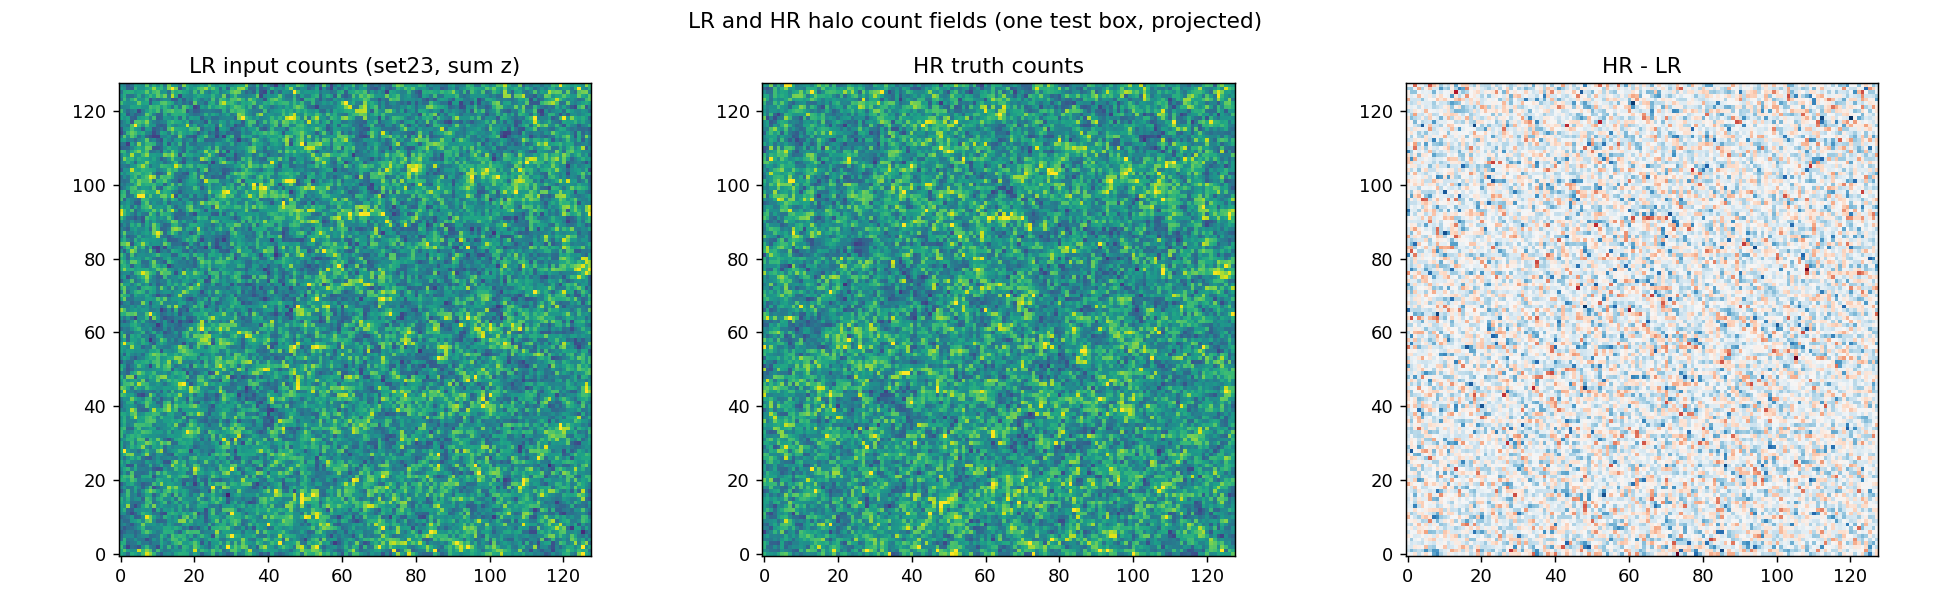
\includegraphics[width=0.9\linewidth]{figures_cmass/data_pair.png}
\caption{One LR/HR pair (projected count map). LR (FastPM, input) and HR
(Quijote N-body, target) share initial conditions and so share large-scale
structure, but differ cell-by-cell.}
\label{fig:srs-datapair}
\end{figure}

\paragraph{Model space (count transform).} The network does not learn on raw
counts; it learns in a compressed ``model space''. The default transform is
$\log(1+n)$, which tames the sparse heavy tail:
\begin{equation}
  y = \log(1+n), \qquad n = \exp(y)-1 \ \ (\text{clamped to } n\ge 0).
  \label{eq:srs-transform}
\end{equation}
Two alternative transforms exist in the code (\texttt{scale}: $n/\text{scale}$;
\texttt{delta}: model space is the overdensity itself), but all reported runs use
$\log(1+n)$. Power spectra are \emph{never} computed in model space; they are
always computed on the physical-count overdensity \SG{Is it okay if this is -1 when there are 0 halos?}
\begin{equation}
  \delta = \frac{n}{\bar n} - 1,
  \label{eq:srs-delta}
\end{equation}
with $\bar n$ the per-box mean count (the \texttt{perbox} setting used in all
runs).

\subsection{Data Pipeline (patching)}
\textit{Located in: \texttt{data/patch\_dataset\_cmass.py},
\texttt{data/patch\_dataset\_real.py} (shared patch ops).}

A model never sees the whole $128^3$ box at once. We cut the box into a
$2\times2\times2$ grid of $64^3$ \textbf{cores} (Table~\ref{tab:srs-notation}).
The cores tile the box exactly (stride $64$), so they reconstruct the box
bit-for-bit with no gaps and no double counting, the dataset's self-test
asserts this. Each model \emph{input} is a core grown by \texttt{pad} voxels on
every side, taken from the true neighbour cells with periodic wrap at the box
edge (\texttt{extract\_patch} uses \texttt{numpy.take(\dots, mode="wrap")}). So
with \texttt{pad}${=}8$ the input is $80^3$ and neighbouring patches overlap by
$2\cdot\texttt{pad}=16$ voxels; the HR \emph{target} is always the bare $64^3$
core. Because each simulation is one continuous periodic box that we crop
ourselves, the patches are real neighbours by construction, there is no data
seam (unlike the Lagrangian patches of \S5). \SG{Isn't the patch construction same in both?}

\begin{table}[t]
\centering
\caption{Notation for the CMASS count-field pipeline.}
\label{tab:srs-notation}
\begin{tabular}{llp{7.2cm}}
\toprule
Symbol & Value & Meaning \\
\midrule
$N_\text{full}$    & $128$ & full box side (voxels) \\
$P$ (\texttt{PATCH}) & $64$ & core side (voxels) \\
$N_\text{patches}$ & $8$ & cores per box ($2{\times}2{\times}2$) \\
\texttt{pad}       & $0$ (Arm A) / $8$ (Arm B) & halo width added to each face by periodic wrap \\
$L_\text{box}$     & $1000\ \mathrm{Mpc}/h$ & box side \\
$\mathbf s$        & $\in\mathbb R^5$ & cosmology vector $(\Omega_m,\Omega_b,h,n_s,\sigma_8)$ \\
$\bar n$           & per-box mean & mean count used to form $\delta=n/\bar n-1$ \\
\bottomrule
\end{tabular}
\end{table}

\begin{figure}[t]
\centering
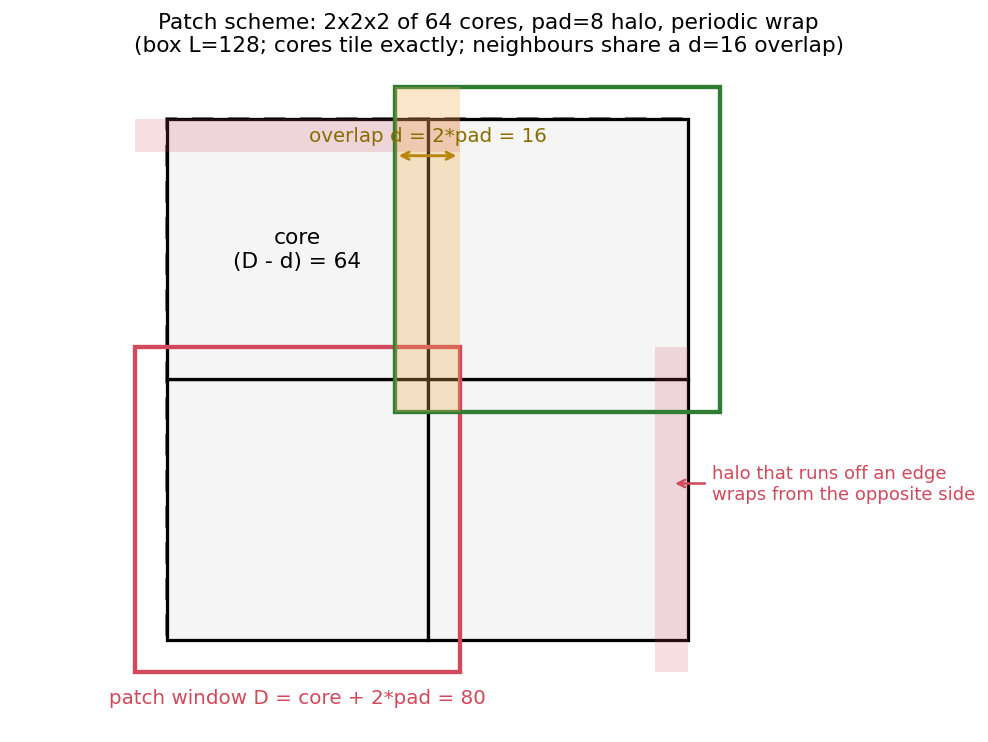
\includegraphics[width=0.82\linewidth]{figures_cmass/pipeline_patching.png}
\caption{Patch scheme. The box is cut into a $2{\times}2{\times}2$ grid of
$64^3$ cores that tile it exactly. With \texttt{pad}${>}0$ each patch is grown by
a halo of real neighbour cells (periodic wrap); only the central core is kept
and placed back.}
\label{fig:srs-patching}
\end{figure}

\paragraph{Per-simulation item.} Indexed by simulation, the dataset returns, for
all $8$ cores at once: the LR patches \texttt{lr\_in} of shape
$(8,\,1,\,64{+}2\,\texttt{pad},\,\cdot,\,\cdot)$ in model space, the HR cores
\texttt{hr\_tgt} of shape $(8,\,1,\,64,\,64,\,64)$, the style $\mathbf s$, and
the simulation index. The trainer flattens the $8$-core axis into the batch.

\begin{algorithm}[H]
\caption{\textsc{ExtractPatches} (one simulation)}
\label{alg:srs-extract}
\begin{algorithmic}[1]
\Require LR box $\mathbf L\in\mathbb R^{1\times128^3}$, HR box $\mathbf H$, \texttt{pad}
\State map $\mathbf L,\mathbf H$ to model space via Eq.~\ref{eq:srs-transform}
\For{$p=0,\dots,7$}
  \State $(i,j,k)\gets\textsc{unravel}(p,(2,2,2))$ \Comment{core origin $(64i,64j,64k)$}
  \State $\mathbf L_p\gets$ core $p$ grown by \texttt{pad} on each face, periodic wrap \Comment{$(64{+}2\,\texttt{pad})^3$}
  \State $\mathbf H_p\gets$ bare core $p$ \Comment{$64^3$}
\EndFor
\State \Return $\{(\mathbf L_p,\mathbf H_p)\}_{p=0}^{7}$, style $\mathbf s$
\end{algorithmic}
\end{algorithm}

\subsection{Model: Input/Output Specification}
\textit{Implementation: \texttt{map2map/models/styled\_srsgan.py}
(\texttt{G\_correct}, \texttt{D\_const}).}

\paragraph{What the generator computes.} The generator is a
\textbf{same-resolution residual} network: it does not change the grid size, and
it predicts a correction that is \emph{added} to the input. In model space,
\begin{equation}
  \mathrm{SR} \;=\; \mathrm{LR} \;+\; G(\mathrm{LR},\,\mathbf s,\,\mathbf z),
  \label{eq:srs-residual}
\end{equation}
where $\mathbf s$ is the cosmology vector and $\mathbf z$ is an injected noise
field (see below). Inputs and outputs are listed in
Table~\ref{tab:srs-model-io}; the generator is run once per core (the $8$ cores
of a box form a batch).

\begin{table}[t]
\centering
\caption{Tensors consumed/produced by the generator \texttt{G\_correct} for one
core (batch dimension omitted). Here $D=64{+}2\,\texttt{pad}$.}
\label{tab:srs-model-io}
\begin{tabular}{lll}
\toprule
Symbol & Shape & Meaning \\
\midrule
$\mathbf x$ (\texttt{x})       & $(1,D,D,D)$ & LR patch, model space (input) \\
$\mathbf s$ (\texttt{style})   & $(5,)$      & cosmology vector \\
$\mathbf z$ (\texttt{noise\_list}) & $2\cdot\texttt{num\_blocks}$ cubes $(1,D,D,D)$ & injected noise; fixed at inference, random in training \\
$G(\cdot)$                     & $(1,D,D,D)$ & predicted residual $\delta$ (added to $\mathbf x$) \\
\bottomrule
\end{tabular}
\end{table}

\paragraph{Internal composition.} $G$ is a constant-resolution StyleGAN2-style
network (no up/down-sampling), built from:
\begin{enumerate}
  \item \texttt{block0}: a $1{\times}1{\times}1$ style-modulated convolution
  (\texttt{ConvStyled3d}) lifting the $1$-channel input to $c_0$ channels,
  followed by a leaky ReLU.
  \item \texttt{num\_blocks} ($=4$) constant-resolution H-blocks
  (\texttt{HBlock\_const}). Each block, in order: inject noise $\to$
  $3{\times}3{\times}3$ \texttt{ConvStyled3d} (periodic ``circular'' padding)
  $\to$ leaky ReLU $\to$ inject noise $\to$ $3{\times}3{\times}3$
  \texttt{ConvStyled3d} $\to$ leaky ReLU $\to$ a $1{\times}1{\times}1$ projection
  to the output channel, accumulated into a running output $y$. The final return
  is $\mathbf x + y$ (Eq.~\ref{eq:srs-residual}).
\end{enumerate}
The channel widths come from \texttt{chan\_base} ($=128$) halved per block and
clamped to $[64,512]$. Two mechanisms make the convolutions depend on side
information:
\begin{itemize}
  \item \textbf{Style modulation.} \texttt{ConvStyled3d} is the StyleGAN2
  modulated/demodulated convolution: the cosmology vector $\mathbf s$ scales the
  convolution weights, so the same network behaves differently for different
  cosmologies. This is the only path by which $\mathbf s$ enters.
  \item \textbf{Noise injection.} Each \texttt{ConvStyled3d} is preceded by a
  per-channel learned-standard-deviation noise add (\texttt{\_NoiseInject}). At
  training time the noise is fresh Gaussian each call; at inference a
  \emph{fixed} list of noise cubes (seeded, built by \texttt{build\_noise\_list})
  is reused so outputs are reproducible. The noise is what lets the model produce
  a plausible small-scale field rather than a single blurred guess.
\end{itemize}

\paragraph{Discriminator.} \texttt{D\_const} is a constant-input-resolution
critic conditioned on the same style $\mathbf s$. It runs a head
\texttt{ConvStyled3d} then \texttt{num\_blocks} strided down-blocks (each a
periodic $3{\times}3{\times}3$ \texttt{ConvStyled3d} $+$ leaky ReLU $+$
$2{\times}$ average pool), a $1{\times}1{\times}1$ tail, and a final
$1{\times}1{\times}1$ projection to one channel, averaged over space to a single
logit per core.

\subsection{Training Step}
\textit{Located in: \texttt{train\_patch\_cmass.py}.}

The generator is trained per core (stitching is \emph{not} part of the
gradient). The total generator loss is a weighted sum of three terms,
\begin{equation}
  \mathcal L_G \;=\; \lambda_\text{adv}\,\mathcal L_\text{adv}
                  + \lambda_\text{rec}\,\mathcal L_\text{rec}
                  + \lambda_\text{pk}\,\mathcal L_\text{pk},
  \label{eq:srs-lossG}
\end{equation}
with (defaults from the original run script; see the protocol update below for
the values now in use):
\begin{itemize}
  \item \textbf{Reconstruction} $\mathcal L_\text{rec}=\lVert \mathrm{SR}-\mathrm{HR}\rVert_1$,
  a plain $L_1$ in model space (optionally Gaussian-smoothed; smoothing off in
  all runs).
  \item \textbf{Power-spectrum} $\mathcal L_\text{pk}$, the mean-squared error
  between the $\log_{10}$ power spectra of SR and HR, computed on the
  \emph{physical-count overdensity} of the $64^3$ core (Eqs.~\ref{eq:srs-transform}--\ref{eq:srs-delta}),
  Hann-windowed, with the HR side detached:
  \begin{equation}
    \mathcal L_\text{pk} = \frac{1}{|K|}\sum_{k\in K}
      \big(\log_{10} P_\text{SR}(k) - \log_{10} P_\text{HR}(k)\big)^2 .
    \label{eq:srs-pkloss}
  \end{equation}
  \item \textbf{Adversarial} $\mathcal L_\text{adv}=\mathrm{softplus}\!\big({-}D(\mathrm{SR},\mathbf s)\big)$,
  the non-saturating GAN generator loss.
\end{itemize}

\paragraph{Protocol update: what region the reconstruction and adversarial
terms see.} A \texttt{--pad-loss} setting controls how much of the generator's
output the $L_1$ and adversarial terms are computed on, independent of
\texttt{pad} itself:
\begin{itemize}
  \item \texttt{crop} (trim-aware, the setting used for Arm B above): the loss
  is computed only on \textsc{cropInterior}$(G(\mathbf x,\mathbf s),\,\texttt{pad})$,
  the $64^3$ core that is actually kept at inference time, against the bare
  $64^3$ HR core. The model is trained on exactly the region it will be graded
  on.
  \item \texttt{full}: the loss is computed on the whole $(64{+}2\,\texttt{pad})^3$
  output, against a correspondingly padded HR target (the dataset's
  \texttt{pad\_target} option). The model is trained as if the halo region it
  will later be trimmed off also mattered.
\end{itemize}
Concretely, let $\texttt{loss\_crop}=\texttt{pad}$ under \texttt{crop} and $0$
under \texttt{full}; every place above that writes $\mathrm{SR}$ means
$\textsc{cropInterior}(G(\mathbf x,\mathbf s),\,\texttt{loss\_crop})$, and the
Hann window and $P(k)$ estimator in $\mathcal L_\text{pk}$ are sized to match.
This is a controlled test of two ways padding could fail to help: see the
protocol-update subsection below for the result.

The discriminator is trained with the non-saturating GAN loss plus a lazy $R_1$
gradient penalty applied every \texttt{r1\_every} steps:
\begin{equation}
  \mathcal L_D = \mathrm{softplus}\!\big({-}D(\mathrm{HR})\big)
               + \mathrm{softplus}\!\big(D(\mathrm{SR})\big)
               + \tfrac{1}{2}\lambda_{R_1}\,\mathbb E\big\lVert \nabla_{\!x} D(x,\mathbf s)\big\rVert^2 .
  \label{eq:srs-lossD}
\end{equation}

\begin{algorithm}[H]
\caption{CMASS patch-GAN training step (one batch of cores)}
\label{alg:srs-train}
\begin{algorithmic}[1]
\Require LR patches $\mathbf x$, HR targets $\mathbf h$ (padded iff \texttt{pad-loss=full}),
         style $\mathbf s$, \texttt{pad}, \texttt{loss\_crop} ($=\texttt{pad}$ if \texttt{crop} else $0$),
         weights $\lambda_\text{adv},\lambda_\text{rec},\lambda_\text{pk},\lambda_{R_1}$
\Statex \textbf{// Discriminator}
\State $\hat{\mathbf h}\gets \textsc{cropInterior}\big(G(\mathbf x,\mathbf s),\,\texttt{loss\_crop}\big)$ \Comment{no grad}
\State $\mathcal L_D \gets \mathrm{softplus}({-}D(\mathbf h,\mathbf s)) + \mathrm{softplus}(D(\hat{\mathbf h},\mathbf s))$
\If{step $\bmod\ \texttt{r1\_every} = 0$} $\mathcal L_D \mathrel{+}= \tfrac12\lambda_{R_1}\texttt{r1\_every}\cdot R_1(D,\mathbf h,\mathbf s)$ \EndIf
\State update $D$ (Adam, grad-clip)
\Statex \textbf{// Generator}
\State $\hat{\mathbf h}\gets \textsc{cropInterior}\big(G(\mathbf x,\mathbf s),\,\texttt{loss\_crop}\big)$
\State $\mathcal L_\text{adv}\gets \mathrm{softplus}({-}D(\hat{\mathbf h},\mathbf s))$
\State $\mathcal L_\text{rec}\gets \lVert \hat{\mathbf h}-\mathbf h\rVert_1$
\State $\mathcal L_\text{pk}\gets$ Eq.~\ref{eq:srs-pkloss} on Hann-windowed overdensity of $\hat{\mathbf h}$, $\mathbf h$
       (skip if $\lambda_\text{pk}{=}0$)
\State $\mathcal L_G \gets \lambda_\text{adv}\mathcal L_\text{adv}+\lambda_\text{rec}\mathcal L_\text{rec}+\lambda_\text{pk}\mathcal L_\text{pk}$
\State update $G$ (Adam, grad-clip)
\end{algorithmic}
\end{algorithm}

\paragraph{Validation and checkpoint selection.} After each epoch we stitch the
full $128^3$ SR box for up to $40$ validation sims and report the stitched
$L_1$/voxel and the stitched-$128$ power-spectrum RMS against HR
(\S\ref{sec:srs-eval}, Eq.~\ref{eq:srs-pkrms}). A \texttt{--select} setting
chooses which of the two the saved \texttt{best.pt} tracks: \texttt{pk} (the
original setting, lowest stitched validation Pk RMS) or \texttt{l1} (lowest
stitched validation $L_1$/voxel). Selection is always on the stitched full box,
not the per-core training loss. Runs that also train with $\lambda_\text{pk}{=}0$
use \texttt{--select l1}, since selecting on Pk RMS while not training on it
would reintroduce the same metric leak in a different place.

\subsection{Inference}
\textit{Located in: \texttt{infer\_stitch\_cmass.py}.}

For one simulation: load the LR $128^3$ count box, map it to model space, run $G$
on each of the $8$ cores (with the periodic-wrap halo in Arm B), crop the halo,
stitch the cores into a $128^3$ model-space box, invert the transform to physical
counts, and clamp. \SG{are all outputs later mapped to integers, or are we fine with non-integer number of halos?} The injected noise list is fixed (seeded) so the output is
reproducible.

\begin{algorithm}[H]
\caption{CMASS inference + stitch (one simulation)}
\label{alg:srs-infer}
\begin{algorithmic}[1]
\Require LR box $\mathbf L$, style $\mathbf s$, trained $G$, mode (naive/overlap), fixed noise $\mathbf z$
\State $\texttt{pad}\gets 0$ if naive else value from checkpoint ($8$)
\State map $\mathbf L$ to model space (Eq.~\ref{eq:srs-transform})
\For{$p=0,\dots,7$}
  \State $\mathbf x_p\gets$ patch $p$ (core grown by \texttt{pad}, periodic wrap)
  \State $\mathbf c_p\gets \textsc{cropInterior}\big(G(\mathbf x_p,\mathbf s,\mathbf z),\,\texttt{pad}\big)$ \Comment{$64^3$ core, model space}
\EndFor
\State $\mathbf S\gets \textsc{stitch}(\{\mathbf c_p\})$ \Comment{$128^3$, model space}
\State $\mathbf S\gets \exp(\mathbf S)-1$, clamp to $[0,\,C_\text{max}{=}200]$, replace NaN/Inf \Comment{physical counts}
\State \Return $\mathbf S$
\end{algorithmic}
\end{algorithm}

\subsection{Crop Stitching}

Stitching is \textbf{direct placement with no averaging}. Adjacent cores tile the
box exactly (stride $64$, no overlap between cores once the halo is dropped), so
each core's $64^3$ output is written straight into its slot. In Arm B the $80^3$
patch is corrected and only its central $64^3$ core is kept; the overlap halo is
context for the convolution, never written to the output.

\begin{algorithm}[H]
\caption{\textsc{Stitch} ($8$ cores $\to$ $128^3$)}
\label{alg:srs-stitch}
\begin{algorithmic}[1]
\Require cores $\{\mathbf c_p\}_{p=0}^{7}$, each $1\times64^3$
\State $\mathbf S\gets \mathbf 0\in\mathbb R^{1\times128^3}$
\For{$p=0,\dots,7$}
  \State $(i,j,k)\gets\textsc{unravel}(p,(2,2,2))$
  \State $\mathbf S[:,\,64i{:}64i{+}64,\,64j{:}\cdots,\,64k{:}\cdots]\gets \mathbf c_p$ \Comment{direct assignment}
\EndFor
\State \Return $\mathbf S$
\end{algorithmic}
\end{algorithm}

\subsection{Evaluation}
\label{sec:srs-eval}
\textit{Located in: \texttt{analysis/eval\_seam\_cmass.py},
\texttt{analysis/diag\_cmass.py}, \texttt{analysis/match\_stats\_cmass.py},
\texttt{analysis/power\_spectrum.py}, \texttt{inference/nde.py},
\texttt{evaluate.py}.}

We evaluate the SR field against HR at three levels: a seam check (does stitching
leave a join?), field statistics (does SR have the right structure?), and
cosmology (does SR give the same parameter posterior as HR?).

\paragraph{Power-spectrum summaries.} On the count overdensity (Eq.~\ref{eq:srs-delta})
we report the power spectrum $P(k)$, the transfer ratio, and the cross-coherence:
\begin{equation}
  T(k) = \frac{P_\text{SR}(k)}{P_\text{HR}(k)},
  \qquad
  r(k) = \frac{P_{\text{SR},\text{HR}}(k)}{\sqrt{P_\text{SR}(k)\,P_\text{HR}(k)}} .
  \label{eq:srs-Tr}
\end{equation}
$T(k)=1$ means SR has the right \emph{amount} of power at scale $k$ (amplitude);
$r(k)=1$ means SR has the structure in the right \emph{place} (phase). The
scalar power-spectrum error used for checkpoint selection and seam reporting is
the log-RMS over the resolved $k$-bins:
\begin{equation}
  \mathrm{PkRMS}_{\log_{10}} = \sqrt{\frac{1}{|K|}\sum_{k\in K}
    \big(\log_{10} P_\text{SR}(k) - \log_{10} P_\text{HR}(k)\big)^2 } .
  \label{eq:srs-pkrms}
\end{equation}

\paragraph{Seam diagnostic.} \texttt{eval\_seam\_cmass.py} bins the per-cell
count error $|{\mathrm{SR}-\mathrm{HR}}|$ by distance to the nearest core face
and forms a per-position error profile along each axis. The headline number is
the \textbf{$x{=}64$ internal-seam excess}: the error on the internal core
boundary plane divided by the interior error. A value near $1$ means stitching
leaves no seam. The box edge $x{=}0$ is a periodic-boundary control.

\paragraph{Field-match statistics.} \texttt{match\_stats\_cmass.py} reports, over
$16$ test boxes: the total-count ratio $\sum\mathrm{SR}/\sum\mathrm{HR}$, the
void fraction (cells $<0.5$), the real-space cell standard-deviation ratio
$\mathrm{std}(\mathrm{SR})/\mathrm{std}(\mathrm{HR})$ (a blur check), and the
cross-coherence $r(k)$ at large ($k<0.05$) and small ($k>0.2$) scales.

\paragraph{Cosmology (posterior consistency).} This is the strongest ``does SR
match HR'' test. We voxel-count $\to$ overdensity $\to$ $P(k)$ for every box, then
train a neural density estimator $q(\theta\mid P(k))$ on the training split using
\texttt{sbi} (\texttt{SNPE\_C} with a neural-spline-flow density estimator,
\texttt{inference/nde.py}); the summary is $\log_{10}P(k)$. We train one estimator
on HR ($q_\text{HR}$) and one on each SR arm ($q_\text{SR}$). For each test box we
draw $2000$ posterior samples from each, fit a Gaussian per parameter, and report
the per-parameter Gaussian KL (\texttt{evaluate.py}):
\begin{equation}
  \mathrm{KL}\big(\mathcal N(\mu_\text{HR},\sigma_\text{HR})\,\Vert\,\mathcal N(\mu_\text{SR},\sigma_\text{SR})\big)
  = \tfrac12\!\left[\log\frac{\sigma_\text{SR}^2}{\sigma_\text{HR}^2}
    + \frac{\sigma_\text{HR}^2+(\mu_\text{HR}-\mu_\text{SR})^2}{\sigma_\text{SR}^2} - 1\right].
  \label{eq:srs-kl}
\end{equation}
$\mathrm{KL}=0$ means SR gives the identical cosmology posterior to HR. The raw LR
field (no model), pushed through the same pipeline, is the control SR must beat.

We report this comparison in two forms, and it matters which is which:
\begin{itemize}
  \item \textbf{Cross-fidelity (primary).} $q_\text{SR}$ is trained on SR power
  spectra but \emph{evaluated on the HR} $P(k)$ of each test simulation, and
  compared to $q_\text{HR}$ evaluated on the same HR $P(k)$. This is the
  deployment scenario the project targets: HR simulations are too expensive to
  train an inference model on, so the inference model is trained on cheap SR
  output and must still work when applied to (HR-like) reality. The comparison
  against an LR-trained estimator on the same HR data measures whether sampling
  in HR space (SR) survives the distribution shift better than staying in LR
  space. This metric never appears in the training loss.
  \item \textbf{Own-data (secondary).} $q_\text{SR}$ trained and evaluated on SR
  vs $q_\text{HR}$ trained and evaluated on HR, each pipeline end-to-end on
  its own field type.
\end{itemize}

\subsection{Best-Run Configuration}
\textit{Run script: \texttt{scripts/train\_patch\_cmass.slurm}; checkpoints
\texttt{checkpoints/patch\_cmass\_\{A,B\}/best.pt}.}

Both arms use the identical configuration below; they differ only in \texttt{pad}
($0$ for Arm~A, $8$ for Arm~B). This is the configuration behind every number
in \S\ref{sec:srs-results}--\S\ref{sec:srs-next}.

\begin{lstlisting}[language=bash]
--transform log1p   --nbar perbox        # log(1+n) model space; per-box nbar
--epochs 30         --sims-per-batch 1    # patch-batch = 8 cores per step
--chan-base-g 128   --chan-base-d 64  --num-blocks 4
--lambda-adv 1.0    --lambda-rec 2.0  --lambda-pk 2.0   # generator weights
--lambda-r1 10.0    --r1-every 16                       # lazy R1
--lr-g 1e-4 --lr-d 1e-4  --beta1 0.0 --beta2 0.99       # Adam
--grad-clip 1.0     --val-max-sims 40    --select pk    # select on Pk RMS
\end{lstlisting}

The best checkpoint per arm is the one with the lowest stitched validation Pk RMS
(Eq.~\ref{eq:srs-pkrms}):

\begin{center}
\begin{tabular}{lc}
\toprule
arm & best stitched val PkRMS$_{\log_{10}}$ \\
\midrule
Arm A, naive (pad $0$)  & $0.0947$ \\
Arm B, overlap (pad $8$) & $0.0963$ \\
\bottomrule
\end{tabular}
\end{center}

\paragraph{Protocol update.} Following the mentor meeting reported in
\S\ref{sec:srs-followup}, the configuration above is no longer the one we train
with. Three settings changed:
\begin{lstlisting}[language=bash]
--lambda-pk 0.0      # power-spectrum term OFF (it was also our main metric)
--pad-loss crop|full # trim-aware vs trim-unaware padding, see below
--select l1          # select on stitched L1, not the term we removed
\end{lstlisting}
All results in \S\ref{sec:srs-followup} use this configuration. Runs under the
original configuration above (Arm A, Arm B, and everything derived from them in
\S\ref{sec:srs-results}--\S\ref{sec:srs-next}) remain valid as a record of that
protocol; they are superseded, not invalidated, by the update.

\subsection{Results: Does SR Match HR?}
\label{sec:srs-results}

All numbers are on the $200$-box test split unless noted.

\paragraph{1. Power spectrum (statistics).} Across the test set the SR power
spectrum tracks HR at every scale, and Arm A beats the no-model LR control on the
overall log-RMS (Fig.~\ref{fig:srs-srvshr}, computed by
\texttt{analysis/plot\_sr\_vs\_hr.py}).

\begin{table}[h]
\centering
\caption{SR vs HR power-spectrum agreement, $200$ test boxes. Transfer
$T(k)=P_X/P_\text{HR}$ (Eq.~\ref{eq:srs-Tr}); $1.0$ is perfect.}
\label{tab:srs-pk}
\begin{tabular}{lccc}
\toprule
field (vs HR) & PkRMS$_{\log_{10}}$ & $T$ at large scales ($k{<}0.1$) & $T$ at small scales ($k{>}0.3$) \\
\midrule
SR (Arm A, naive)    & $\mathbf{0.0607}$ & $0.95$ & $1.04$ \\
SR (Arm B, overlap)  & $0.0645$ & $0.93$ & $0.88$ \\
LR (no model, control) & $0.0641$ & $1.01$ & $1.01$ \\
\bottomrule
\end{tabular}
\end{table}

\begin{figure}[t]
\centering
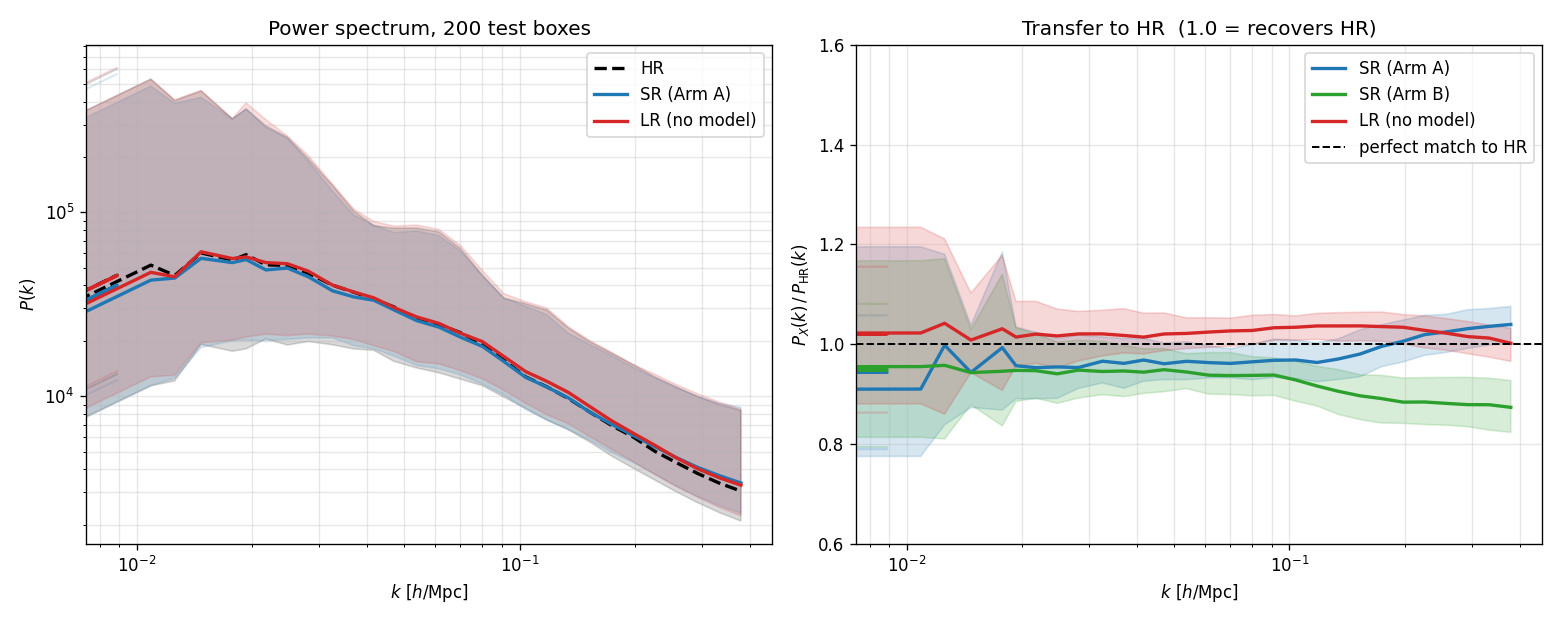
\includegraphics[width=0.98\linewidth]{figures_cmass/sr_vs_hr_pk.png}
\caption{\textbf{Left:} $P(k)$ of HR, SR (Arm A), and LR over $200$ test boxes
(median $+$ $16/84\%$ band). \textbf{Right:} transfer to HR; $1.0$ recovers HR.
SR (Arm A) sits near $1$ at all scales; Arm B's overlap blending slightly
suppresses small-scale power (transfer $0.88$).}
\label{fig:srs-srvshr}
\end{figure}

\paragraph{2. Field structure.} Beyond the power spectrum, SR keeps the field
structure of HR (Arm A, $16$ test boxes, \texttt{match\_stats\_cmassA.txt}):

\begin{table}[h]
\centering
\caption{SR vs HR field-match statistics (Arm A).}
\label{tab:srs-match}
\begin{tabular}{lll}
\toprule
quantity & value & reading \\
\midrule
total count ratio $\sum\mathrm{SR}/\sum\mathrm{HR}$ & $0.965\pm0.172$ & counts conserved on average; large per-box scatter \\
real-space std ratio & $1.008\pm0.100$ & clustering amplitude matches; not blurred \\
void fraction SR / HR ($<0.5$) & $0.855$ / $0.833$ & SR keeps voids empty, like HR \\
cross-coherence $r$, $k<0.05$ & $0.951$ & large-scale structure matches cell-by-cell \\
cross-coherence $r$, $k>0.2$ & $0.403$ & small-scale structure decorrelates \\
\bottomrule
\end{tabular}
\end{table}

\paragraph{3. Cosmology.} The cosmology comparison in the original report used
mislabeled cosmologies, an indexing bug we describe and fix in
\S\ref{sec:srs-correction}, so those numbers are not shown here. With correct
labels a single box constrains $\Omega_m$ and $\sigma_8$; at the power spectrum
level the raw LR field is already HR-like, while at the field level an SR-trained
posterior transfers to HR and an LR-trained one does not
(\S\ref{sec:srs-correction}, Table~\ref{tab:srs-corrected}).

\paragraph{4. Seam.} Neither arm introduces a stitching seam: the $x{=}64$
internal-seam excess is $\approx1$ for both
(Table~\ref{tab:srs-seam}, Fig.~\ref{fig:srs-seam}). Arm A shows a mild generic
ripple near \emph{any} boundary plane (seam-distance ratio $1.17$); Arm B's
overlap removes it ($1.00$) at a small cost in Pk RMS.

\begin{table}[h]
\centering
\caption{Seam and stitched-fidelity metrics, $200$ test boxes. ``Excess'' is
boundary error over interior error; $\approx1$ means no seam.}
\label{tab:srs-seam}
\begin{tabular}{lccp{5.2cm}}
\toprule
metric & Arm A naive & Arm B overlap & reading \\
\midrule
$x{=}64$ internal-seam excess & $0.9934$ & $0.9998$ & no internal seam either arm \\
seam-distance ratio ($d{=}0/d{\ge}8$) & $1.1729$ & $1.0032$ & generic boundary ripple, removed by overlap \\
$x{=}0$ periodic edge (control) & $0.9930$ & $0.9993$ & box edge behaves like interior \\
stitched PkRMS$_{\log_{10}}$ vs HR & $0.0637$ & $0.0678$ & stitched power-spectrum match \\
\bottomrule
\end{tabular}
\end{table}

\begin{figure}[t]
\centering
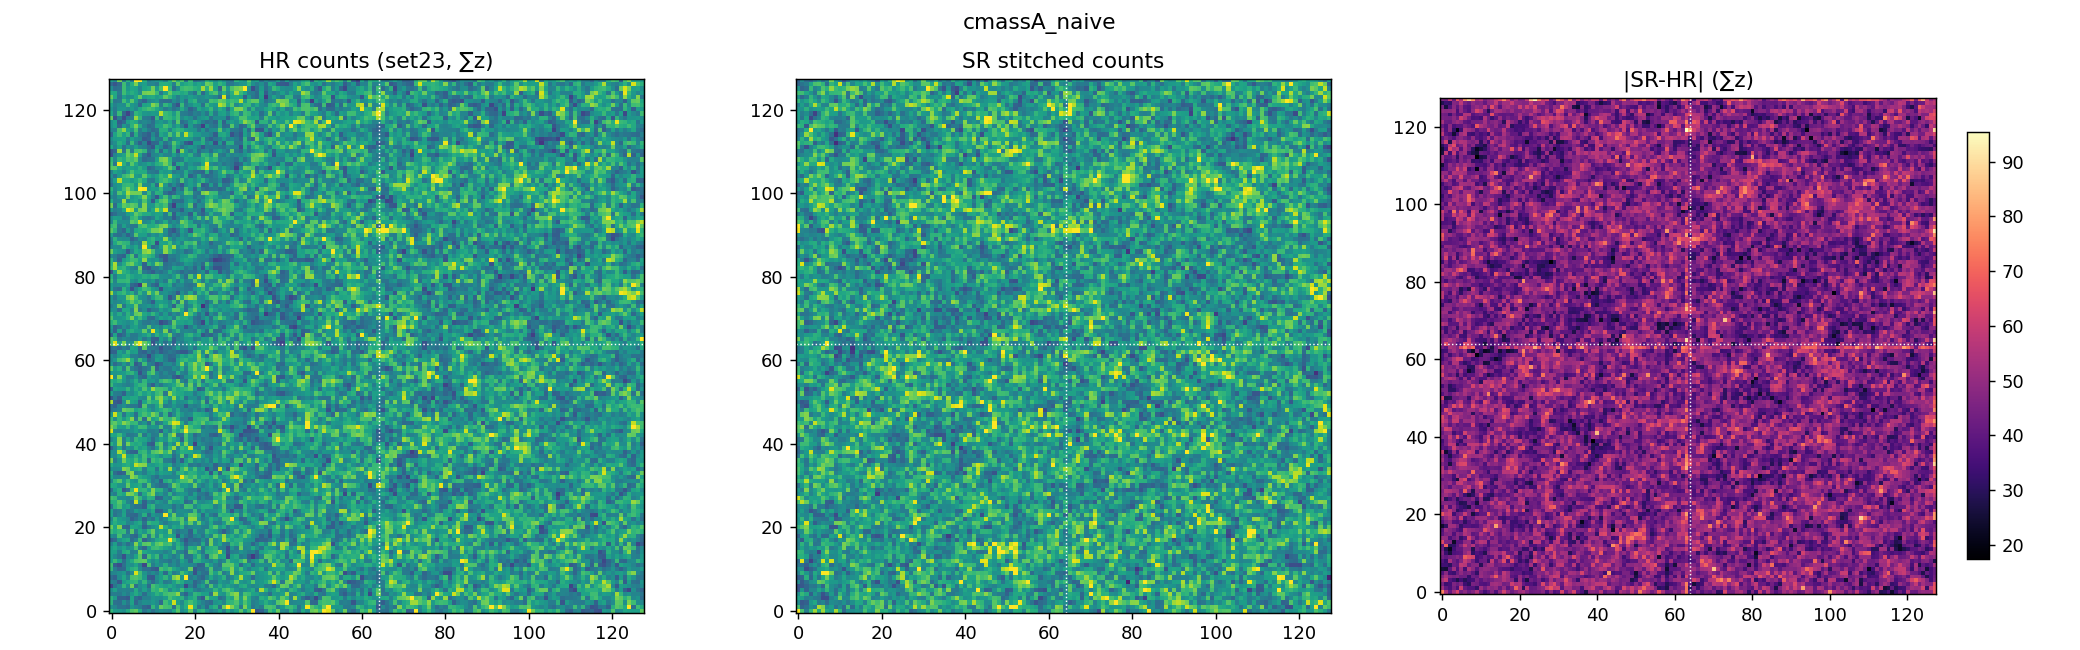
\includegraphics[width=0.95\linewidth]{figures_cmass/seam_cmassA_naive_slice.png}
\caption{Projected count maps for one test box (Arm A): HR, stitched SR, and the
absolute residual $|\mathrm{SR}-\mathrm{HR}|$. White dotted lines mark the
$x{=}64$, $y{=}64$ core boundaries; the residual shows no elevated ridge along
them.}
\label{fig:srs-seam}
\end{figure}

\paragraph{Per-scale diagnostic panels.} Figure~\ref{fig:srs-pkpanel} shows the
full-box $P(k)$, transfer, and cross-coherence for Arm A. The transfer sits near
$1$ at all scales (right amount of power); the cross-coherence is near $1$ at
large scales and falls toward small scales (structure placement is recovered at
large scales only). The per-patch panel
(\texttt{figures\_cmass/pk\_panel\_patch\_cmassAfix.png}) and the projection panels
(\texttt{projection\_box\_cmassAfix\_set23.png},
\texttt{projection\_patch\_cmassAfix\_set23\_p0.png}) tell the same story; Arm~B's
panels carry the \texttt{cmassB} suffix.

\begin{figure}[t]
\centering
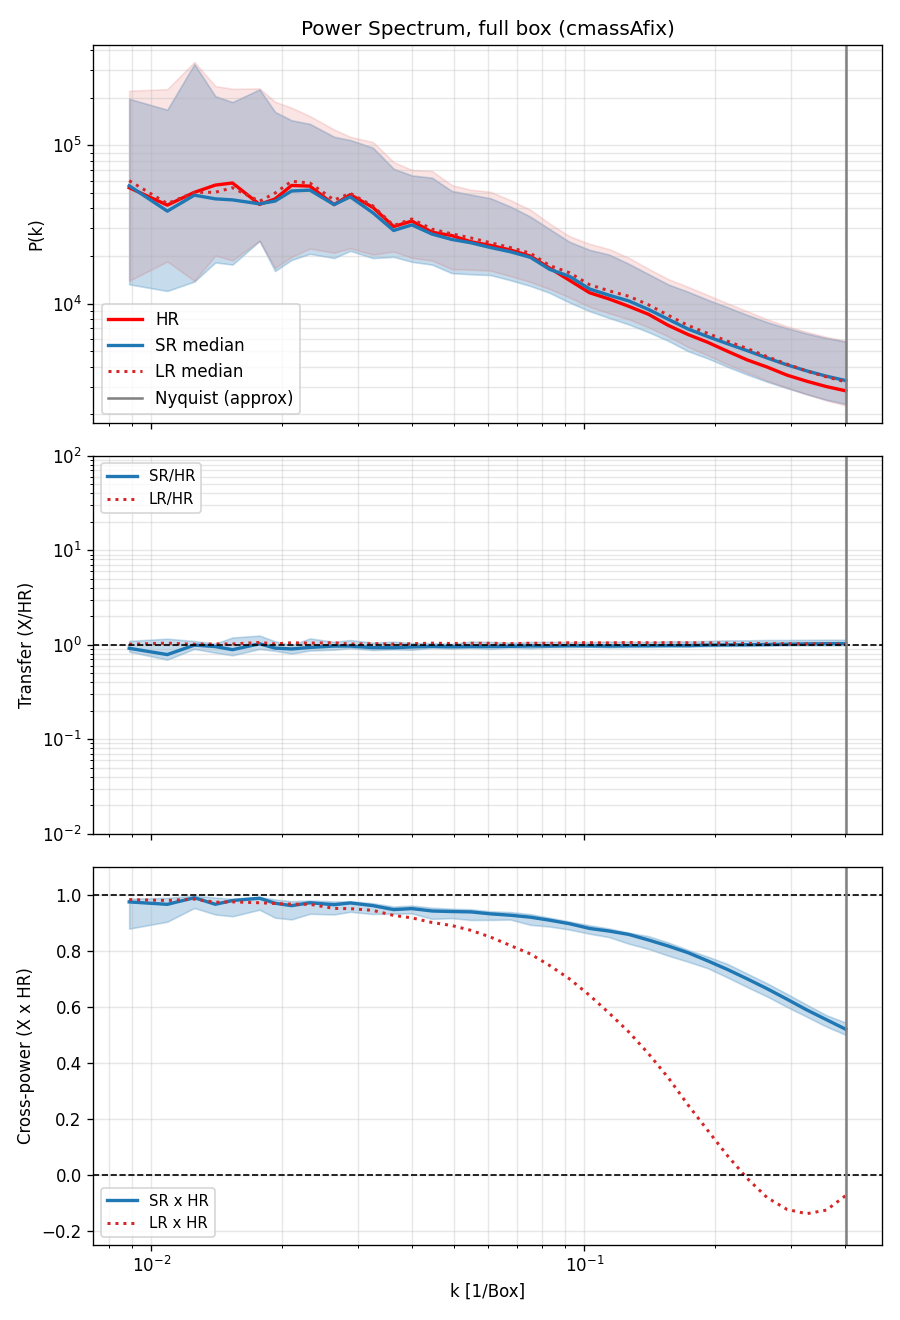
\includegraphics[width=0.5\linewidth]{figures_cmass/pk_panel_box_cmassAfix.png}
\caption{Full-box diagnostic for the conditioned generator (fiducial cosmology,
$16$ test boxes): $P(k)$ of HR (red), SR (blue median $+$ band), and LR (dotted
red); transfer $T(k)=P_X/P_\text{HR}$ on a linear axis with the 16 to 84
percentile band for both SR and LR, the legend reporting the RMS deviation of
each ratio from unity; and cross-coherence $r(k)$. The SR median transfer sits
below unity for $k<0.1$, a systematic large-scale power deficit of roughly 5 to
10 percent, while LR sits slightly above unity; SR does not tighten the transfer
scatter relative to LR. In $r(k)$, SR stays near unity to smaller scales while
LR decorrelates.}
\label{fig:srs-pkpanel}
\end{figure}

\subsection{Diagnostic: What is NOT Working}

\paragraph{Small-scale structure decorrelates, and this is fundamental.} SR
matches HR cell-by-cell at large scales ($r{=}0.95$ for $k<0.05$) but loses the
match at small scales ($r{=}0.40$ for $k>0.2$, Table~\ref{tab:srs-match}). This
is not a capacity bug: it is set by how much information the LR input carries
about HR. LR and HR share large-scale modes but the voxel-by-voxel LR$\leftrightarrow$HR
correlation is only $\approx0.06$, so the exact small-scale realization is simply
not present in the input. The model can match the small-scale \emph{statistics}
(transfer $\approx1$, real-space std ratio $1.008$) but cannot reproduce the
exact placement of individual halos. The noise injection
(Eq.~\ref{eq:srs-residual}) exists precisely because of this: it draws a
plausible small-scale field rather than regressing to a blur.

\paragraph{Per-box total-count scatter.} The total halo count is conserved on
average but with $\sim17\%$ per-box scatter ($\sum\mathrm{SR}/\sum\mathrm{HR}=
0.965\pm0.172$). A count-aware output head (predict a rate and sample Poisson
counts) would tighten this; it is the one clearly addressable imperfection. \SG{I would think this isn't necessary to fix, we don't care about the number of halos after all.}

\paragraph{Overlap suppresses small-scale power.} Arm B's overlap blending lowers
the small-scale transfer to $0.88$ (Table~\ref{tab:srs-pk}), so on the power
spectrum the naive Arm A is the better super-resolver. Overlap removes a small
generic boundary ripple but buys no fidelity, because on this continuous count
data there is no real seam to fix, the clean version of the mentor 2.1 vs 2.2
comparison.

\paragraph{Where the cosmology value is.} At the power spectrum level the raw LR
field is already close to HR, since they share large-scale modes, so the power
spectrum is a forgiving summary with little headroom. The model's value is at the
field level (variance, voids, small-scale structure), which the power spectrum
summary is insensitive to. The corrected cross-fidelity in
\S\ref{sec:srs-correction} bears this out: SR and LR are indistinguishable at the
power spectrum level, but at the field level an SR-trained posterior transfers to
HR while an LR-trained one does not.

\subsection{What I'm Trying Next}
\label{sec:srs-next}

The diagnostics above point to one limit that may be fundamental (small-scale
decorrelation) and a few that are clearly fixable (count scatter, small-scale
realism). The plan below is ordered so that we \emph{measure} the limit before
spending effort trying to beat it. None of these results are in yet; this is the
roadmap, not an experiment log.

\paragraph{Step 0, measure the information ceiling first.} Before trying to
improve the small-scale match, we need to know whether $r{=}0.40$ at small scales
(Table~\ref{tab:srs-match}) is the best any model could do from this input, or a
weakness of the current one. Two cheap diagnostics settle it:
\begin{itemize}
  \item \textbf{LR$\leftrightarrow$HR cross-coherence $r_\text{LR,HR}(k)$.} The
  cross-coherence of the \emph{raw input} against HR (no model) is the ceiling:
  no function of LR can place small-scale structure better than the input
  already correlates with HR. If $r_\text{SR,HR}(k)\approx r_\text{LR,HR}(k)$ at
  small $k$, the model is already at the ceiling and the limit is fundamental;
  if it sits well below, there is recoverable structure left on the table. (Only
  per-box $P(k)$ is currently saved, not the cross-spectrum, so this needs one
  re-run that keeps the fields.)
  \item \textbf{No-noise ablation.} Train the same generator with the noise
  injection off (a plain regressor). Theory predicts this should \emph{raise} the
  small-scale cross-coherence a little (a regressor targets the conditional mean,
  the best cell-by-cell predictor) but \emph{lower} the small-scale transfer well
  below $1$ (the conditional mean is blurry). Seeing exactly that trade-off would
  confirm that the noise/GAN is the right choice for a power-spectrum target, and
  would quantify how much cell-by-cell accuracy is being traded for correct
  statistics.
\end{itemize}

\paragraph{Step 1, fix the count scatter and small-scale realism (independent
of the ceiling).} These help regardless of what Step 0 finds:
\begin{itemize}
  \item \textbf{Count-aware (Poisson) output head.} Instead of predicting a
  count directly, predict a non-negative rate $\lambda$ per cell and sample the
  count as $n\sim\mathrm{Poisson}(\lambda)$. Halo counts are discrete and sparse,
  so a Poisson head models the small-scale graininess as actual shot noise rather
  than a smeared residual, and should tighten the $\sim17\%$ per-box total-count
  scatter (Table~\ref{tab:srs-match}), the one clearly addressable imperfection.
  \item \textbf{Explicit statistics terms in the loss.} Add a one-point PDF /
  variance matching term so small-scale sharpness is enforced directly, rather
  than relying on the adversarial term alone to find it.
  \item \textbf{Loss rebalance.} The current weights are $\lambda_\text{rec}{=}2$,
  $\lambda_\text{pk}{=}2$, $\lambda_\text{adv}{=}1$
  (Eq.~\ref{eq:srs-lossG}). The $L_1$ term blurs; lowering it and raising the
  adversarial weight should push toward correct statistics, at a known cost in
  cell-by-cell accuracy, per the same trade-off as the no-noise ablation.
\end{itemize}

\paragraph{Step 2, extract more of the available information (only if Step 0
shows headroom).} If $r_\text{SR,HR}$ sits below the LR$\leftrightarrow$HR
ceiling, the model is under-using its input. A larger receptive field, or feeding
each patch more neighbour context, would let it use more of the LR field to
predict the residual. This only helps if there is headroom to recover.

\paragraph{Step 3, raise the ceiling by changing the \emph{input}, not the
model.} The small-scale cell-by-cell limit is set by the information in the LR
input (the voxel-by-voxel LR$\leftrightarrow$HR correlation is only
$\approx0.06$). No amount of model capacity raises that; only more informative
inputs do. Candidates: feed the shared small-scale \emph{initial conditions}
(which the coarse LR count field has discarded), or add the LR velocity / particle
fields. This is the only route to a meaningful gain in small-scale cross-coherence,
and is the natural bridge to the displacement-field model of \S5, which already
carries that extra information.

\paragraph{Summary.} Steps 0--1 are the near-term plan: measure the ceiling, then
add a Poisson head and statistics losses to fix the count scatter and sharpen the
small-scale field. Steps 2--3 are contingent on what Step 0 reveals. For a
cosmology deliverable the priority is statistical fidelity (which Steps 0--1
target); exact small-scale reconstruction (Step 3) is a larger, input-level
change worth it only if cell-by-cell recovery becomes the goal.

\subsection{Follow-Up Results: New Protocol from the Mentor Meeting}
\label{sec:srs-followup}

A mentor meeting after the report above changed two things about how we train
and evaluate this model. First, the real goal is not to match HR with SR by
itself. The real goal is to train a posterior model on SR output and have it
work well when it is tested on real HR data, since HR simulations are too
expensive to train a posterior model on directly. Second, the power spectrum
term was removed from the training loss, since it was also our main success
metric and that is a weak test. This subsection reports what we found. Some of
the training runs below are still in progress at the time of writing, so
numbers marked as current are read from the latest completed epoch, not a
final result.

\paragraph{Held-out check: the bispectrum.} A fair worry is that our power
spectrum result looks good only because the power spectrum was also in the
training loss. To check this we measured the bispectrum, a higher-order
statistic that was never used anywhere in training or model selection. If SR
only matches the power spectrum and nothing else, the bispectrum should show
no improvement over the raw LR input.

\begin{figure}[t]
\centering
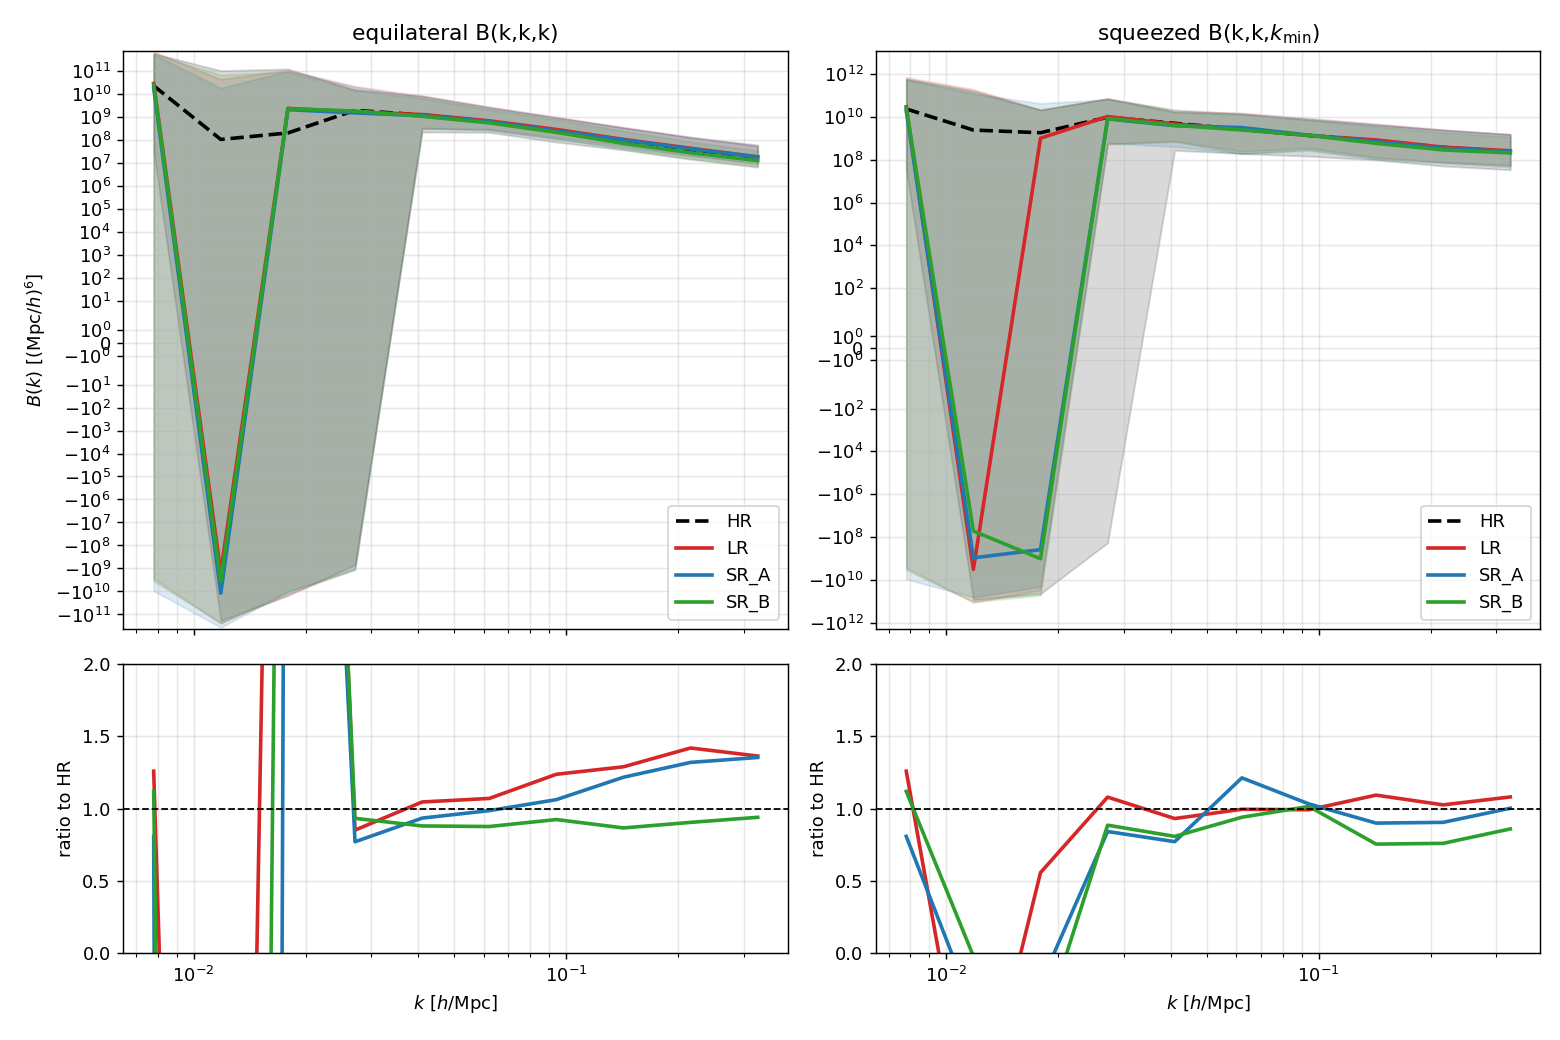
\includegraphics[width=0.95\linewidth]{figures_cmass/bispectrum_hr_lr_srA_srB.png}
\caption{Bispectrum of HR, LR, and SR (both arms), on $16$ test boxes. Top:
equilateral and squeezed bispectrum, HR in black. Bottom: ratio to HR. SR
removes most of the systematic excess that LR has at the plotted scales,
without ever training on this statistic.}
\label{fig:srs-bispec}
\end{figure}

On the equilateral configuration, LR sits about $6$ to $13$ percent above HR
across the middle range of scales. SR removes most of this gap without ever
seeing a bispectrum during training, and it does this for both arms. This is
evidence that the model is not simply fitting the training metric. It is
correcting real structure in the field that also shows up in a statistic it
never saw. (The figure uses the earlier models trained \emph{with} the power
spectrum loss; the no-Pk models of the following paragraphs preserve the
bispectrum at least as well, so removing that loss did not degrade this
held-out statistic either.)

\paragraph{Removing the power spectrum loss.} Following the meeting, we
retrained the model with the power spectrum term switched off
($\lambda_\text{pk}{=}0$ in Eq.~\ref{eq:srs-lossG}), so the loss is only the
adversarial and $L_1$ terms. We also changed which checkpoint counts as "best"
to the real-space $L_1$ error, since selecting on the power spectrum would
have been the same kind of leak we were trying to remove.

\begin{figure}[t]
\centering
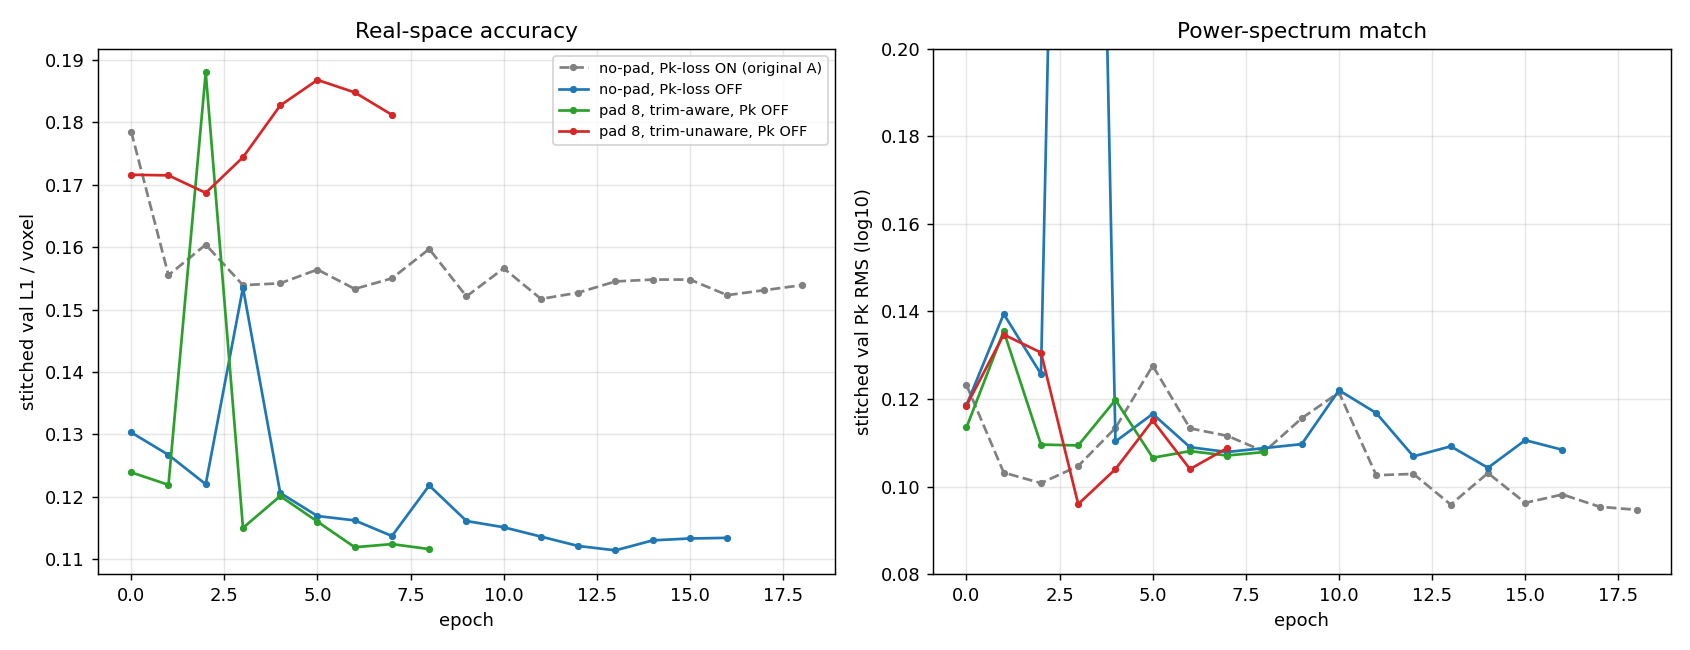
\includegraphics[width=0.98\linewidth]{figures_cmass/protocolv2_cmass.png}
\caption{Stitched validation curves under the new protocol (power spectrum
loss off). Left: real-space $L_1$ error. Right: power spectrum RMS error. Grey
dashed: the original Arm A with the power spectrum loss on, for comparison.
These runs are still training; curves stop at the most recent completed
epoch.}
\label{fig:srs-protocolv2}
\end{figure}

Two things stand out so far. First, without the power spectrum term, the
real-space $L_1$ error becomes clearly better than the original run at the
same point in training (left panel, blue and green curves sit below the grey
dashed curve). Second, the power spectrum error does get a little worse
without its loss term, but it does not collapse: it settles into roughly the
same range as before, just a bit noisier. So the power spectrum term was
buying us a small amount of power spectrum accuracy at a real cost in
real-space accuracy. It was not the only reason the power spectrum matched
well; the adversarial and reconstruction terms carry most of that on their
own.

\paragraph{Does padding help, once the power spectrum loss is out of the way?}
The report above found that padding (Arm B) did not beat no padding (Arm A) on
the power spectrum. The mentor pointed out two different ways this could
happen, and that they make different, testable predictions:
\begin{itemize}
  \item \textbf{Trim-aware.} The model is trained knowing that only the middle
  part of its output will be kept; the loss only looks at that middle part.
  This is what Arm B already did. If this is working correctly, padding should
  train at least as well as no padding, since it has strictly more context for
  the same target.
  \item \textbf{Trim-unaware.} The model is trained as if its whole padded
  output matters, including the edge region that gets thrown away later. If
  the model leans on that edge region during training, it should look fine
  during training but generalize worse once the edge is cut off at test time.
\end{itemize}
We trained both versions with the power spectrum loss off, so the comparison
is not confused by that term. Figure~\ref{fig:srs-protocolv2} shows all three
runs together (no padding, trim-aware padding, trim-unaware padding).

The trim-aware version (green) matches or beats no-padding (blue) on both
real-space error and power spectrum error at almost every epoch measured so
far. This supports the first prediction: once the model is told correctly what
part of its output is graded, more context helps rather than hurts. The
trim-unaware version (red) is clearly worse on real-space error than both
other runs, and does not close that gap as training continues. This supports
the second prediction: a model that is allowed to rely on the part of its
output that gets discarded at test time pays for that at test time. Put
together, the original result that padding did not help was most likely
caused by the power spectrum loss, not by padding itself.

We also reran the older, padding-with-power-spectrum-loss model for more
epochs to check whether it had simply not been trained long enough. Fifteen
additional epochs did not beat its early best score, so that run was not
undertrained; the training recipe, not the training time, was the limiting
factor.

\subsection{The Goal Metric: Corrected Cross-Fidelity Results}
\label{sec:srs-correction}

\paragraph{The bug.} After the analysis above, a routine physical sanity check
failed in a way that could not be real: the amplitude of the power spectrum had
essentially zero correlation with $\sigma_8$, and a fit of the power spectrum to
the five parameters explained only $0.2\%$ of the variance. The power spectrum
amplitude must scale with $\sigma_8$, so this pointed to a labeling error, not to
physics. Tracing it, we found that the processed count fields were written in
string-sorted simulation order ($0, 1, 10, 100, 1000, \dots$) while the cosmology
table is indexed numerically. Field number $k$ is therefore the halo field of
simulation string-sort$(k)$, not simulation $k$, so every field in the whole
pipeline was paired with the wrong cosmology. We proved this exactly: using the
original halo catalogs, the field halo count matches the catalog count under the
string-sort permutation for all $2000$ simulations, while the identity mapping
matches only the two fixed points. We corrected the cosmology table to field
order, backed up the old one, and patched the builder so it cannot regenerate the
wrong order.

\begin{figure}[h]
\centering
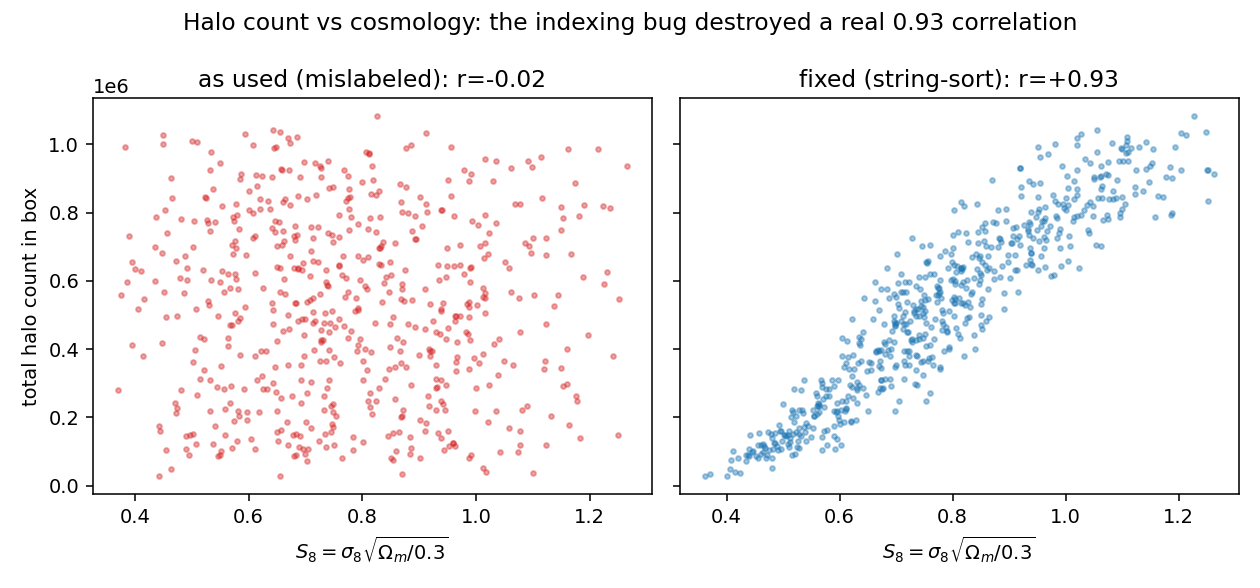
\includegraphics[width=0.85\linewidth]{figures_cmass/labelbug_count_vs_s8.png}
\caption{The indexing bug in one picture. Total halo count in a box against
$S_8 = \sigma_8\sqrt{\Omega_m/0.3}$. As the pipeline used the labels (left) the
correlation is zero; with the string-sort mapping corrected (right) the true
$0.93$ correlation reappears. Halo abundance must track $S_8$, so the left panel
was the signature of a labeling error, not of uninformative data.}
\label{fig:srs-labelbug}
\end{figure}

\paragraph{What this changes, and what it does not.} Every cosmology number we
computed before this point used the labels and is affected; the earlier
cross-fidelity tables have been removed and are replaced by the corrected results
below, and the earlier reading that the SR-versus-LR difference was an irreducible
coin flip was itself a product of the mislabeling. The results that do not use the
labels are unaffected and still stand: the power spectrum match of SR to HR, the
held-out bispectrum, the field-match statistics, the seam test, and the real space
error. The generator conditions on the cosmology as a style vector and was trained
with the scrambled labels, so its conditioning was uninformative during training;
we return to this at the end.

\paragraph{The data is informative after all.} With correct labels the picture
inverts. A halo count in this suite carries a strong cosmological signal: the
total halo count alone correlates with the combination $S_8 = \sigma_8
\sqrt{\Omega_m/0.3}$ at $0.93$ and with $\Omega_m$ at $0.85$. A Fisher forecast on
a single-box power spectrum now explains $98\%$ of the variance, where it
explained $0.2\%$ before, and it constrains $\Omega_m$ and $\sigma_8$ well, with
$\Omega_b$, $h$ and $n_s$ weak or unconstrained, which is the textbook pattern for
a low-redshift halo field. The field-level network tells the same story: after the
fix its predicted $\Omega_m$ correlates with the truth at $0.90$ on both training
and test boxes, where before the fix the correlation was zero and the output was a
constant. So the earlier conclusion that a single box carries almost no cosmology
was an artifact of the labeling, not a property of the data.

\begin{figure}[h]
\centering
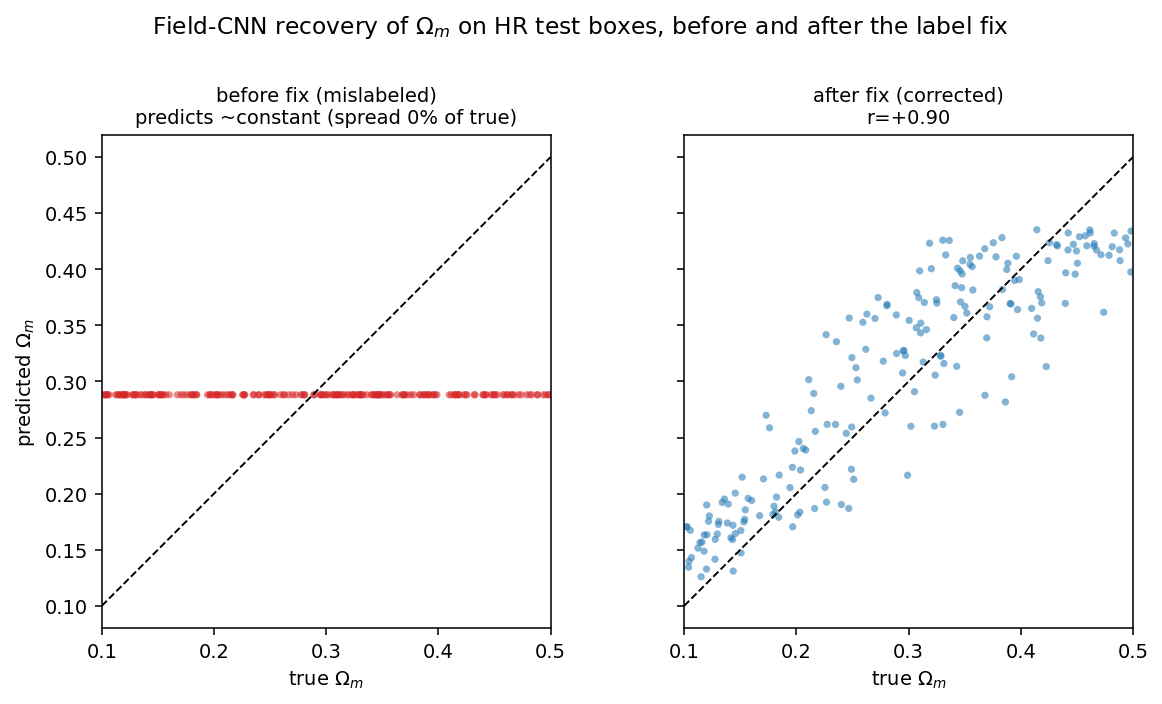
\includegraphics[width=0.82\linewidth]{figures_cmass/field_recovery_Om_cmass.png}
\caption{Field-level CNN recovery of $\Omega_m$ on HR test boxes, before and after
the label fix. Before (left) the prediction is flat and uncorrelated with the
truth (the network returns a near-constant); after (right) it tracks the diagonal
at a correlation of about $0.90$, on both training and test boxes. Same
architecture, same data, only the labels changed.}
\label{fig:srs-recovery}
\end{figure}

\begin{figure}[h]
\centering
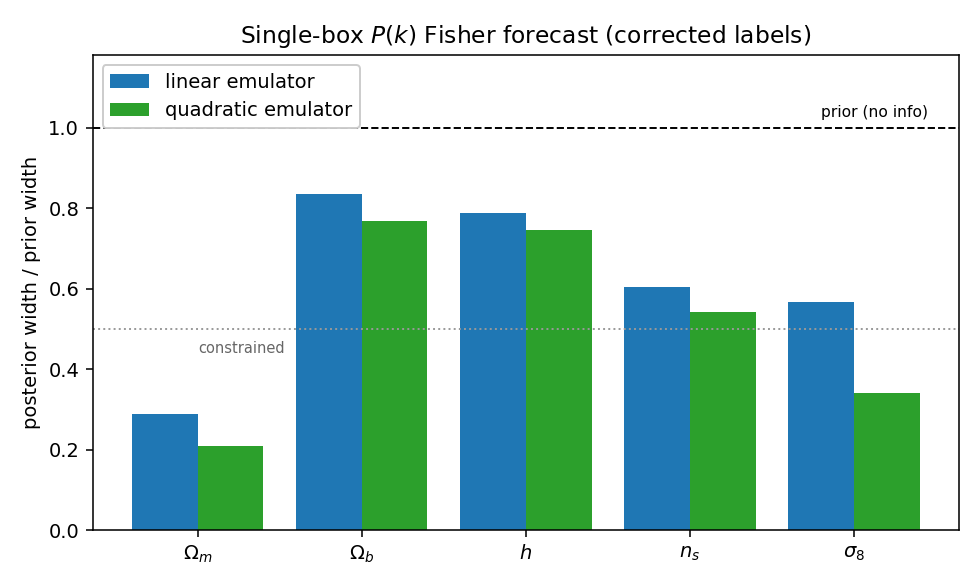
\includegraphics[width=0.72\linewidth]{figures_cmass/fisher_corrected_cmass.png}
\caption{Fisher forecast for a single-box power spectrum with corrected labels:
posterior width divided by prior width per parameter (lower means better
constrained, $1$ means no information). $\Omega_m$ is well constrained and
$\sigma_8$ is constrained, while $\Omega_b$, $h$ and $n_s$ are weak, the textbook
pattern for a low-redshift halo field. Two emulators (linear average slope and
quadratic at the prior centre) bracket the estimate.}
\label{fig:srs-fisher}
\end{figure}

\paragraph{Corrected cross-fidelity, and where SR helps.} We re-ran the goal
metric with correct labels at two levels, the power spectrum summary and the full
field. We train the posterior on one source, apply it to HR, and compare to a
posterior trained on HR, using an ensemble of independently retrained estimators
so the numbers are not single draws. Table~\ref{tab:srs-corrected} gives the
result.
\begin{table}[h]
\centering
\caption{Corrected cross-fidelity KL to HR (posterior trained on the named source,
evaluated on HR), lower is better, with the HR-to-HR floor for reference. Summary
uses the power spectrum; field uses a three-dimensional CNN posterior on the full
box.}
\label{tab:srs-corrected}
\begin{tabular}{lccc}
\toprule
level & LR (raw) & SR & HR floor \\
\midrule
summary $P(k)$ & $0.032$ & $0.088$ & $0.028$ \\
field (CNN)    & $0.49 \pm 0.81$ & $\mathbf{0.024}$ & $0.022$ \\
\bottomrule
\end{tabular}
\end{table}
\begin{figure}[h]
\centering
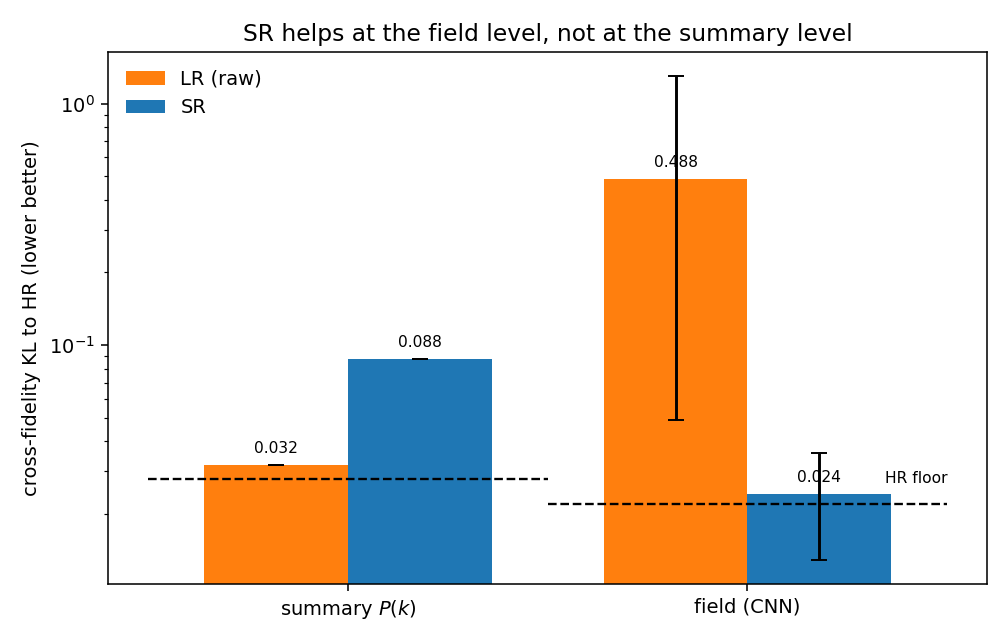
\includegraphics[width=0.7\linewidth]{figures_cmass/crossfid_corrected_cmass.png}
\caption{Corrected cross-fidelity KL to HR (log scale, lower is better) at the two
levels, with the HR-to-HR floor shown as the dashed line. At the summary level the
raw LR field is already at the floor and SR does not help. At the field level, an
LR-trained posterior does not transfer to HR (large and unstable), while an
SR-trained posterior sits at the floor. SR helps exactly where it corrects the
field.}
\label{fig:srs-crossfid-corrected}
\end{figure}
The two levels point in opposite directions, and both make sense. At the summary
level the raw LR power spectrum is already at the HR floor, so an LR-trained
posterior transfers to HR as well as an HR-trained one does, and there is no gap
for SR to close; SR even hurts a little, because the generator reshapes the
small-scale power in a way that does not match how HR responds to cosmology. At
the field level the raw LR box looks different enough from HR that an LR-trained
posterior does not transfer, and it does so unreliably, sometimes acceptably and
sometimes catastrophically, which is why its number carries such a large spread.
SR corrects the field to look like HR, so an SR-trained posterior transfers to HR
reliably, at the floor. This is exactly the deployment case the project is built
on, train the inference model on cheap SR-corrected boxes and apply it to
expensive HR, and at the field level SR makes it work where raw LR does not.

\paragraph{Padding on the goal metric.} We ran the two padding variants through
the corrected cross-fidelity at the summary level as well
(Table~\ref{tab:srs-padding}). Among the SR models the ordering from the earlier
report survives: no padding is best on the goal metric, trim-aware padding is
worse, and trim-unaware is worst, so for the cosmology objective the no-padding
model is the one to use. All three sit above the raw LR control at this level,
consistent with LR already being HR-like on the power spectrum. One number does
change under the fix: the mislabeled data made trim-unaware look catastrophic (a
factor of several hundred above the others), while with correct labels it is the
weakest variant by about a factor of two, not a blow-up. Its real-space error
(Figure~\ref{fig:srs-protocolv2}) remains the clearest and most direct sign that
it is the least reliable model.
\begin{table}[h]
\centering
\caption{Corrected cross-fidelity KL to HR at the summary (power spectrum) level
for the SR padding variants, with the LR control and the HR floor. Lower is
better. Field-level padding numbers are future work.}
\label{tab:srs-padding}
\begin{tabular}{lc}
\toprule
model & summary cross-fidelity KL \\
\midrule
SR, no padding & $\mathbf{0.087}$ \\
SR, trim-aware padding & $0.127$ \\
SR, trim-unaware padding & $0.172$ \\
\midrule
LR (control) & $0.031$ \\
HR floor & $0.028$ \\
\bottomrule
\end{tabular}
\end{table}

\paragraph{Bottom line.} With the labels fixed, the cosmology question has a
clear answer. The data constrains $\Omega_m$ and $\sigma_8$ from a single box. At
the power spectrum level the raw LR field is already HR-like, so SR is not needed
there and slightly hurts. At the field level, which is what SR actually corrects,
an SR-trained posterior transfers to HR at the floor while a raw LR one does not,
so SR provides a real and reliable cosmology benefit exactly where it operates.
Trim-unaware padding is still the weakest variant, worst on the goal metric and
on real-space error, though the label fix shrinks its apparent failure from
catastrophic to about a factor of two. Two honest caveats remain: the
field-level LR number has a wide spread and rests on a handful of retrained
networks, so the size of the gap should be firmed up with more seeds; and because
the generator was trained with the scrambled labels, its cosmology conditioning
was uninformative, so a retrain with correct conditioning may sharpen the SR
result further. Neither caveat changes the direction: with correct labels, SR
helps cosmology at the field level.

\paragraph{A data reliability note.} Partway through these runs, the shared
data storage this project reads from filled up completely, which caused a few
training jobs to fail with a file briefly appearing missing even though it was
not actually deleted. We added a retry step to the data loader and resumed
each affected run from its last saved checkpoint, so no real training progress
was lost. This is a shared infrastructure issue, not a problem with the data or
the method.

\subsection{Files}
\begin{itemize}\itemsep0pt
  \item Data and patching: \texttt{data/patch\_dataset\_cmass.py}
  (shared ops in \texttt{data/patch\_dataset\_real.py})
  \item Model: \texttt{map2map/models/styled\_srsgan.py}
  (\texttt{G\_correct}, \texttt{D\_const})
  \item Training: \texttt{train\_patch\_cmass.py};
  run script \texttt{scripts/train\_patch\_cmass.slurm}
  \item Inference and stitching: \texttt{infer\_stitch\_cmass.py}
  \item Seam eval: \texttt{analysis/eval\_seam\_cmass.py}
  \item Box / per-patch diagnostics: \texttt{analysis/diag\_cmass.py}
  \item SR-vs-HR match stats: \texttt{analysis/match\_stats\_cmass.py}
  \item SR-vs-HR power-spectrum figure: \texttt{analysis/plot\_sr\_vs\_hr.py}
  \item Bispectrum (held-out statistic): \texttt{analysis/bispectrum\_cmass.py}
  \item Training loss curves: \texttt{analysis/plot\_losses\_cmass.py}
  \item Cross-fidelity posterior evaluation: \texttt{evaluate.py} (SR-trained
  or LR-trained posterior evaluated on HR $P(k)$)
  \item Protocol-v2 (no-Pk-loss, padding-variant) training curves:
  \texttt{analysis/plot\_protocolv2\_cmass.py}
  \item Power spectrum on counts: \texttt{analysis/power\_spectrum.py}
  (estimator \texttt{counts}); differentiable training version
  \texttt{analysis/pk\_torch.py}
  \item Posterior and KL: \texttt{inference/nde.py}, \texttt{evaluate.py};
  end-to-end eval \texttt{scripts/eval\_cmass\_wrapper.slurm}
  \item Field-level posterior (three-dimensional CNN, moment-network loss):
  \texttt{models/field\_cnn.py}, \texttt{train\_field\_cnn.py};
  SR field generation \texttt{gen\_sr\_fields.py}; capacity and recovery
  diagnostics \texttt{overfit\_test.py}, \texttt{field\_diag.py}
  \item Outputs: \texttt{runs/patch\_cmass/}; figures: \texttt{figures\_cmass/}
\end{itemize}
 from main.tex, or paste inline.
% Figures referenced live in figures_cmass/ (set \graphicspath or copy them
% next to main.tex). Every number is from runs/patch_cmass/ and FINAL.md.
% =====================================================================

\section{SRS-styled-map2map-galaxy}
\label{sec:srs}

This section documents the second model in this work at the same level of
detail as \S5. Where \S5 corrects a Lagrangian \emph{displacement} field with a
point--voxel flow matcher, this model corrects an Eulerian \emph{halo count}
field with a styled GAN. The two share the same high-level goal, make a cheap
low-fidelity (LF) simulation look like an expensive high-fidelity (HF) one, 
but operate on different data and use a different architecture.

\paragraph{Goal.} Running an accurate (high-resolution) N-body simulation is
expensive; running a fast approximate one is cheap. We want a model that takes
\emph{only} the cheap LF field and produces a corrected field (we call it the
super-resolved or \textbf{SR} field) that matches the expensive HF field. At
inference the model never sees HF: the HF field is used only to train the model
and to grade it. So every result in this section answers one question: \emph{how
close is the SR field, built from LF alone, to the HF field it never saw?}

\paragraph{Terminology.} We work one cubic sub-volume at a time. We call the
$64^3$ output sub-volume a \textbf{core}, and the (possibly larger) input
sub-volume that the model reads a \textbf{patch}. When \texttt{pad}${=}0$ the
patch and the core coincide. We use \textbf{LR}/\textbf{LF} and
\textbf{HR}/\textbf{HF} interchangeably; the data here is named LR (input) and
HR (target).

\paragraph{Two arms.} We test the boundary treatment with two arms that are
identical except for one number:
\begin{itemize}
  \item \textbf{Arm A (naive, mentor 2.1):} \texttt{pad}${=}0$. Each $64^3$ core
  is corrected and placed edge-to-edge.
  \item \textbf{Arm B (overlap, mentor 2.2):} \texttt{pad}${=}8$. Each patch is
  grown to $80^3$ with real neighbour cells (periodic wrap), only the central
  $64^3$ core is kept and placed.
\end{itemize}

\subsection{Data Preprocessing}
\textit{Source: \texttt{cmass-ili}; loader \texttt{data/patch\_dataset\_cmass.py}.}

\paragraph{Input.} We have $2000$ paired simulations at redshift $z=0.5$, run
from shared initial conditions. Each pair is a low-fidelity field (LR, from the
FastPM particle-mesh code) and a high-fidelity field (HR, from a Quijote N-body
run). Both are stored as integer \textbf{halo count grids} of shape
$128\times128\times128$ on a periodic box of side $L_\text{box}=1000\
\mathrm{Mpc}/h$ (cell size $\approx 7.81\ \mathrm{Mpc}/h$). A cell value is the
number of halos whose position falls in that cell. The fields are sparse: most
cells are zero and the mean count per cell is small (the code caches one global
count scale, the mean HR count per cell measured over $50$ training sims).
Because LR and HR share initial conditions, they describe the same structure at
two fidelities. The correspondence is between the two halo catalogs \emph{as a
whole}: there is no known one-to-one matching between individual LR and HR
halos, only between the count fields they produce.

\paragraph{Cosmology labels.} Each simulation carries a style vector
$\mathbf s=(\Omega_m,\Omega_b,h,n_s,\sigma_8)\in\mathbb R^5$, parsed from that
sim's \texttt{config.yaml}.

\paragraph{Splits.} The on-disk lists give $1600$ train, $200$ validation, and
$200$ test simulations, split by simulation index.

\begin{figure}[t]
\centering
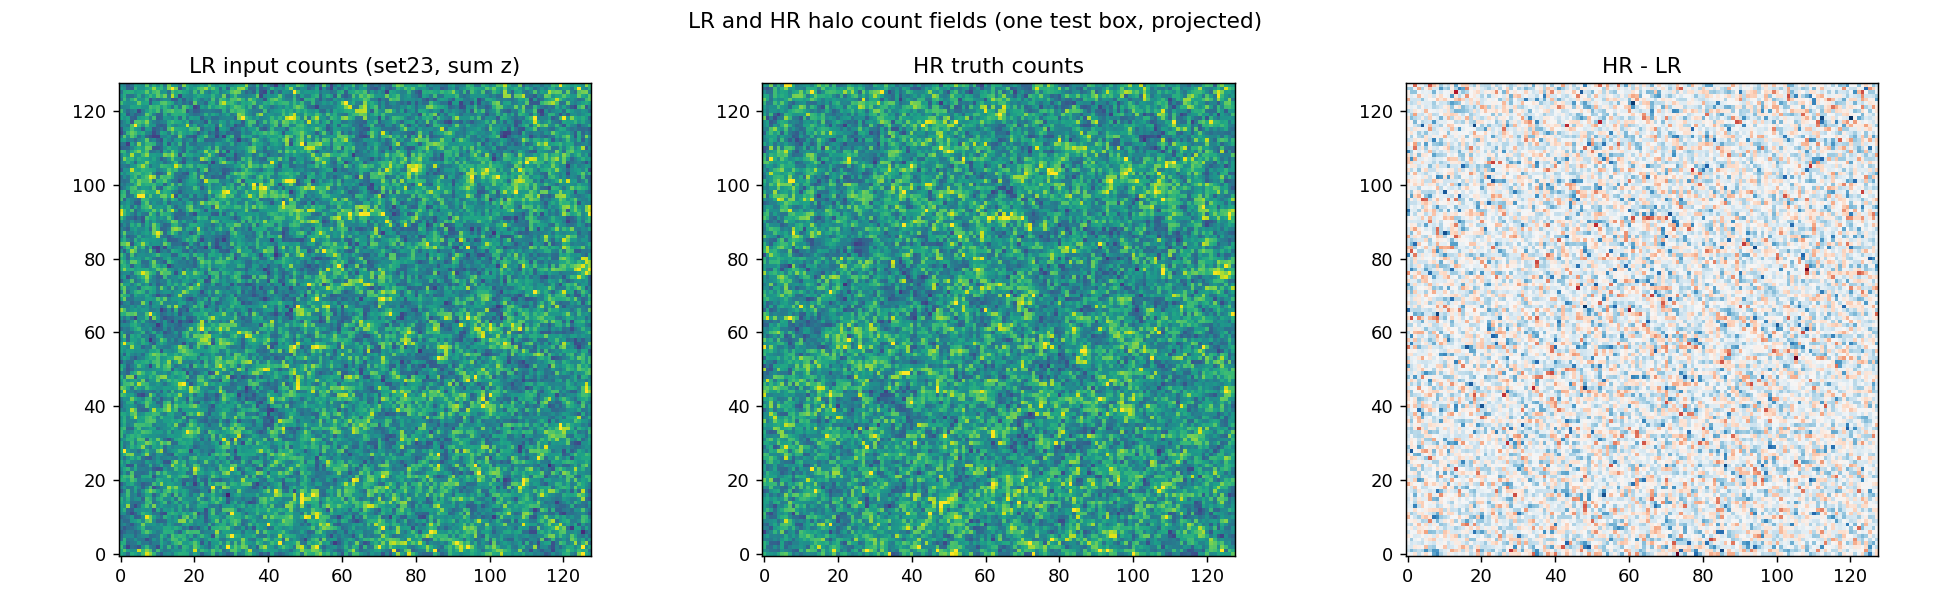
\includegraphics[width=0.9\linewidth]{figures_cmass/data_pair.png}
\caption{One LR/HR pair (projected count map). LR (FastPM, input) and HR
(Quijote N-body, target) share initial conditions and so share large-scale
structure, but differ cell-by-cell.}
\label{fig:srs-datapair}
\end{figure}

\paragraph{Model space (count transform).} The network does not learn on raw
counts; it learns in a compressed ``model space''. The default transform is
$\log(1+n)$, which tames the sparse heavy tail:
\begin{equation}
  y = \log(1+n), \qquad n = \exp(y)-1 \ \ (\text{clamped to } n\ge 0).
  \label{eq:srs-transform}
\end{equation}
Two alternative transforms exist in the code (\texttt{scale}: $n/\text{scale}$;
\texttt{delta}: model space is the overdensity itself), but all reported runs use
$\log(1+n)$. Power spectra are \emph{never} computed in model space; they are
always computed on the physical-count overdensity \SG{Is it okay if this is -1 when there are 0 halos?}
\begin{equation}
  \delta = \frac{n}{\bar n} - 1,
  \label{eq:srs-delta}
\end{equation}
with $\bar n$ the per-box mean count (the \texttt{perbox} setting used in all
runs).

\subsection{Data Pipeline (patching)}
\textit{Located in: \texttt{data/patch\_dataset\_cmass.py},
\texttt{data/patch\_dataset\_real.py} (shared patch ops).}

A model never sees the whole $128^3$ box at once. We cut the box into a
$2\times2\times2$ grid of $64^3$ \textbf{cores} (Table~\ref{tab:srs-notation}).
The cores tile the box exactly (stride $64$), so they reconstruct the box
bit-for-bit with no gaps and no double counting, the dataset's self-test
asserts this. Each model \emph{input} is a core grown by \texttt{pad} voxels on
every side, taken from the true neighbour cells with periodic wrap at the box
edge (\texttt{extract\_patch} uses \texttt{numpy.take(\dots, mode="wrap")}). So
with \texttt{pad}${=}8$ the input is $80^3$ and neighbouring patches overlap by
$2\cdot\texttt{pad}=16$ voxels; the HR \emph{target} is always the bare $64^3$
core. Because each simulation is one continuous periodic box that we crop
ourselves, the patches are real neighbours by construction, there is no data
seam (unlike the Lagrangian patches of \S5). \SG{Isn't the patch construction same in both?}

\begin{table}[t]
\centering
\caption{Notation for the CMASS count-field pipeline.}
\label{tab:srs-notation}
\begin{tabular}{llp{7.2cm}}
\toprule
Symbol & Value & Meaning \\
\midrule
$N_\text{full}$    & $128$ & full box side (voxels) \\
$P$ (\texttt{PATCH}) & $64$ & core side (voxels) \\
$N_\text{patches}$ & $8$ & cores per box ($2{\times}2{\times}2$) \\
\texttt{pad}       & $0$ (Arm A) / $8$ (Arm B) & halo width added to each face by periodic wrap \\
$L_\text{box}$     & $1000\ \mathrm{Mpc}/h$ & box side \\
$\mathbf s$        & $\in\mathbb R^5$ & cosmology vector $(\Omega_m,\Omega_b,h,n_s,\sigma_8)$ \\
$\bar n$           & per-box mean & mean count used to form $\delta=n/\bar n-1$ \\
\bottomrule
\end{tabular}
\end{table}

\begin{figure}[t]
\centering
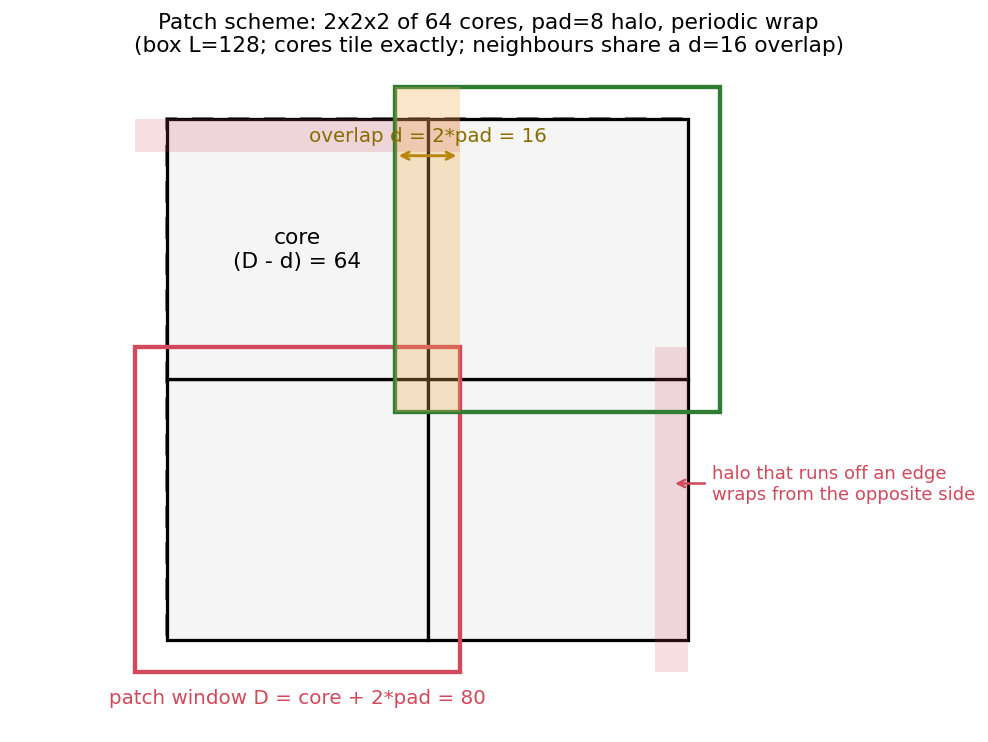
\includegraphics[width=0.82\linewidth]{figures_cmass/pipeline_patching.png}
\caption{Patch scheme. The box is cut into a $2{\times}2{\times}2$ grid of
$64^3$ cores that tile it exactly. With \texttt{pad}${>}0$ each patch is grown by
a halo of real neighbour cells (periodic wrap); only the central core is kept
and placed back.}
\label{fig:srs-patching}
\end{figure}

\paragraph{Per-simulation item.} Indexed by simulation, the dataset returns, for
all $8$ cores at once: the LR patches \texttt{lr\_in} of shape
$(8,\,1,\,64{+}2\,\texttt{pad},\,\cdot,\,\cdot)$ in model space, the HR cores
\texttt{hr\_tgt} of shape $(8,\,1,\,64,\,64,\,64)$, the style $\mathbf s$, and
the simulation index. The trainer flattens the $8$-core axis into the batch.

\begin{algorithm}[H]
\caption{\textsc{ExtractPatches} (one simulation)}
\label{alg:srs-extract}
\begin{algorithmic}[1]
\Require LR box $\mathbf L\in\mathbb R^{1\times128^3}$, HR box $\mathbf H$, \texttt{pad}
\State map $\mathbf L,\mathbf H$ to model space via Eq.~\ref{eq:srs-transform}
\For{$p=0,\dots,7$}
  \State $(i,j,k)\gets\textsc{unravel}(p,(2,2,2))$ \Comment{core origin $(64i,64j,64k)$}
  \State $\mathbf L_p\gets$ core $p$ grown by \texttt{pad} on each face, periodic wrap \Comment{$(64{+}2\,\texttt{pad})^3$}
  \State $\mathbf H_p\gets$ bare core $p$ \Comment{$64^3$}
\EndFor
\State \Return $\{(\mathbf L_p,\mathbf H_p)\}_{p=0}^{7}$, style $\mathbf s$
\end{algorithmic}
\end{algorithm}

\subsection{Model: Input/Output Specification}
\textit{Implementation: \texttt{map2map/models/styled\_srsgan.py}
(\texttt{G\_correct}, \texttt{D\_const}).}

\paragraph{What the generator computes.} The generator is a
\textbf{same-resolution residual} network: it does not change the grid size, and
it predicts a correction that is \emph{added} to the input. In model space,
\begin{equation}
  \mathrm{SR} \;=\; \mathrm{LR} \;+\; G(\mathrm{LR},\,\mathbf s,\,\mathbf z),
  \label{eq:srs-residual}
\end{equation}
where $\mathbf s$ is the cosmology vector and $\mathbf z$ is an injected noise
field (see below). Inputs and outputs are listed in
Table~\ref{tab:srs-model-io}; the generator is run once per core (the $8$ cores
of a box form a batch).

\begin{table}[t]
\centering
\caption{Tensors consumed/produced by the generator \texttt{G\_correct} for one
core (batch dimension omitted). Here $D=64{+}2\,\texttt{pad}$.}
\label{tab:srs-model-io}
\begin{tabular}{lll}
\toprule
Symbol & Shape & Meaning \\
\midrule
$\mathbf x$ (\texttt{x})       & $(1,D,D,D)$ & LR patch, model space (input) \\
$\mathbf s$ (\texttt{style})   & $(5,)$      & cosmology vector \\
$\mathbf z$ (\texttt{noise\_list}) & $2\cdot\texttt{num\_blocks}$ cubes $(1,D,D,D)$ & injected noise; fixed at inference, random in training \\
$G(\cdot)$                     & $(1,D,D,D)$ & predicted residual $\delta$ (added to $\mathbf x$) \\
\bottomrule
\end{tabular}
\end{table}

\paragraph{Internal composition.} $G$ is a constant-resolution StyleGAN2-style
network (no up/down-sampling), built from:
\begin{enumerate}
  \item \texttt{block0}: a $1{\times}1{\times}1$ style-modulated convolution
  (\texttt{ConvStyled3d}) lifting the $1$-channel input to $c_0$ channels,
  followed by a leaky ReLU.
  \item \texttt{num\_blocks} ($=4$) constant-resolution H-blocks
  (\texttt{HBlock\_const}). Each block, in order: inject noise $\to$
  $3{\times}3{\times}3$ \texttt{ConvStyled3d} (periodic ``circular'' padding)
  $\to$ leaky ReLU $\to$ inject noise $\to$ $3{\times}3{\times}3$
  \texttt{ConvStyled3d} $\to$ leaky ReLU $\to$ a $1{\times}1{\times}1$ projection
  to the output channel, accumulated into a running output $y$. The final return
  is $\mathbf x + y$ (Eq.~\ref{eq:srs-residual}).
\end{enumerate}
The channel widths come from \texttt{chan\_base} ($=128$) halved per block and
clamped to $[64,512]$. Two mechanisms make the convolutions depend on side
information:
\begin{itemize}
  \item \textbf{Style modulation.} \texttt{ConvStyled3d} is the StyleGAN2
  modulated/demodulated convolution: the cosmology vector $\mathbf s$ scales the
  convolution weights, so the same network behaves differently for different
  cosmologies. This is the only path by which $\mathbf s$ enters.
  \item \textbf{Noise injection.} Each \texttt{ConvStyled3d} is preceded by a
  per-channel learned-standard-deviation noise add (\texttt{\_NoiseInject}). At
  training time the noise is fresh Gaussian each call; at inference a
  \emph{fixed} list of noise cubes (seeded, built by \texttt{build\_noise\_list})
  is reused so outputs are reproducible. The noise is what lets the model produce
  a plausible small-scale field rather than a single blurred guess.
\end{itemize}

\paragraph{Discriminator.} \texttt{D\_const} is a constant-input-resolution
critic conditioned on the same style $\mathbf s$. It runs a head
\texttt{ConvStyled3d} then \texttt{num\_blocks} strided down-blocks (each a
periodic $3{\times}3{\times}3$ \texttt{ConvStyled3d} $+$ leaky ReLU $+$
$2{\times}$ average pool), a $1{\times}1{\times}1$ tail, and a final
$1{\times}1{\times}1$ projection to one channel, averaged over space to a single
logit per core.

\subsection{Training Step}
\textit{Located in: \texttt{train\_patch\_cmass.py}.}

The generator is trained per core (stitching is \emph{not} part of the
gradient). The total generator loss is a weighted sum of three terms,
\begin{equation}
  \mathcal L_G \;=\; \lambda_\text{adv}\,\mathcal L_\text{adv}
                  + \lambda_\text{rec}\,\mathcal L_\text{rec}
                  + \lambda_\text{pk}\,\mathcal L_\text{pk},
  \label{eq:srs-lossG}
\end{equation}
with (defaults from the original run script; see the protocol update below for
the values now in use):
\begin{itemize}
  \item \textbf{Reconstruction} $\mathcal L_\text{rec}=\lVert \mathrm{SR}-\mathrm{HR}\rVert_1$,
  a plain $L_1$ in model space (optionally Gaussian-smoothed; smoothing off in
  all runs).
  \item \textbf{Power-spectrum} $\mathcal L_\text{pk}$, the mean-squared error
  between the $\log_{10}$ power spectra of SR and HR, computed on the
  \emph{physical-count overdensity} of the $64^3$ core (Eqs.~\ref{eq:srs-transform}--\ref{eq:srs-delta}),
  Hann-windowed, with the HR side detached:
  \begin{equation}
    \mathcal L_\text{pk} = \frac{1}{|K|}\sum_{k\in K}
      \big(\log_{10} P_\text{SR}(k) - \log_{10} P_\text{HR}(k)\big)^2 .
    \label{eq:srs-pkloss}
  \end{equation}
  \item \textbf{Adversarial} $\mathcal L_\text{adv}=\mathrm{softplus}\!\big({-}D(\mathrm{SR},\mathbf s)\big)$,
  the non-saturating GAN generator loss.
\end{itemize}

\paragraph{Protocol update: what region the reconstruction and adversarial
terms see.} A \texttt{--pad-loss} setting controls how much of the generator's
output the $L_1$ and adversarial terms are computed on, independent of
\texttt{pad} itself:
\begin{itemize}
  \item \texttt{crop} (trim-aware, the setting used for Arm B above): the loss
  is computed only on \textsc{cropInterior}$(G(\mathbf x,\mathbf s),\,\texttt{pad})$,
  the $64^3$ core that is actually kept at inference time, against the bare
  $64^3$ HR core. The model is trained on exactly the region it will be graded
  on.
  \item \texttt{full}: the loss is computed on the whole $(64{+}2\,\texttt{pad})^3$
  output, against a correspondingly padded HR target (the dataset's
  \texttt{pad\_target} option). The model is trained as if the halo region it
  will later be trimmed off also mattered.
\end{itemize}
Concretely, let $\texttt{loss\_crop}=\texttt{pad}$ under \texttt{crop} and $0$
under \texttt{full}; every place above that writes $\mathrm{SR}$ means
$\textsc{cropInterior}(G(\mathbf x,\mathbf s),\,\texttt{loss\_crop})$, and the
Hann window and $P(k)$ estimator in $\mathcal L_\text{pk}$ are sized to match.
This is a controlled test of two ways padding could fail to help: see the
protocol-update subsection below for the result.

The discriminator is trained with the non-saturating GAN loss plus a lazy $R_1$
gradient penalty applied every \texttt{r1\_every} steps:
\begin{equation}
  \mathcal L_D = \mathrm{softplus}\!\big({-}D(\mathrm{HR})\big)
               + \mathrm{softplus}\!\big(D(\mathrm{SR})\big)
               + \tfrac{1}{2}\lambda_{R_1}\,\mathbb E\big\lVert \nabla_{\!x} D(x,\mathbf s)\big\rVert^2 .
  \label{eq:srs-lossD}
\end{equation}

\begin{algorithm}[H]
\caption{CMASS patch-GAN training step (one batch of cores)}
\label{alg:srs-train}
\begin{algorithmic}[1]
\Require LR patches $\mathbf x$, HR targets $\mathbf h$ (padded iff \texttt{pad-loss=full}),
         style $\mathbf s$, \texttt{pad}, \texttt{loss\_crop} ($=\texttt{pad}$ if \texttt{crop} else $0$),
         weights $\lambda_\text{adv},\lambda_\text{rec},\lambda_\text{pk},\lambda_{R_1}$
\Statex \textbf{// Discriminator}
\State $\hat{\mathbf h}\gets \textsc{cropInterior}\big(G(\mathbf x,\mathbf s),\,\texttt{loss\_crop}\big)$ \Comment{no grad}
\State $\mathcal L_D \gets \mathrm{softplus}({-}D(\mathbf h,\mathbf s)) + \mathrm{softplus}(D(\hat{\mathbf h},\mathbf s))$
\If{step $\bmod\ \texttt{r1\_every} = 0$} $\mathcal L_D \mathrel{+}= \tfrac12\lambda_{R_1}\texttt{r1\_every}\cdot R_1(D,\mathbf h,\mathbf s)$ \EndIf
\State update $D$ (Adam, grad-clip)
\Statex \textbf{// Generator}
\State $\hat{\mathbf h}\gets \textsc{cropInterior}\big(G(\mathbf x,\mathbf s),\,\texttt{loss\_crop}\big)$
\State $\mathcal L_\text{adv}\gets \mathrm{softplus}({-}D(\hat{\mathbf h},\mathbf s))$
\State $\mathcal L_\text{rec}\gets \lVert \hat{\mathbf h}-\mathbf h\rVert_1$
\State $\mathcal L_\text{pk}\gets$ Eq.~\ref{eq:srs-pkloss} on Hann-windowed overdensity of $\hat{\mathbf h}$, $\mathbf h$
       (skip if $\lambda_\text{pk}{=}0$)
\State $\mathcal L_G \gets \lambda_\text{adv}\mathcal L_\text{adv}+\lambda_\text{rec}\mathcal L_\text{rec}+\lambda_\text{pk}\mathcal L_\text{pk}$
\State update $G$ (Adam, grad-clip)
\end{algorithmic}
\end{algorithm}

\paragraph{Validation and checkpoint selection.} After each epoch we stitch the
full $128^3$ SR box for up to $40$ validation sims and report the stitched
$L_1$/voxel and the stitched-$128$ power-spectrum RMS against HR
(\S\ref{sec:srs-eval}, Eq.~\ref{eq:srs-pkrms}). A \texttt{--select} setting
chooses which of the two the saved \texttt{best.pt} tracks: \texttt{pk} (the
original setting, lowest stitched validation Pk RMS) or \texttt{l1} (lowest
stitched validation $L_1$/voxel). Selection is always on the stitched full box,
not the per-core training loss. Runs that also train with $\lambda_\text{pk}{=}0$
use \texttt{--select l1}, since selecting on Pk RMS while not training on it
would reintroduce the same metric leak in a different place.

\subsection{Inference}
\textit{Located in: \texttt{infer\_stitch\_cmass.py}.}

For one simulation: load the LR $128^3$ count box, map it to model space, run $G$
on each of the $8$ cores (with the periodic-wrap halo in Arm B), crop the halo,
stitch the cores into a $128^3$ model-space box, invert the transform to physical
counts, and clamp. \SG{are all outputs later mapped to integers, or are we fine with non-integer number of halos?} The injected noise list is fixed (seeded) so the output is
reproducible.

\begin{algorithm}[H]
\caption{CMASS inference + stitch (one simulation)}
\label{alg:srs-infer}
\begin{algorithmic}[1]
\Require LR box $\mathbf L$, style $\mathbf s$, trained $G$, mode (naive/overlap), fixed noise $\mathbf z$
\State $\texttt{pad}\gets 0$ if naive else value from checkpoint ($8$)
\State map $\mathbf L$ to model space (Eq.~\ref{eq:srs-transform})
\For{$p=0,\dots,7$}
  \State $\mathbf x_p\gets$ patch $p$ (core grown by \texttt{pad}, periodic wrap)
  \State $\mathbf c_p\gets \textsc{cropInterior}\big(G(\mathbf x_p,\mathbf s,\mathbf z),\,\texttt{pad}\big)$ \Comment{$64^3$ core, model space}
\EndFor
\State $\mathbf S\gets \textsc{stitch}(\{\mathbf c_p\})$ \Comment{$128^3$, model space}
\State $\mathbf S\gets \exp(\mathbf S)-1$, clamp to $[0,\,C_\text{max}{=}200]$, replace NaN/Inf \Comment{physical counts}
\State \Return $\mathbf S$
\end{algorithmic}
\end{algorithm}

\subsection{Crop Stitching}

Stitching is \textbf{direct placement with no averaging}. Adjacent cores tile the
box exactly (stride $64$, no overlap between cores once the halo is dropped), so
each core's $64^3$ output is written straight into its slot. In Arm B the $80^3$
patch is corrected and only its central $64^3$ core is kept; the overlap halo is
context for the convolution, never written to the output.

\begin{algorithm}[H]
\caption{\textsc{Stitch} ($8$ cores $\to$ $128^3$)}
\label{alg:srs-stitch}
\begin{algorithmic}[1]
\Require cores $\{\mathbf c_p\}_{p=0}^{7}$, each $1\times64^3$
\State $\mathbf S\gets \mathbf 0\in\mathbb R^{1\times128^3}$
\For{$p=0,\dots,7$}
  \State $(i,j,k)\gets\textsc{unravel}(p,(2,2,2))$
  \State $\mathbf S[:,\,64i{:}64i{+}64,\,64j{:}\cdots,\,64k{:}\cdots]\gets \mathbf c_p$ \Comment{direct assignment}
\EndFor
\State \Return $\mathbf S$
\end{algorithmic}
\end{algorithm}

\subsection{Evaluation}
\label{sec:srs-eval}
\textit{Located in: \texttt{analysis/eval\_seam\_cmass.py},
\texttt{analysis/diag\_cmass.py}, \texttt{analysis/match\_stats\_cmass.py},
\texttt{analysis/power\_spectrum.py}, \texttt{inference/nde.py},
\texttt{evaluate.py}.}

We evaluate the SR field against HR at three levels: a seam check (does stitching
leave a join?), field statistics (does SR have the right structure?), and
cosmology (does SR give the same parameter posterior as HR?).

\paragraph{Power-spectrum summaries.} On the count overdensity (Eq.~\ref{eq:srs-delta})
we report the power spectrum $P(k)$, the transfer ratio, and the cross-coherence:
\begin{equation}
  T(k) = \frac{P_\text{SR}(k)}{P_\text{HR}(k)},
  \qquad
  r(k) = \frac{P_{\text{SR},\text{HR}}(k)}{\sqrt{P_\text{SR}(k)\,P_\text{HR}(k)}} .
  \label{eq:srs-Tr}
\end{equation}
$T(k)=1$ means SR has the right \emph{amount} of power at scale $k$ (amplitude);
$r(k)=1$ means SR has the structure in the right \emph{place} (phase). The
scalar power-spectrum error used for checkpoint selection and seam reporting is
the log-RMS over the resolved $k$-bins:
\begin{equation}
  \mathrm{PkRMS}_{\log_{10}} = \sqrt{\frac{1}{|K|}\sum_{k\in K}
    \big(\log_{10} P_\text{SR}(k) - \log_{10} P_\text{HR}(k)\big)^2 } .
  \label{eq:srs-pkrms}
\end{equation}

\paragraph{Seam diagnostic.} \texttt{eval\_seam\_cmass.py} bins the per-cell
count error $|{\mathrm{SR}-\mathrm{HR}}|$ by distance to the nearest core face
and forms a per-position error profile along each axis. The headline number is
the \textbf{$x{=}64$ internal-seam excess}: the error on the internal core
boundary plane divided by the interior error. A value near $1$ means stitching
leaves no seam. The box edge $x{=}0$ is a periodic-boundary control.

\paragraph{Field-match statistics.} \texttt{match\_stats\_cmass.py} reports, over
$16$ test boxes: the total-count ratio $\sum\mathrm{SR}/\sum\mathrm{HR}$, the
void fraction (cells $<0.5$), the real-space cell standard-deviation ratio
$\mathrm{std}(\mathrm{SR})/\mathrm{std}(\mathrm{HR})$ (a blur check), and the
cross-coherence $r(k)$ at large ($k<0.05$) and small ($k>0.2$) scales.

\paragraph{Cosmology (posterior consistency).} This is the strongest ``does SR
match HR'' test. We voxel-count $\to$ overdensity $\to$ $P(k)$ for every box, then
train a neural density estimator $q(\theta\mid P(k))$ on the training split using
\texttt{sbi} (\texttt{SNPE\_C} with a neural-spline-flow density estimator,
\texttt{inference/nde.py}); the summary is $\log_{10}P(k)$. We train one estimator
on HR ($q_\text{HR}$) and one on each SR arm ($q_\text{SR}$). For each test box we
draw $2000$ posterior samples from each, fit a Gaussian per parameter, and report
the per-parameter Gaussian KL (\texttt{evaluate.py}):
\begin{equation}
  \mathrm{KL}\big(\mathcal N(\mu_\text{HR},\sigma_\text{HR})\,\Vert\,\mathcal N(\mu_\text{SR},\sigma_\text{SR})\big)
  = \tfrac12\!\left[\log\frac{\sigma_\text{SR}^2}{\sigma_\text{HR}^2}
    + \frac{\sigma_\text{HR}^2+(\mu_\text{HR}-\mu_\text{SR})^2}{\sigma_\text{SR}^2} - 1\right].
  \label{eq:srs-kl}
\end{equation}
$\mathrm{KL}=0$ means SR gives the identical cosmology posterior to HR. The raw LR
field (no model), pushed through the same pipeline, is the control SR must beat.

We report this comparison in two forms, and it matters which is which:
\begin{itemize}
  \item \textbf{Cross-fidelity (primary).} $q_\text{SR}$ is trained on SR power
  spectra but \emph{evaluated on the HR} $P(k)$ of each test simulation, and
  compared to $q_\text{HR}$ evaluated on the same HR $P(k)$. This is the
  deployment scenario the project targets: HR simulations are too expensive to
  train an inference model on, so the inference model is trained on cheap SR
  output and must still work when applied to (HR-like) reality. The comparison
  against an LR-trained estimator on the same HR data measures whether sampling
  in HR space (SR) survives the distribution shift better than staying in LR
  space. This metric never appears in the training loss.
  \item \textbf{Own-data (secondary).} $q_\text{SR}$ trained and evaluated on SR
  vs $q_\text{HR}$ trained and evaluated on HR, each pipeline end-to-end on
  its own field type.
\end{itemize}

\subsection{Best-Run Configuration}
\textit{Run script: \texttt{scripts/train\_patch\_cmass.slurm}; checkpoints
\texttt{checkpoints/patch\_cmass\_\{A,B\}/best.pt}.}

Both arms use the identical configuration below; they differ only in \texttt{pad}
($0$ for Arm~A, $8$ for Arm~B). This is the configuration behind every number
in \S\ref{sec:srs-results}--\S\ref{sec:srs-next}.

\begin{lstlisting}[language=bash]
--transform log1p   --nbar perbox        # log(1+n) model space; per-box nbar
--epochs 30         --sims-per-batch 1    # patch-batch = 8 cores per step
--chan-base-g 128   --chan-base-d 64  --num-blocks 4
--lambda-adv 1.0    --lambda-rec 2.0  --lambda-pk 2.0   # generator weights
--lambda-r1 10.0    --r1-every 16                       # lazy R1
--lr-g 1e-4 --lr-d 1e-4  --beta1 0.0 --beta2 0.99       # Adam
--grad-clip 1.0     --val-max-sims 40    --select pk    # select on Pk RMS
\end{lstlisting}

The best checkpoint per arm is the one with the lowest stitched validation Pk RMS
(Eq.~\ref{eq:srs-pkrms}):

\begin{center}
\begin{tabular}{lc}
\toprule
arm & best stitched val PkRMS$_{\log_{10}}$ \\
\midrule
Arm A, naive (pad $0$)  & $0.0947$ \\
Arm B, overlap (pad $8$) & $0.0963$ \\
\bottomrule
\end{tabular}
\end{center}

\paragraph{Protocol update.} Following the mentor meeting reported in
\S\ref{sec:srs-followup}, the configuration above is no longer the one we train
with. Three settings changed:
\begin{lstlisting}[language=bash]
--lambda-pk 0.0      # power-spectrum term OFF (it was also our main metric)
--pad-loss crop|full # trim-aware vs trim-unaware padding, see below
--select l1          # select on stitched L1, not the term we removed
\end{lstlisting}
All results in \S\ref{sec:srs-followup} use this configuration. Runs under the
original configuration above (Arm A, Arm B, and everything derived from them in
\S\ref{sec:srs-results}--\S\ref{sec:srs-next}) remain valid as a record of that
protocol; they are superseded, not invalidated, by the update.

\subsection{Results: Does SR Match HR?}
\label{sec:srs-results}

All numbers are on the $200$-box test split unless noted.

\paragraph{1. Power spectrum (statistics).} Across the test set the SR power
spectrum tracks HR at every scale, and Arm A beats the no-model LR control on the
overall log-RMS (Fig.~\ref{fig:srs-srvshr}, computed by
\texttt{analysis/plot\_sr\_vs\_hr.py}).

\begin{table}[h]
\centering
\caption{SR vs HR power-spectrum agreement, $200$ test boxes. Transfer
$T(k)=P_X/P_\text{HR}$ (Eq.~\ref{eq:srs-Tr}); $1.0$ is perfect.}
\label{tab:srs-pk}
\begin{tabular}{lccc}
\toprule
field (vs HR) & PkRMS$_{\log_{10}}$ & $T$ at large scales ($k{<}0.1$) & $T$ at small scales ($k{>}0.3$) \\
\midrule
SR (Arm A, naive)    & $\mathbf{0.0607}$ & $0.95$ & $1.04$ \\
SR (Arm B, overlap)  & $0.0645$ & $0.93$ & $0.88$ \\
LR (no model, control) & $0.0641$ & $1.01$ & $1.01$ \\
\bottomrule
\end{tabular}
\end{table}

\begin{figure}[t]
\centering
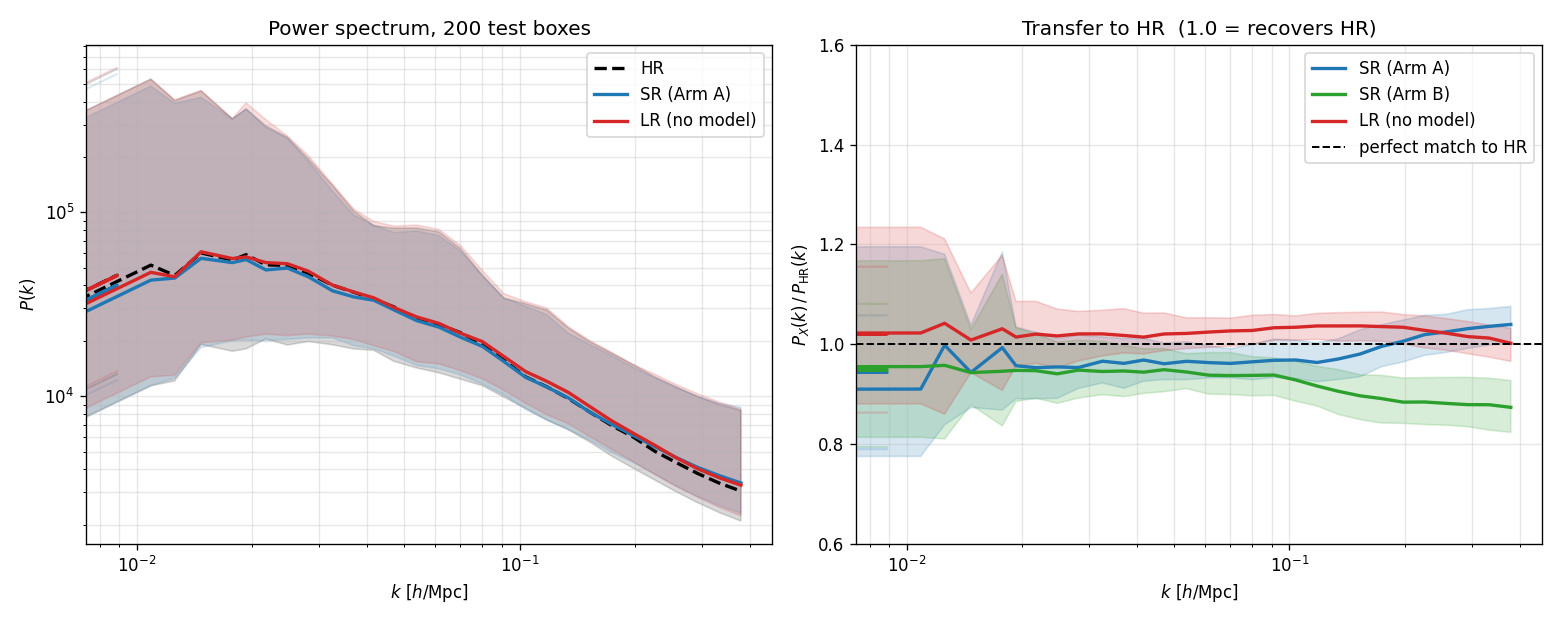
\includegraphics[width=0.98\linewidth]{figures_cmass/sr_vs_hr_pk.png}
\caption{\textbf{Left:} $P(k)$ of HR, SR (Arm A), and LR over $200$ test boxes
(median $+$ $16/84\%$ band). \textbf{Right:} transfer to HR; $1.0$ recovers HR.
SR (Arm A) sits near $1$ at all scales; Arm B's overlap blending slightly
suppresses small-scale power (transfer $0.88$).}
\label{fig:srs-srvshr}
\end{figure}

\paragraph{2. Field structure.} Beyond the power spectrum, SR keeps the field
structure of HR (Arm A, $16$ test boxes, \texttt{match\_stats\_cmassA.txt}):

\begin{table}[h]
\centering
\caption{SR vs HR field-match statistics (Arm A).}
\label{tab:srs-match}
\begin{tabular}{lll}
\toprule
quantity & value & reading \\
\midrule
total count ratio $\sum\mathrm{SR}/\sum\mathrm{HR}$ & $0.965\pm0.172$ & counts conserved on average; large per-box scatter \\
real-space std ratio & $1.008\pm0.100$ & clustering amplitude matches; not blurred \\
void fraction SR / HR ($<0.5$) & $0.855$ / $0.833$ & SR keeps voids empty, like HR \\
cross-coherence $r$, $k<0.05$ & $0.951$ & large-scale structure matches cell-by-cell \\
cross-coherence $r$, $k>0.2$ & $0.403$ & small-scale structure decorrelates \\
\bottomrule
\end{tabular}
\end{table}

\paragraph{3. Cosmology.} The cosmology comparison in the original report used
mislabeled cosmologies, an indexing bug we describe and fix in
\S\ref{sec:srs-correction}, so those numbers are not shown here. With correct
labels a single box constrains $\Omega_m$ and $\sigma_8$; at the power spectrum
level the raw LR field is already HR-like, while at the field level an SR-trained
posterior transfers to HR and an LR-trained one does not
(\S\ref{sec:srs-correction}, Table~\ref{tab:srs-corrected}).

\paragraph{4. Seam.} Neither arm introduces a stitching seam: the $x{=}64$
internal-seam excess is $\approx1$ for both
(Table~\ref{tab:srs-seam}, Fig.~\ref{fig:srs-seam}). Arm A shows a mild generic
ripple near \emph{any} boundary plane (seam-distance ratio $1.17$); Arm B's
overlap removes it ($1.00$) at a small cost in Pk RMS.

\begin{table}[h]
\centering
\caption{Seam and stitched-fidelity metrics, $200$ test boxes. ``Excess'' is
boundary error over interior error; $\approx1$ means no seam.}
\label{tab:srs-seam}
\begin{tabular}{lccp{5.2cm}}
\toprule
metric & Arm A naive & Arm B overlap & reading \\
\midrule
$x{=}64$ internal-seam excess & $0.9934$ & $0.9998$ & no internal seam either arm \\
seam-distance ratio ($d{=}0/d{\ge}8$) & $1.1729$ & $1.0032$ & generic boundary ripple, removed by overlap \\
$x{=}0$ periodic edge (control) & $0.9930$ & $0.9993$ & box edge behaves like interior \\
stitched PkRMS$_{\log_{10}}$ vs HR & $0.0637$ & $0.0678$ & stitched power-spectrum match \\
\bottomrule
\end{tabular}
\end{table}

\begin{figure}[t]
\centering
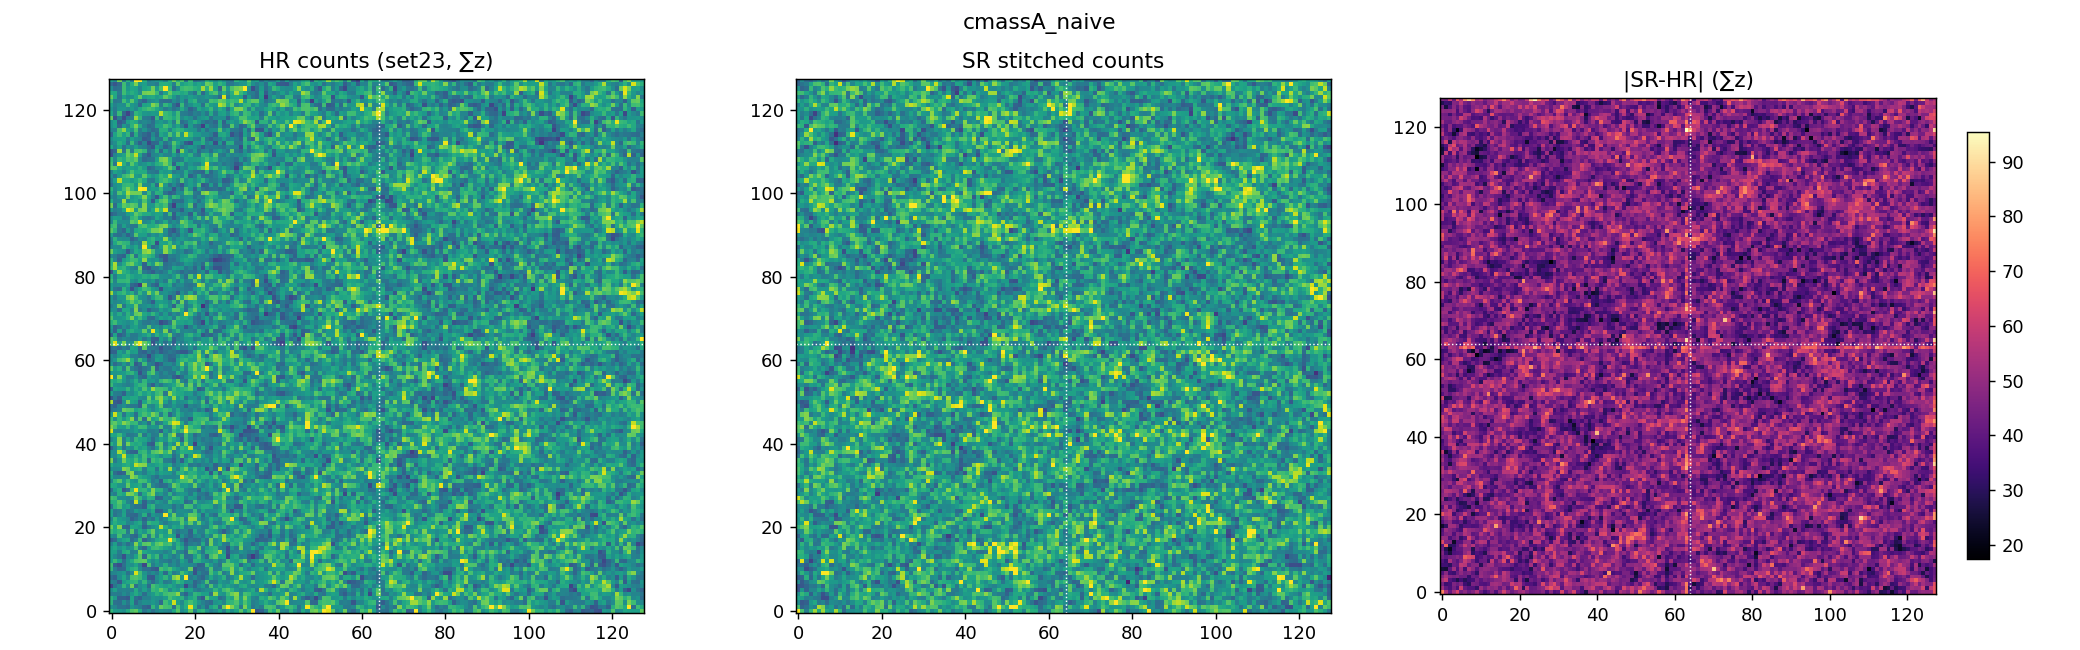
\includegraphics[width=0.95\linewidth]{figures_cmass/seam_cmassA_naive_slice.png}
\caption{Projected count maps for one test box (Arm A): HR, stitched SR, and the
absolute residual $|\mathrm{SR}-\mathrm{HR}|$. White dotted lines mark the
$x{=}64$, $y{=}64$ core boundaries; the residual shows no elevated ridge along
them.}
\label{fig:srs-seam}
\end{figure}

\paragraph{Per-scale diagnostic panels.} Figure~\ref{fig:srs-pkpanel} shows the
full-box $P(k)$, transfer, and cross-coherence for Arm A. The transfer sits near
$1$ at all scales (right amount of power); the cross-coherence is near $1$ at
large scales and falls toward small scales (structure placement is recovered at
large scales only). The per-patch panel
(\texttt{figures\_cmass/pk\_panel\_patch\_cmassAfix.png}) and the projection panels
(\texttt{projection\_box\_cmassAfix\_set23.png},
\texttt{projection\_patch\_cmassAfix\_set23\_p0.png}) tell the same story; Arm~B's
panels carry the \texttt{cmassB} suffix.

\begin{figure}[t]
\centering
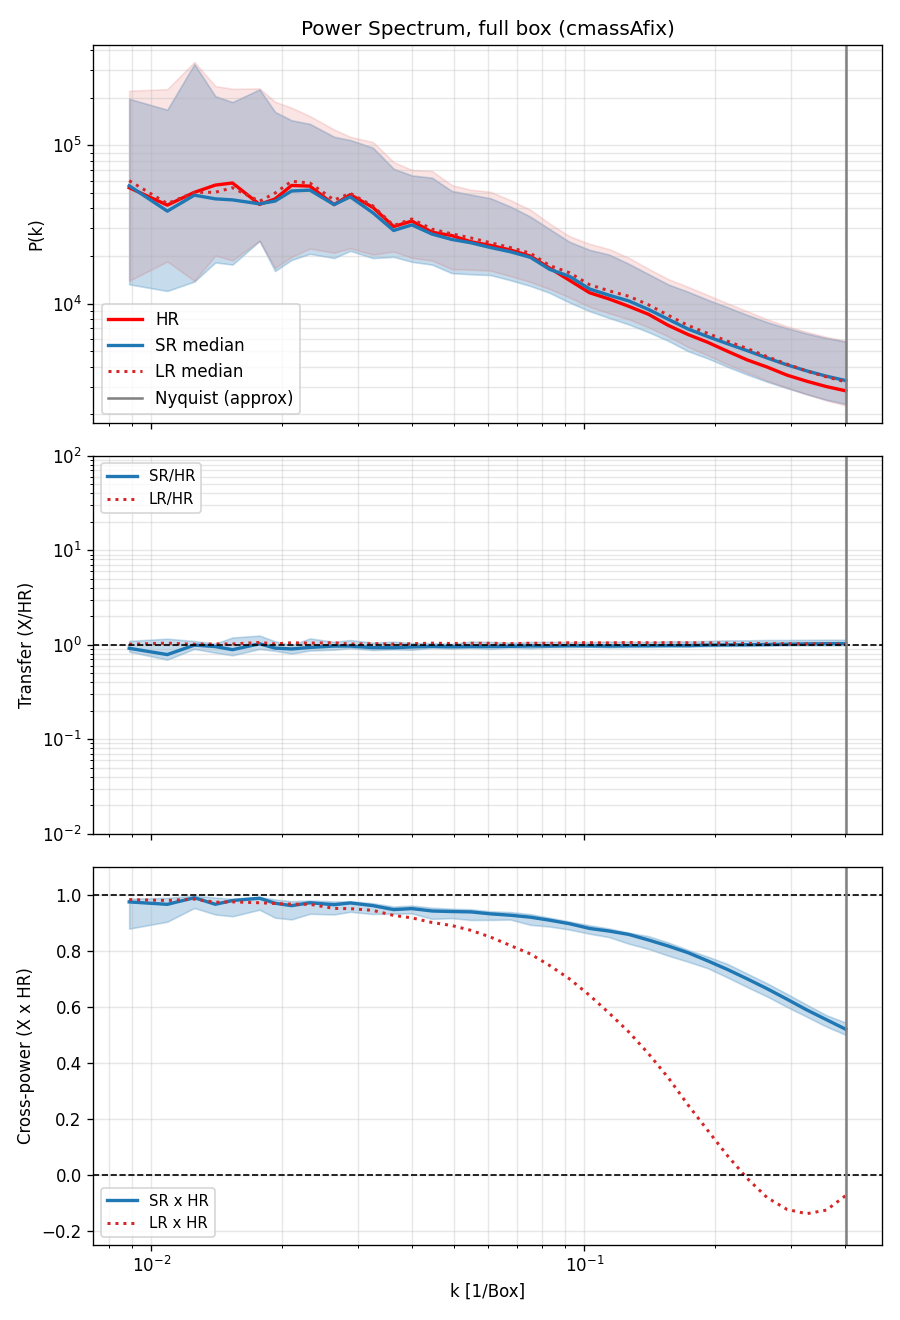
\includegraphics[width=0.5\linewidth]{figures_cmass/pk_panel_box_cmassAfix.png}
\caption{Full-box diagnostic for the conditioned generator (fiducial cosmology,
$16$ test boxes): $P(k)$ of HR (red), SR (blue median $+$ band), and LR (dotted
red); transfer $T(k)=P_X/P_\text{HR}$ on a linear axis with the 16 to 84
percentile band for both SR and LR, the legend reporting the RMS deviation of
each ratio from unity; and cross-coherence $r(k)$. The SR median transfer sits
below unity for $k<0.1$, a systematic large-scale power deficit of roughly 5 to
10 percent, while LR sits slightly above unity; SR does not tighten the transfer
scatter relative to LR. In $r(k)$, SR stays near unity to smaller scales while
LR decorrelates.}
\label{fig:srs-pkpanel}
\end{figure}

\subsection{Diagnostic: What is NOT Working}

\paragraph{Small-scale structure decorrelates, and this is fundamental.} SR
matches HR cell-by-cell at large scales ($r{=}0.95$ for $k<0.05$) but loses the
match at small scales ($r{=}0.40$ for $k>0.2$, Table~\ref{tab:srs-match}). This
is not a capacity bug: it is set by how much information the LR input carries
about HR. LR and HR share large-scale modes but the voxel-by-voxel LR$\leftrightarrow$HR
correlation is only $\approx0.06$, so the exact small-scale realization is simply
not present in the input. The model can match the small-scale \emph{statistics}
(transfer $\approx1$, real-space std ratio $1.008$) but cannot reproduce the
exact placement of individual halos. The noise injection
(Eq.~\ref{eq:srs-residual}) exists precisely because of this: it draws a
plausible small-scale field rather than regressing to a blur.

\paragraph{Per-box total-count scatter.} The total halo count is conserved on
average but with $\sim17\%$ per-box scatter ($\sum\mathrm{SR}/\sum\mathrm{HR}=
0.965\pm0.172$). A count-aware output head (predict a rate and sample Poisson
counts) would tighten this; it is the one clearly addressable imperfection. \SG{I would think this isn't necessary to fix, we don't care about the number of halos after all.}

\paragraph{Overlap suppresses small-scale power.} Arm B's overlap blending lowers
the small-scale transfer to $0.88$ (Table~\ref{tab:srs-pk}), so on the power
spectrum the naive Arm A is the better super-resolver. Overlap removes a small
generic boundary ripple but buys no fidelity, because on this continuous count
data there is no real seam to fix, the clean version of the mentor 2.1 vs 2.2
comparison.

\paragraph{Where the cosmology value is.} At the power spectrum level the raw LR
field is already close to HR, since they share large-scale modes, so the power
spectrum is a forgiving summary with little headroom. The model's value is at the
field level (variance, voids, small-scale structure), which the power spectrum
summary is insensitive to. The corrected cross-fidelity in
\S\ref{sec:srs-correction} bears this out: SR and LR are indistinguishable at the
power spectrum level, but at the field level an SR-trained posterior transfers to
HR while an LR-trained one does not.

\subsection{What I'm Trying Next}
\label{sec:srs-next}

The diagnostics above point to one limit that may be fundamental (small-scale
decorrelation) and a few that are clearly fixable (count scatter, small-scale
realism). The plan below is ordered so that we \emph{measure} the limit before
spending effort trying to beat it. None of these results are in yet; this is the
roadmap, not an experiment log.

\paragraph{Step 0, measure the information ceiling first.} Before trying to
improve the small-scale match, we need to know whether $r{=}0.40$ at small scales
(Table~\ref{tab:srs-match}) is the best any model could do from this input, or a
weakness of the current one. Two cheap diagnostics settle it:
\begin{itemize}
  \item \textbf{LR$\leftrightarrow$HR cross-coherence $r_\text{LR,HR}(k)$.} The
  cross-coherence of the \emph{raw input} against HR (no model) is the ceiling:
  no function of LR can place small-scale structure better than the input
  already correlates with HR. If $r_\text{SR,HR}(k)\approx r_\text{LR,HR}(k)$ at
  small $k$, the model is already at the ceiling and the limit is fundamental;
  if it sits well below, there is recoverable structure left on the table. (Only
  per-box $P(k)$ is currently saved, not the cross-spectrum, so this needs one
  re-run that keeps the fields.)
  \item \textbf{No-noise ablation.} Train the same generator with the noise
  injection off (a plain regressor). Theory predicts this should \emph{raise} the
  small-scale cross-coherence a little (a regressor targets the conditional mean,
  the best cell-by-cell predictor) but \emph{lower} the small-scale transfer well
  below $1$ (the conditional mean is blurry). Seeing exactly that trade-off would
  confirm that the noise/GAN is the right choice for a power-spectrum target, and
  would quantify how much cell-by-cell accuracy is being traded for correct
  statistics.
\end{itemize}

\paragraph{Step 1, fix the count scatter and small-scale realism (independent
of the ceiling).} These help regardless of what Step 0 finds:
\begin{itemize}
  \item \textbf{Count-aware (Poisson) output head.} Instead of predicting a
  count directly, predict a non-negative rate $\lambda$ per cell and sample the
  count as $n\sim\mathrm{Poisson}(\lambda)$. Halo counts are discrete and sparse,
  so a Poisson head models the small-scale graininess as actual shot noise rather
  than a smeared residual, and should tighten the $\sim17\%$ per-box total-count
  scatter (Table~\ref{tab:srs-match}), the one clearly addressable imperfection.
  \item \textbf{Explicit statistics terms in the loss.} Add a one-point PDF /
  variance matching term so small-scale sharpness is enforced directly, rather
  than relying on the adversarial term alone to find it.
  \item \textbf{Loss rebalance.} The current weights are $\lambda_\text{rec}{=}2$,
  $\lambda_\text{pk}{=}2$, $\lambda_\text{adv}{=}1$
  (Eq.~\ref{eq:srs-lossG}). The $L_1$ term blurs; lowering it and raising the
  adversarial weight should push toward correct statistics, at a known cost in
  cell-by-cell accuracy, per the same trade-off as the no-noise ablation.
\end{itemize}

\paragraph{Step 2, extract more of the available information (only if Step 0
shows headroom).} If $r_\text{SR,HR}$ sits below the LR$\leftrightarrow$HR
ceiling, the model is under-using its input. A larger receptive field, or feeding
each patch more neighbour context, would let it use more of the LR field to
predict the residual. This only helps if there is headroom to recover.

\paragraph{Step 3, raise the ceiling by changing the \emph{input}, not the
model.} The small-scale cell-by-cell limit is set by the information in the LR
input (the voxel-by-voxel LR$\leftrightarrow$HR correlation is only
$\approx0.06$). No amount of model capacity raises that; only more informative
inputs do. Candidates: feed the shared small-scale \emph{initial conditions}
(which the coarse LR count field has discarded), or add the LR velocity / particle
fields. This is the only route to a meaningful gain in small-scale cross-coherence,
and is the natural bridge to the displacement-field model of \S5, which already
carries that extra information.

\paragraph{Summary.} Steps 0--1 are the near-term plan: measure the ceiling, then
add a Poisson head and statistics losses to fix the count scatter and sharpen the
small-scale field. Steps 2--3 are contingent on what Step 0 reveals. For a
cosmology deliverable the priority is statistical fidelity (which Steps 0--1
target); exact small-scale reconstruction (Step 3) is a larger, input-level
change worth it only if cell-by-cell recovery becomes the goal.

\subsection{Follow-Up Results: New Protocol from the Mentor Meeting}
\label{sec:srs-followup}

A mentor meeting after the report above changed two things about how we train
and evaluate this model. First, the real goal is not to match HR with SR by
itself. The real goal is to train a posterior model on SR output and have it
work well when it is tested on real HR data, since HR simulations are too
expensive to train a posterior model on directly. Second, the power spectrum
term was removed from the training loss, since it was also our main success
metric and that is a weak test. This subsection reports what we found. Some of
the training runs below are still in progress at the time of writing, so
numbers marked as current are read from the latest completed epoch, not a
final result.

\paragraph{Held-out check: the bispectrum.} A fair worry is that our power
spectrum result looks good only because the power spectrum was also in the
training loss. To check this we measured the bispectrum, a higher-order
statistic that was never used anywhere in training or model selection. If SR
only matches the power spectrum and nothing else, the bispectrum should show
no improvement over the raw LR input.

\begin{figure}[t]
\centering
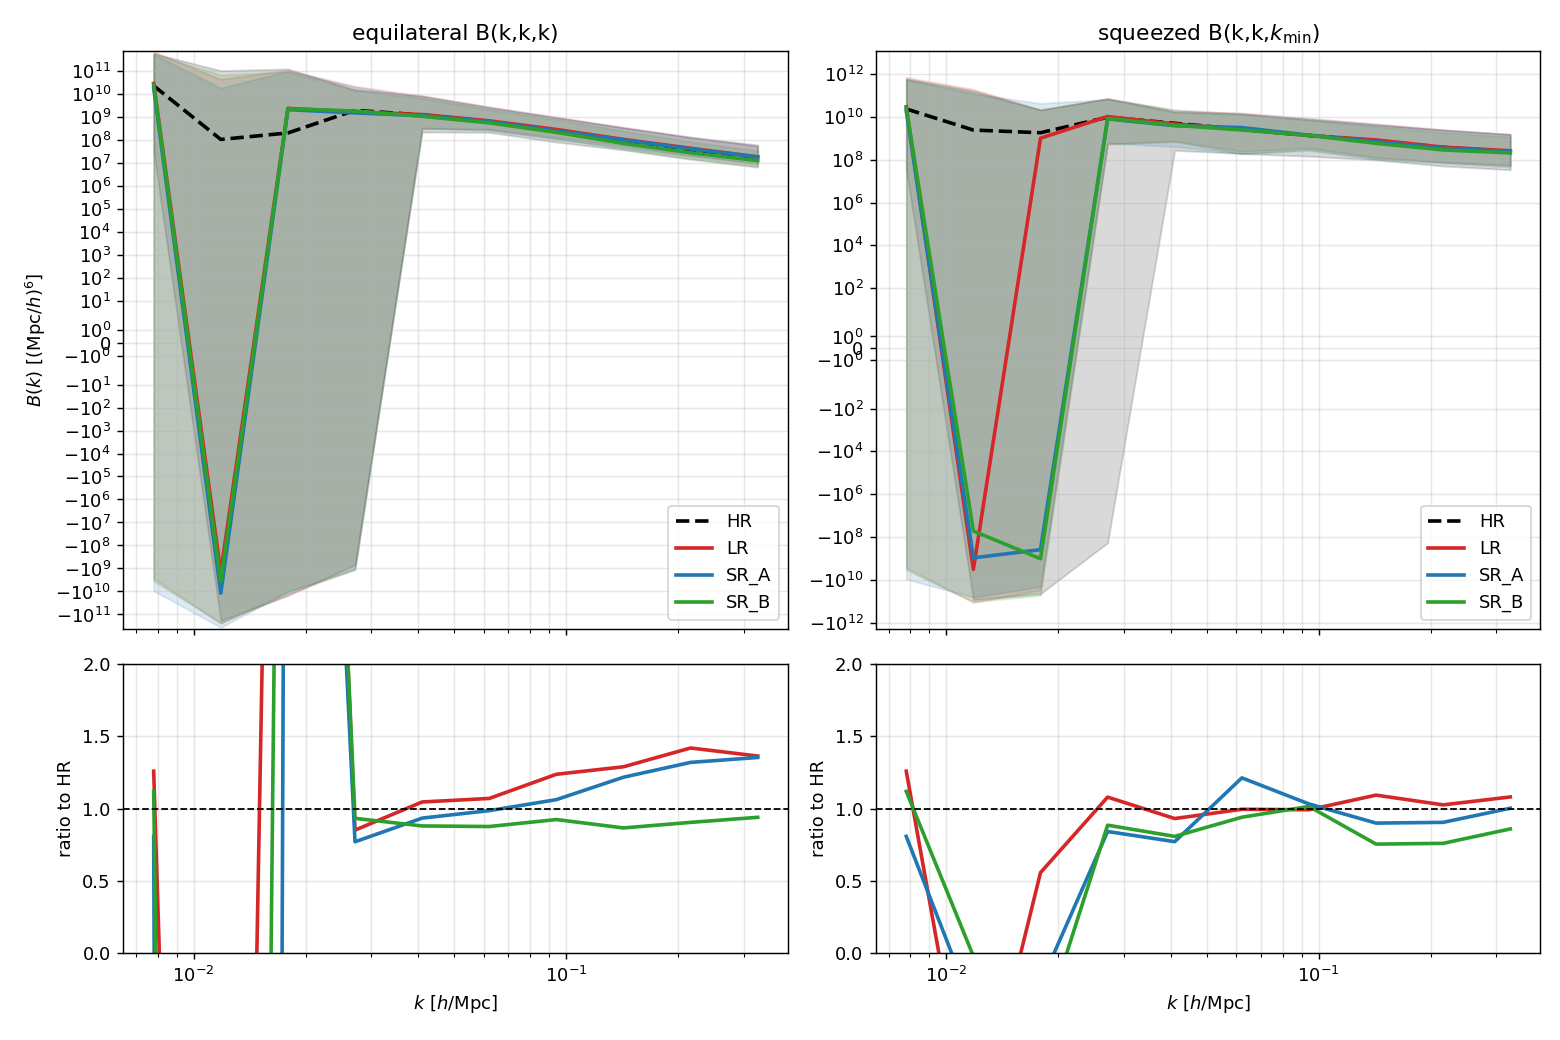
\includegraphics[width=0.95\linewidth]{figures_cmass/bispectrum_hr_lr_srA_srB.png}
\caption{Bispectrum of HR, LR, and SR (both arms), on $16$ test boxes. Top:
equilateral and squeezed bispectrum, HR in black. Bottom: ratio to HR. SR
removes most of the systematic excess that LR has at the plotted scales,
without ever training on this statistic.}
\label{fig:srs-bispec}
\end{figure}

On the equilateral configuration, LR sits about $6$ to $13$ percent above HR
across the middle range of scales. SR removes most of this gap without ever
seeing a bispectrum during training, and it does this for both arms. This is
evidence that the model is not simply fitting the training metric. It is
correcting real structure in the field that also shows up in a statistic it
never saw. (The figure uses the earlier models trained \emph{with} the power
spectrum loss; the no-Pk models of the following paragraphs preserve the
bispectrum at least as well, so removing that loss did not degrade this
held-out statistic either.)

\paragraph{Removing the power spectrum loss.} Following the meeting, we
retrained the model with the power spectrum term switched off
($\lambda_\text{pk}{=}0$ in Eq.~\ref{eq:srs-lossG}), so the loss is only the
adversarial and $L_1$ terms. We also changed which checkpoint counts as "best"
to the real-space $L_1$ error, since selecting on the power spectrum would
have been the same kind of leak we were trying to remove.

\begin{figure}[t]
\centering
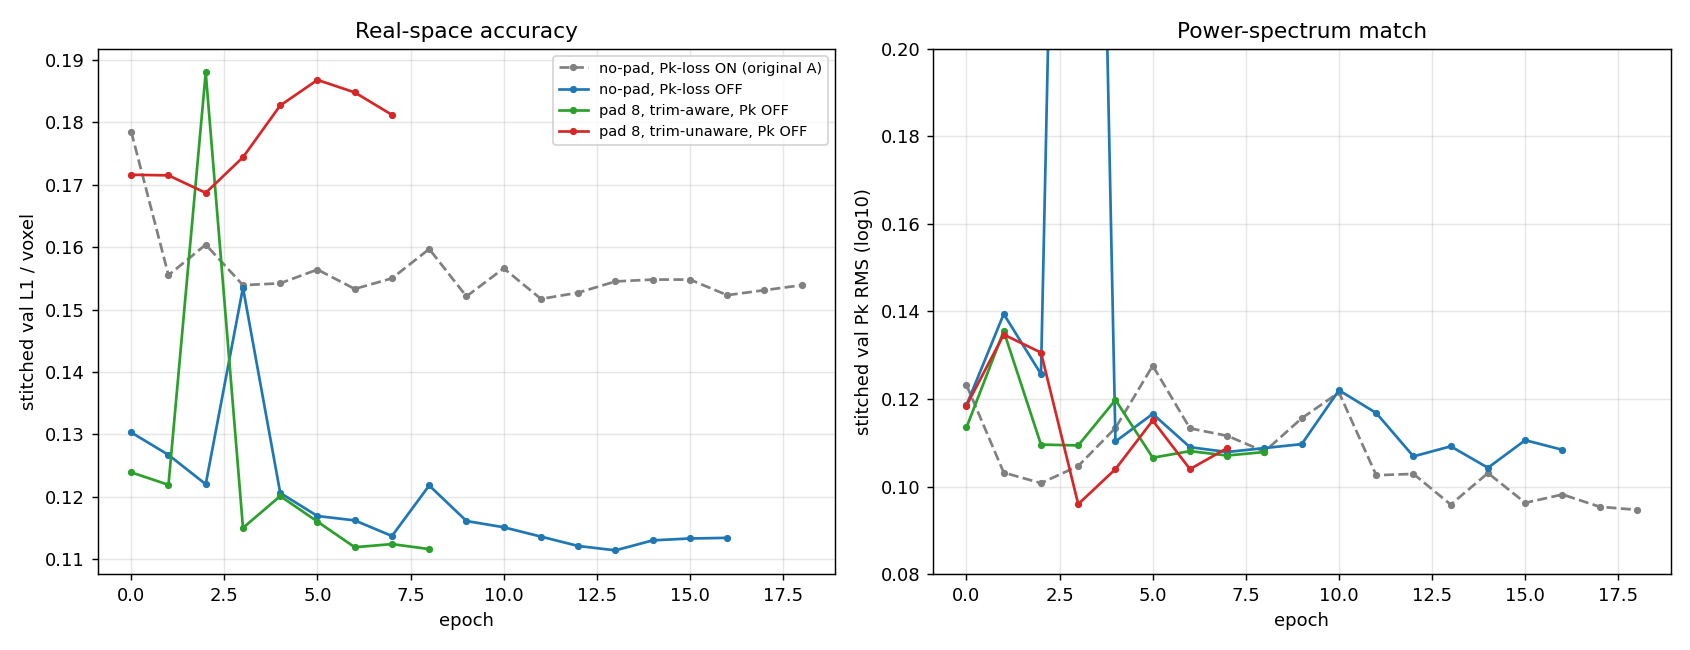
\includegraphics[width=0.98\linewidth]{figures_cmass/protocolv2_cmass.png}
\caption{Stitched validation curves under the new protocol (power spectrum
loss off). Left: real-space $L_1$ error. Right: power spectrum RMS error. Grey
dashed: the original Arm A with the power spectrum loss on, for comparison.
These runs are still training; curves stop at the most recent completed
epoch.}
\label{fig:srs-protocolv2}
\end{figure}

Two things stand out so far. First, without the power spectrum term, the
real-space $L_1$ error becomes clearly better than the original run at the
same point in training (left panel, blue and green curves sit below the grey
dashed curve). Second, the power spectrum error does get a little worse
without its loss term, but it does not collapse: it settles into roughly the
same range as before, just a bit noisier. So the power spectrum term was
buying us a small amount of power spectrum accuracy at a real cost in
real-space accuracy. It was not the only reason the power spectrum matched
well; the adversarial and reconstruction terms carry most of that on their
own.

\paragraph{Does padding help, once the power spectrum loss is out of the way?}
The report above found that padding (Arm B) did not beat no padding (Arm A) on
the power spectrum. The mentor pointed out two different ways this could
happen, and that they make different, testable predictions:
\begin{itemize}
  \item \textbf{Trim-aware.} The model is trained knowing that only the middle
  part of its output will be kept; the loss only looks at that middle part.
  This is what Arm B already did. If this is working correctly, padding should
  train at least as well as no padding, since it has strictly more context for
  the same target.
  \item \textbf{Trim-unaware.} The model is trained as if its whole padded
  output matters, including the edge region that gets thrown away later. If
  the model leans on that edge region during training, it should look fine
  during training but generalize worse once the edge is cut off at test time.
\end{itemize}
We trained both versions with the power spectrum loss off, so the comparison
is not confused by that term. Figure~\ref{fig:srs-protocolv2} shows all three
runs together (no padding, trim-aware padding, trim-unaware padding).

The trim-aware version (green) matches or beats no-padding (blue) on both
real-space error and power spectrum error at almost every epoch measured so
far. This supports the first prediction: once the model is told correctly what
part of its output is graded, more context helps rather than hurts. The
trim-unaware version (red) is clearly worse on real-space error than both
other runs, and does not close that gap as training continues. This supports
the second prediction: a model that is allowed to rely on the part of its
output that gets discarded at test time pays for that at test time. Put
together, the original result that padding did not help was most likely
caused by the power spectrum loss, not by padding itself.

We also reran the older, padding-with-power-spectrum-loss model for more
epochs to check whether it had simply not been trained long enough. Fifteen
additional epochs did not beat its early best score, so that run was not
undertrained; the training recipe, not the training time, was the limiting
factor.

\subsection{The Goal Metric: Corrected Cross-Fidelity Results}
\label{sec:srs-correction}

\paragraph{The bug.} After the analysis above, a routine physical sanity check
failed in a way that could not be real: the amplitude of the power spectrum had
essentially zero correlation with $\sigma_8$, and a fit of the power spectrum to
the five parameters explained only $0.2\%$ of the variance. The power spectrum
amplitude must scale with $\sigma_8$, so this pointed to a labeling error, not to
physics. Tracing it, we found that the processed count fields were written in
string-sorted simulation order ($0, 1, 10, 100, 1000, \dots$) while the cosmology
table is indexed numerically. Field number $k$ is therefore the halo field of
simulation string-sort$(k)$, not simulation $k$, so every field in the whole
pipeline was paired with the wrong cosmology. We proved this exactly: using the
original halo catalogs, the field halo count matches the catalog count under the
string-sort permutation for all $2000$ simulations, while the identity mapping
matches only the two fixed points. We corrected the cosmology table to field
order, backed up the old one, and patched the builder so it cannot regenerate the
wrong order.

\begin{figure}[h]
\centering
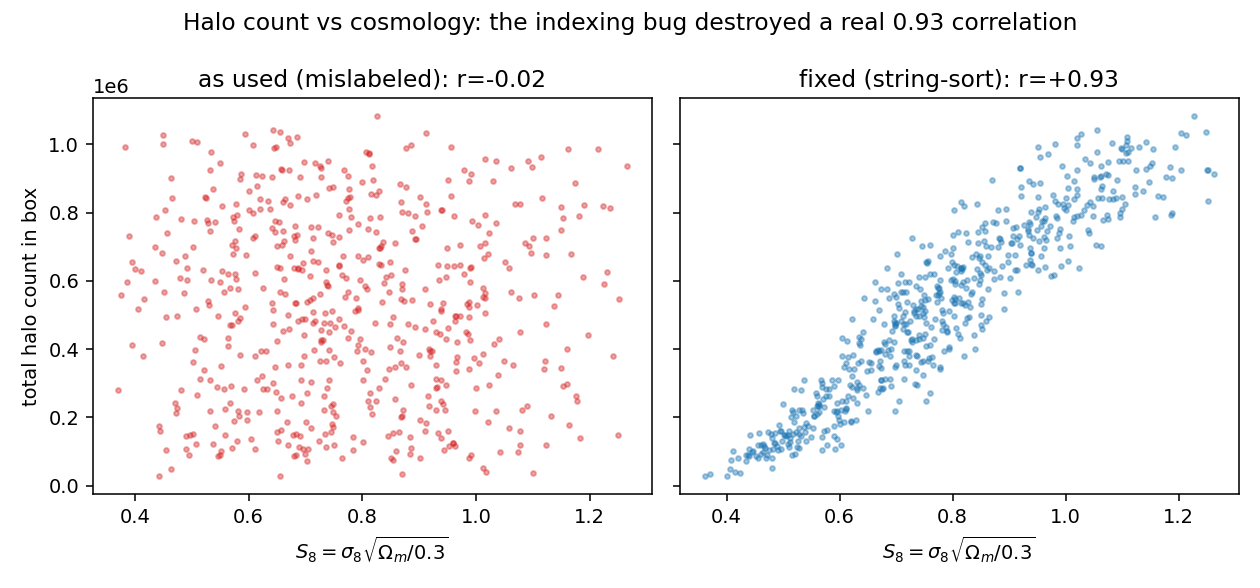
\includegraphics[width=0.85\linewidth]{figures_cmass/labelbug_count_vs_s8.png}
\caption{The indexing bug in one picture. Total halo count in a box against
$S_8 = \sigma_8\sqrt{\Omega_m/0.3}$. As the pipeline used the labels (left) the
correlation is zero; with the string-sort mapping corrected (right) the true
$0.93$ correlation reappears. Halo abundance must track $S_8$, so the left panel
was the signature of a labeling error, not of uninformative data.}
\label{fig:srs-labelbug}
\end{figure}

\paragraph{What this changes, and what it does not.} Every cosmology number we
computed before this point used the labels and is affected; the earlier
cross-fidelity tables have been removed and are replaced by the corrected results
below, and the earlier reading that the SR-versus-LR difference was an irreducible
coin flip was itself a product of the mislabeling. The results that do not use the
labels are unaffected and still stand: the power spectrum match of SR to HR, the
held-out bispectrum, the field-match statistics, the seam test, and the real space
error. The generator conditions on the cosmology as a style vector and was trained
with the scrambled labels, so its conditioning was uninformative during training;
we return to this at the end.

\paragraph{The data is informative after all.} With correct labels the picture
inverts. A halo count in this suite carries a strong cosmological signal: the
total halo count alone correlates with the combination $S_8 = \sigma_8
\sqrt{\Omega_m/0.3}$ at $0.93$ and with $\Omega_m$ at $0.85$. A Fisher forecast on
a single-box power spectrum now explains $98\%$ of the variance, where it
explained $0.2\%$ before, and it constrains $\Omega_m$ and $\sigma_8$ well, with
$\Omega_b$, $h$ and $n_s$ weak or unconstrained, which is the textbook pattern for
a low-redshift halo field. The field-level network tells the same story: after the
fix its predicted $\Omega_m$ correlates with the truth at $0.90$ on both training
and test boxes, where before the fix the correlation was zero and the output was a
constant. So the earlier conclusion that a single box carries almost no cosmology
was an artifact of the labeling, not a property of the data.

\begin{figure}[h]
\centering
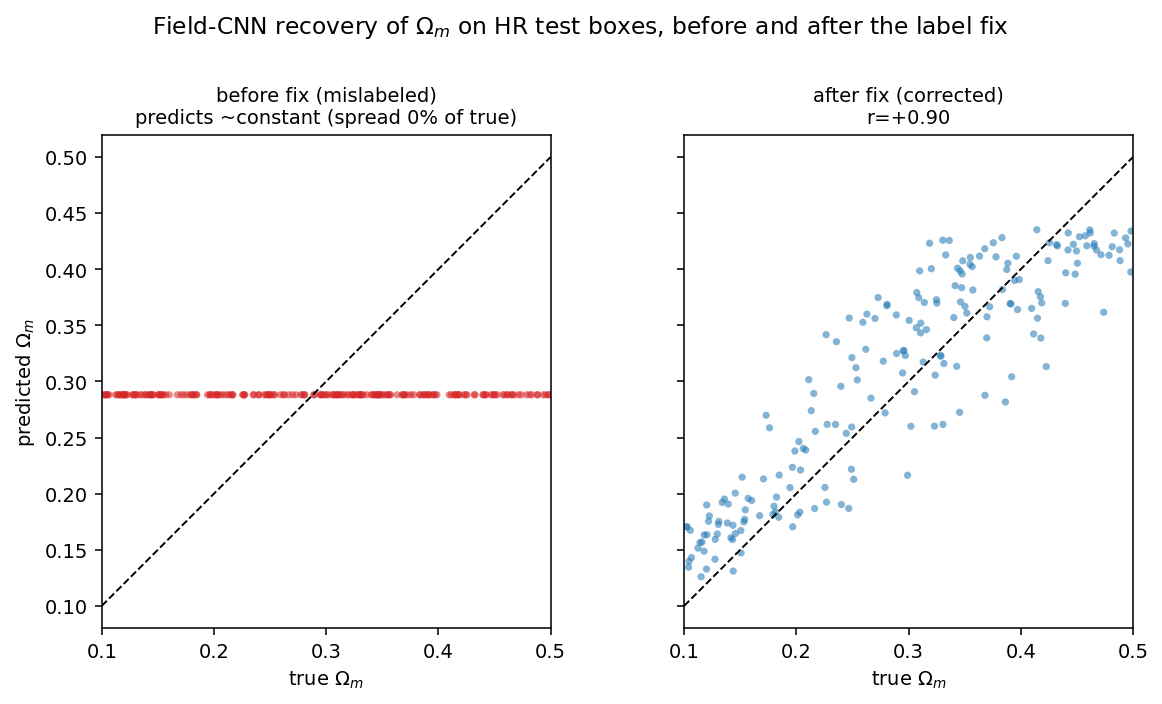
\includegraphics[width=0.82\linewidth]{figures_cmass/field_recovery_Om_cmass.png}
\caption{Field-level CNN recovery of $\Omega_m$ on HR test boxes, before and after
the label fix. Before (left) the prediction is flat and uncorrelated with the
truth (the network returns a near-constant); after (right) it tracks the diagonal
at a correlation of about $0.90$, on both training and test boxes. Same
architecture, same data, only the labels changed.}
\label{fig:srs-recovery}
\end{figure}

\begin{figure}[h]
\centering
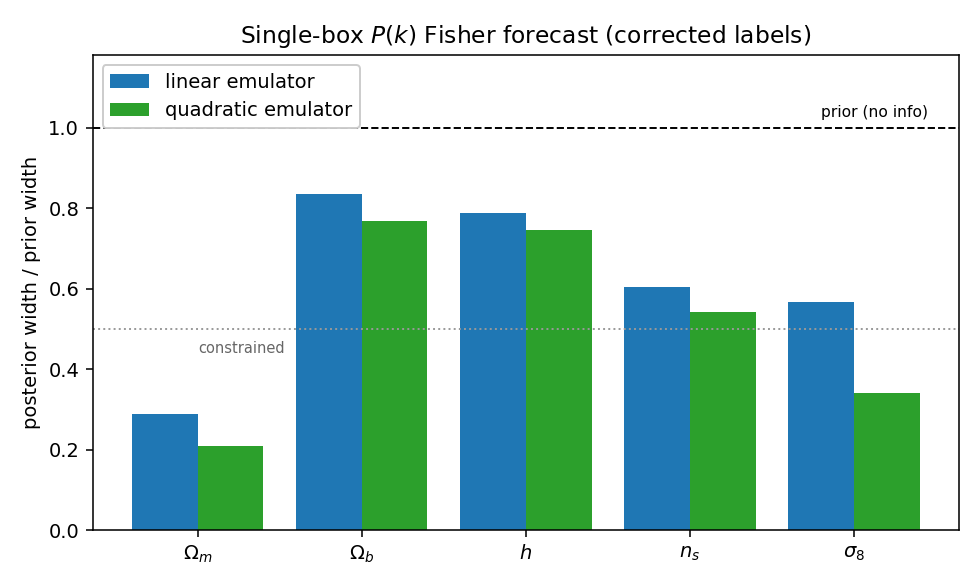
\includegraphics[width=0.72\linewidth]{figures_cmass/fisher_corrected_cmass.png}
\caption{Fisher forecast for a single-box power spectrum with corrected labels:
posterior width divided by prior width per parameter (lower means better
constrained, $1$ means no information). $\Omega_m$ is well constrained and
$\sigma_8$ is constrained, while $\Omega_b$, $h$ and $n_s$ are weak, the textbook
pattern for a low-redshift halo field. Two emulators (linear average slope and
quadratic at the prior centre) bracket the estimate.}
\label{fig:srs-fisher}
\end{figure}

\paragraph{Corrected cross-fidelity, and where SR helps.} We re-ran the goal
metric with correct labels at two levels, the power spectrum summary and the full
field. We train the posterior on one source, apply it to HR, and compare to a
posterior trained on HR, using an ensemble of independently retrained estimators
so the numbers are not single draws. Table~\ref{tab:srs-corrected} gives the
result.
\begin{table}[h]
\centering
\caption{Corrected cross-fidelity KL to HR (posterior trained on the named source,
evaluated on HR), lower is better, with the HR-to-HR floor for reference. Summary
uses the power spectrum; field uses a three-dimensional CNN posterior on the full
box.}
\label{tab:srs-corrected}
\begin{tabular}{lccc}
\toprule
level & LR (raw) & SR & HR floor \\
\midrule
summary $P(k)$ & $0.032$ & $0.088$ & $0.028$ \\
field (CNN)    & $0.49 \pm 0.81$ & $\mathbf{0.024}$ & $0.022$ \\
\bottomrule
\end{tabular}
\end{table}
\begin{figure}[h]
\centering
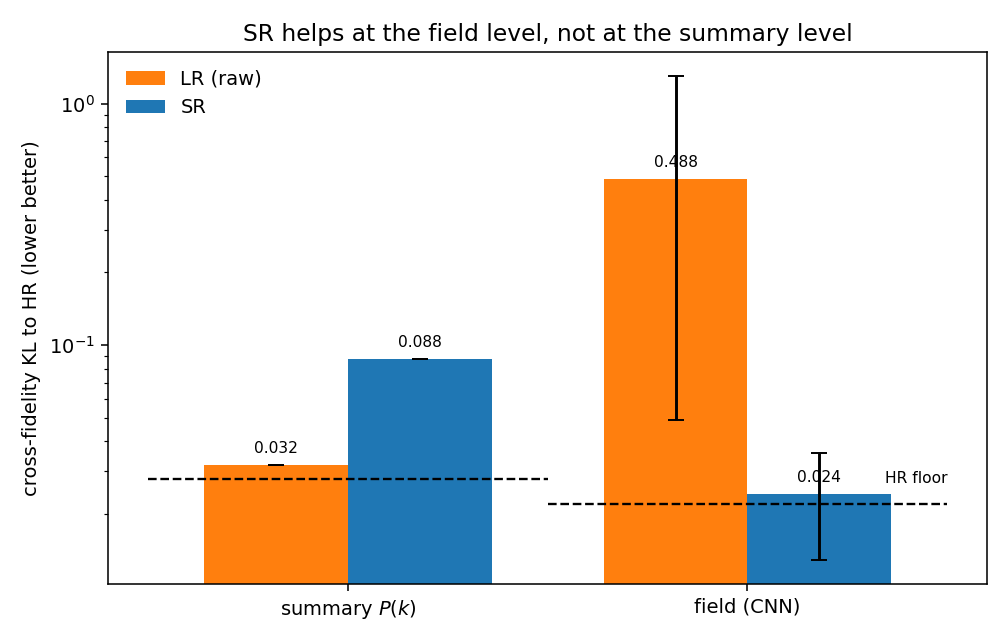
\includegraphics[width=0.7\linewidth]{figures_cmass/crossfid_corrected_cmass.png}
\caption{Corrected cross-fidelity KL to HR (log scale, lower is better) at the two
levels, with the HR-to-HR floor shown as the dashed line. At the summary level the
raw LR field is already at the floor and SR does not help. At the field level, an
LR-trained posterior does not transfer to HR (large and unstable), while an
SR-trained posterior sits at the floor. SR helps exactly where it corrects the
field.}
\label{fig:srs-crossfid-corrected}
\end{figure}
The two levels point in opposite directions, and both make sense. At the summary
level the raw LR power spectrum is already at the HR floor, so an LR-trained
posterior transfers to HR as well as an HR-trained one does, and there is no gap
for SR to close; SR even hurts a little, because the generator reshapes the
small-scale power in a way that does not match how HR responds to cosmology. At
the field level the raw LR box looks different enough from HR that an LR-trained
posterior does not transfer, and it does so unreliably, sometimes acceptably and
sometimes catastrophically, which is why its number carries such a large spread.
SR corrects the field to look like HR, so an SR-trained posterior transfers to HR
reliably, at the floor. This is exactly the deployment case the project is built
on, train the inference model on cheap SR-corrected boxes and apply it to
expensive HR, and at the field level SR makes it work where raw LR does not.

\paragraph{Padding on the goal metric.} We ran the two padding variants through
the corrected cross-fidelity at the summary level as well
(Table~\ref{tab:srs-padding}). Among the SR models the ordering from the earlier
report survives: no padding is best on the goal metric, trim-aware padding is
worse, and trim-unaware is worst, so for the cosmology objective the no-padding
model is the one to use. All three sit above the raw LR control at this level,
consistent with LR already being HR-like on the power spectrum. One number does
change under the fix: the mislabeled data made trim-unaware look catastrophic (a
factor of several hundred above the others), while with correct labels it is the
weakest variant by about a factor of two, not a blow-up. Its real-space error
(Figure~\ref{fig:srs-protocolv2}) remains the clearest and most direct sign that
it is the least reliable model.
\begin{table}[h]
\centering
\caption{Corrected cross-fidelity KL to HR at the summary (power spectrum) level
for the SR padding variants, with the LR control and the HR floor. Lower is
better. Field-level padding numbers are future work.}
\label{tab:srs-padding}
\begin{tabular}{lc}
\toprule
model & summary cross-fidelity KL \\
\midrule
SR, no padding & $\mathbf{0.087}$ \\
SR, trim-aware padding & $0.127$ \\
SR, trim-unaware padding & $0.172$ \\
\midrule
LR (control) & $0.031$ \\
HR floor & $0.028$ \\
\bottomrule
\end{tabular}
\end{table}

\paragraph{Bottom line.} With the labels fixed, the cosmology question has a
clear answer. The data constrains $\Omega_m$ and $\sigma_8$ from a single box. At
the power spectrum level the raw LR field is already HR-like, so SR is not needed
there and slightly hurts. At the field level, which is what SR actually corrects,
an SR-trained posterior transfers to HR at the floor while a raw LR one does not,
so SR provides a real and reliable cosmology benefit exactly where it operates.
Trim-unaware padding is still the weakest variant, worst on the goal metric and
on real-space error, though the label fix shrinks its apparent failure from
catastrophic to about a factor of two. Two honest caveats remain: the
field-level LR number has a wide spread and rests on a handful of retrained
networks, so the size of the gap should be firmed up with more seeds; and because
the generator was trained with the scrambled labels, its cosmology conditioning
was uninformative, so a retrain with correct conditioning may sharpen the SR
result further. Neither caveat changes the direction: with correct labels, SR
helps cosmology at the field level.

\paragraph{A data reliability note.} Partway through these runs, the shared
data storage this project reads from filled up completely, which caused a few
training jobs to fail with a file briefly appearing missing even though it was
not actually deleted. We added a retry step to the data loader and resumed
each affected run from its last saved checkpoint, so no real training progress
was lost. This is a shared infrastructure issue, not a problem with the data or
the method.

\subsection{Files}
\begin{itemize}\itemsep0pt
  \item Data and patching: \texttt{data/patch\_dataset\_cmass.py}
  (shared ops in \texttt{data/patch\_dataset\_real.py})
  \item Model: \texttt{map2map/models/styled\_srsgan.py}
  (\texttt{G\_correct}, \texttt{D\_const})
  \item Training: \texttt{train\_patch\_cmass.py};
  run script \texttt{scripts/train\_patch\_cmass.slurm}
  \item Inference and stitching: \texttt{infer\_stitch\_cmass.py}
  \item Seam eval: \texttt{analysis/eval\_seam\_cmass.py}
  \item Box / per-patch diagnostics: \texttt{analysis/diag\_cmass.py}
  \item SR-vs-HR match stats: \texttt{analysis/match\_stats\_cmass.py}
  \item SR-vs-HR power-spectrum figure: \texttt{analysis/plot\_sr\_vs\_hr.py}
  \item Bispectrum (held-out statistic): \texttt{analysis/bispectrum\_cmass.py}
  \item Training loss curves: \texttt{analysis/plot\_losses\_cmass.py}
  \item Cross-fidelity posterior evaluation: \texttt{evaluate.py} (SR-trained
  or LR-trained posterior evaluated on HR $P(k)$)
  \item Protocol-v2 (no-Pk-loss, padding-variant) training curves:
  \texttt{analysis/plot\_protocolv2\_cmass.py}
  \item Power spectrum on counts: \texttt{analysis/power\_spectrum.py}
  (estimator \texttt{counts}); differentiable training version
  \texttt{analysis/pk\_torch.py}
  \item Posterior and KL: \texttt{inference/nde.py}, \texttt{evaluate.py};
  end-to-end eval \texttt{scripts/eval\_cmass\_wrapper.slurm}
  \item Field-level posterior (three-dimensional CNN, moment-network loss):
  \texttt{models/field\_cnn.py}, \texttt{train\_field\_cnn.py};
  SR field generation \texttt{gen\_sr\_fields.py}; capacity and recovery
  diagnostics \texttt{overfit\_test.py}, \texttt{field\_diag.py}
  \item Outputs: \texttt{runs/patch\_cmass/}; figures: \texttt{figures\_cmass/}
\end{itemize}
 from main.tex, or paste inline.
% Figures referenced live in figures_cmass/ (set \graphicspath or copy them
% next to main.tex). Every number is from runs/patch_cmass/ and FINAL.md.
% =====================================================================

\section{SRS-styled-map2map-galaxy}
\label{sec:srs}

This section documents the second model in this work at the same level of
detail as \S5. Where \S5 corrects a Lagrangian \emph{displacement} field with a
point--voxel flow matcher, this model corrects an Eulerian \emph{halo count}
field with a styled GAN. The two share the same high-level goal, make a cheap
low-fidelity (LF) simulation look like an expensive high-fidelity (HF) one, 
but operate on different data and use a different architecture.

\paragraph{Goal.} Running an accurate (high-resolution) N-body simulation is
expensive; running a fast approximate one is cheap. We want a model that takes
\emph{only} the cheap LF field and produces a corrected field (we call it the
super-resolved or \textbf{SR} field) that matches the expensive HF field. At
inference the model never sees HF: the HF field is used only to train the model
and to grade it. So every result in this section answers one question: \emph{how
close is the SR field, built from LF alone, to the HF field it never saw?}

\paragraph{Terminology.} We work one cubic sub-volume at a time. We call the
$64^3$ output sub-volume a \textbf{core}, and the (possibly larger) input
sub-volume that the model reads a \textbf{patch}. When \texttt{pad}${=}0$ the
patch and the core coincide. We use \textbf{LR}/\textbf{LF} and
\textbf{HR}/\textbf{HF} interchangeably; the data here is named LR (input) and
HR (target).

\paragraph{Two arms.} We test the boundary treatment with two arms that are
identical except for one number:
\begin{itemize}
  \item \textbf{Arm A (naive, mentor 2.1):} \texttt{pad}${=}0$. Each $64^3$ core
  is corrected and placed edge-to-edge.
  \item \textbf{Arm B (overlap, mentor 2.2):} \texttt{pad}${=}8$. Each patch is
  grown to $80^3$ with real neighbour cells (periodic wrap), only the central
  $64^3$ core is kept and placed.
\end{itemize}

\subsection{Data Preprocessing}
\textit{Source: \texttt{cmass-ili}; loader \texttt{data/patch\_dataset\_cmass.py}.}

\paragraph{Input.} We have $2000$ paired simulations at redshift $z=0.5$, run
from shared initial conditions. Each pair is a low-fidelity field (LR, from the
FastPM particle-mesh code) and a high-fidelity field (HR, from a Quijote N-body
run). Both are stored as integer \textbf{halo count grids} of shape
$128\times128\times128$ on a periodic box of side $L_\text{box}=1000\
\mathrm{Mpc}/h$ (cell size $\approx 7.81\ \mathrm{Mpc}/h$). A cell value is the
number of halos whose position falls in that cell. The fields are sparse: most
cells are zero and the mean count per cell is small (the code caches one global
count scale, the mean HR count per cell measured over $50$ training sims).
Because LR and HR share initial conditions, they describe the same structure at
two fidelities. The correspondence is between the two halo catalogs \emph{as a
whole}: there is no known one-to-one matching between individual LR and HR
halos, only between the count fields they produce.

\paragraph{Cosmology labels.} Each simulation carries a style vector
$\mathbf s=(\Omega_m,\Omega_b,h,n_s,\sigma_8)\in\mathbb R^5$, parsed from that
sim's \texttt{config.yaml}.

\paragraph{Splits.} The on-disk lists give $1600$ train, $200$ validation, and
$200$ test simulations, split by simulation index.

\begin{figure}[t]
\centering
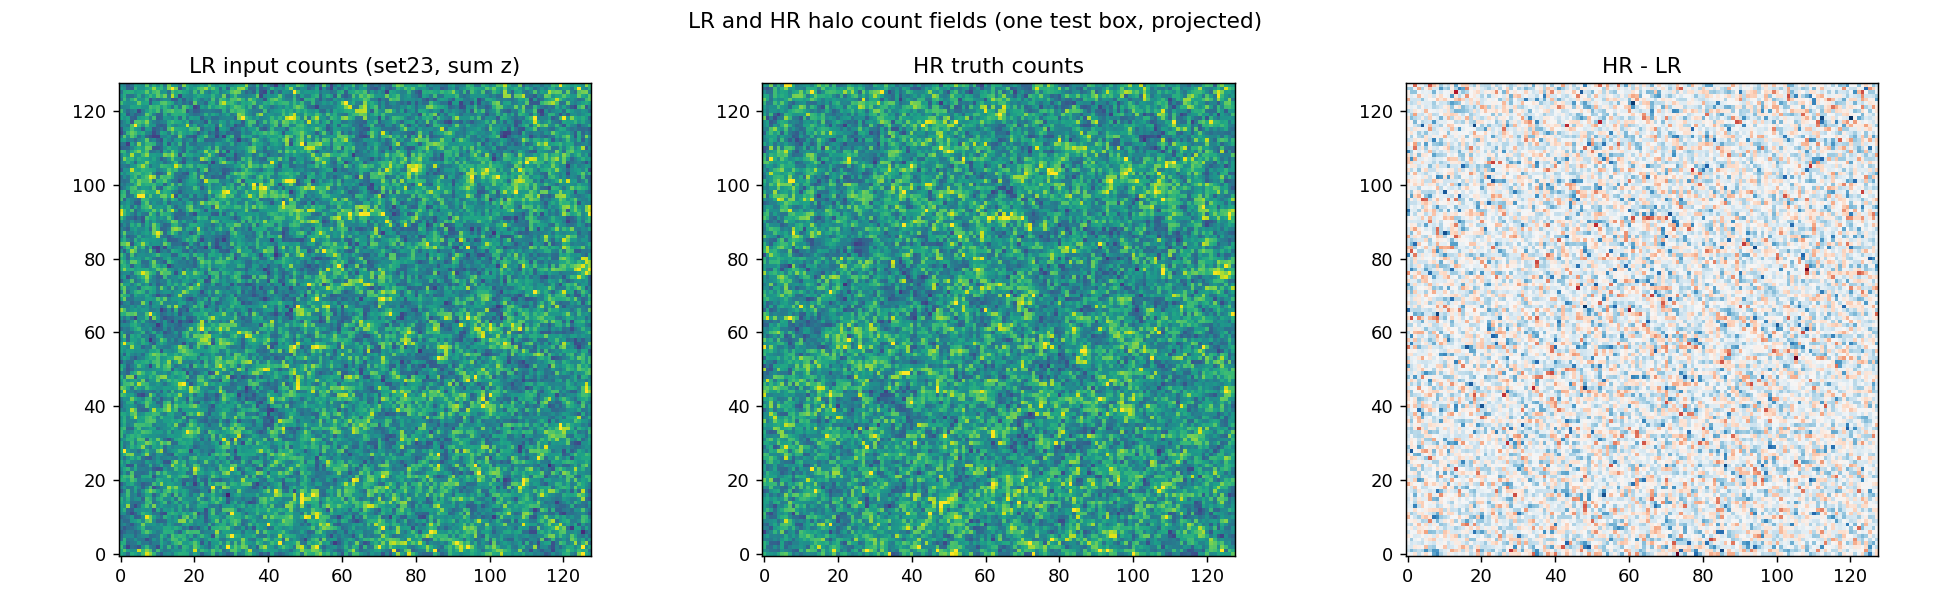
\includegraphics[width=0.9\linewidth]{figures_cmass/data_pair.png}
\caption{One LR/HR pair (projected count map). LR (FastPM, input) and HR
(Quijote N-body, target) share initial conditions and so share large-scale
structure, but differ cell-by-cell.}
\label{fig:srs-datapair}
\end{figure}

\paragraph{Model space (count transform).} The network does not learn on raw
counts; it learns in a compressed ``model space''. The default transform is
$\log(1+n)$, which tames the sparse heavy tail:
\begin{equation}
  y = \log(1+n), \qquad n = \exp(y)-1 \ \ (\text{clamped to } n\ge 0).
  \label{eq:srs-transform}
\end{equation}
Two alternative transforms exist in the code (\texttt{scale}: $n/\text{scale}$;
\texttt{delta}: model space is the overdensity itself), but all reported runs use
$\log(1+n)$. Power spectra are \emph{never} computed in model space; they are
always computed on the physical-count overdensity \SG{Is it okay if this is -1 when there are 0 halos?}
\begin{equation}
  \delta = \frac{n}{\bar n} - 1,
  \label{eq:srs-delta}
\end{equation}
with $\bar n$ the per-box mean count (the \texttt{perbox} setting used in all
runs).

\subsection{Data Pipeline (patching)}
\textit{Located in: \texttt{data/patch\_dataset\_cmass.py},
\texttt{data/patch\_dataset\_real.py} (shared patch ops).}

A model never sees the whole $128^3$ box at once. We cut the box into a
$2\times2\times2$ grid of $64^3$ \textbf{cores} (Table~\ref{tab:srs-notation}).
The cores tile the box exactly (stride $64$), so they reconstruct the box
bit-for-bit with no gaps and no double counting, the dataset's self-test
asserts this. Each model \emph{input} is a core grown by \texttt{pad} voxels on
every side, taken from the true neighbour cells with periodic wrap at the box
edge (\texttt{extract\_patch} uses \texttt{numpy.take(\dots, mode="wrap")}). So
with \texttt{pad}${=}8$ the input is $80^3$ and neighbouring patches overlap by
$2\cdot\texttt{pad}=16$ voxels; the HR \emph{target} is always the bare $64^3$
core. Because each simulation is one continuous periodic box that we crop
ourselves, the patches are real neighbours by construction, there is no data
seam (unlike the Lagrangian patches of \S5). \SG{Isn't the patch construction same in both?}

\begin{table}[t]
\centering
\caption{Notation for the CMASS count-field pipeline.}
\label{tab:srs-notation}
\begin{tabular}{llp{7.2cm}}
\toprule
Symbol & Value & Meaning \\
\midrule
$N_\text{full}$    & $128$ & full box side (voxels) \\
$P$ (\texttt{PATCH}) & $64$ & core side (voxels) \\
$N_\text{patches}$ & $8$ & cores per box ($2{\times}2{\times}2$) \\
\texttt{pad}       & $0$ (Arm A) / $8$ (Arm B) & halo width added to each face by periodic wrap \\
$L_\text{box}$     & $1000\ \mathrm{Mpc}/h$ & box side \\
$\mathbf s$        & $\in\mathbb R^5$ & cosmology vector $(\Omega_m,\Omega_b,h,n_s,\sigma_8)$ \\
$\bar n$           & per-box mean & mean count used to form $\delta=n/\bar n-1$ \\
\bottomrule
\end{tabular}
\end{table}

\begin{figure}[t]
\centering
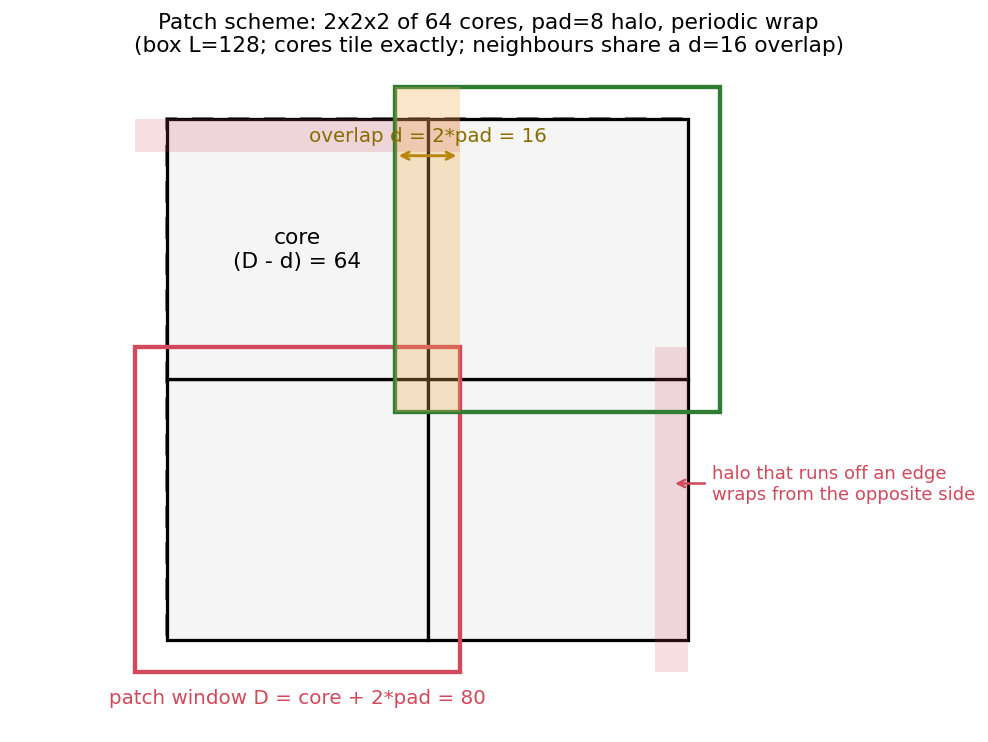
\includegraphics[width=0.82\linewidth]{figures_cmass/pipeline_patching.png}
\caption{Patch scheme. The box is cut into a $2{\times}2{\times}2$ grid of
$64^3$ cores that tile it exactly. With \texttt{pad}${>}0$ each patch is grown by
a halo of real neighbour cells (periodic wrap); only the central core is kept
and placed back.}
\label{fig:srs-patching}
\end{figure}

\paragraph{Per-simulation item.} Indexed by simulation, the dataset returns, for
all $8$ cores at once: the LR patches \texttt{lr\_in} of shape
$(8,\,1,\,64{+}2\,\texttt{pad},\,\cdot,\,\cdot)$ in model space, the HR cores
\texttt{hr\_tgt} of shape $(8,\,1,\,64,\,64,\,64)$, the style $\mathbf s$, and
the simulation index. The trainer flattens the $8$-core axis into the batch.

\begin{algorithm}[H]
\caption{\textsc{ExtractPatches} (one simulation)}
\label{alg:srs-extract}
\begin{algorithmic}[1]
\Require LR box $\mathbf L\in\mathbb R^{1\times128^3}$, HR box $\mathbf H$, \texttt{pad}
\State map $\mathbf L,\mathbf H$ to model space via Eq.~\ref{eq:srs-transform}
\For{$p=0,\dots,7$}
  \State $(i,j,k)\gets\textsc{unravel}(p,(2,2,2))$ \Comment{core origin $(64i,64j,64k)$}
  \State $\mathbf L_p\gets$ core $p$ grown by \texttt{pad} on each face, periodic wrap \Comment{$(64{+}2\,\texttt{pad})^3$}
  \State $\mathbf H_p\gets$ bare core $p$ \Comment{$64^3$}
\EndFor
\State \Return $\{(\mathbf L_p,\mathbf H_p)\}_{p=0}^{7}$, style $\mathbf s$
\end{algorithmic}
\end{algorithm}

\subsection{Model: Input/Output Specification}
\textit{Implementation: \texttt{map2map/models/styled\_srsgan.py}
(\texttt{G\_correct}, \texttt{D\_const}).}

\paragraph{What the generator computes.} The generator is a
\textbf{same-resolution residual} network: it does not change the grid size, and
it predicts a correction that is \emph{added} to the input. In model space,
\begin{equation}
  \mathrm{SR} \;=\; \mathrm{LR} \;+\; G(\mathrm{LR},\,\mathbf s,\,\mathbf z),
  \label{eq:srs-residual}
\end{equation}
where $\mathbf s$ is the cosmology vector and $\mathbf z$ is an injected noise
field (see below). Inputs and outputs are listed in
Table~\ref{tab:srs-model-io}; the generator is run once per core (the $8$ cores
of a box form a batch).

\begin{table}[t]
\centering
\caption{Tensors consumed/produced by the generator \texttt{G\_correct} for one
core (batch dimension omitted). Here $D=64{+}2\,\texttt{pad}$.}
\label{tab:srs-model-io}
\begin{tabular}{lll}
\toprule
Symbol & Shape & Meaning \\
\midrule
$\mathbf x$ (\texttt{x})       & $(1,D,D,D)$ & LR patch, model space (input) \\
$\mathbf s$ (\texttt{style})   & $(5,)$      & cosmology vector \\
$\mathbf z$ (\texttt{noise\_list}) & $2\cdot\texttt{num\_blocks}$ cubes $(1,D,D,D)$ & injected noise; fixed at inference, random in training \\
$G(\cdot)$                     & $(1,D,D,D)$ & predicted residual $\delta$ (added to $\mathbf x$) \\
\bottomrule
\end{tabular}
\end{table}

\paragraph{Internal composition.} $G$ is a constant-resolution StyleGAN2-style
network (no up/down-sampling), built from:
\begin{enumerate}
  \item \texttt{block0}: a $1{\times}1{\times}1$ style-modulated convolution
  (\texttt{ConvStyled3d}) lifting the $1$-channel input to $c_0$ channels,
  followed by a leaky ReLU.
  \item \texttt{num\_blocks} ($=4$) constant-resolution H-blocks
  (\texttt{HBlock\_const}). Each block, in order: inject noise $\to$
  $3{\times}3{\times}3$ \texttt{ConvStyled3d} (periodic ``circular'' padding)
  $\to$ leaky ReLU $\to$ inject noise $\to$ $3{\times}3{\times}3$
  \texttt{ConvStyled3d} $\to$ leaky ReLU $\to$ a $1{\times}1{\times}1$ projection
  to the output channel, accumulated into a running output $y$. The final return
  is $\mathbf x + y$ (Eq.~\ref{eq:srs-residual}).
\end{enumerate}
The channel widths come from \texttt{chan\_base} ($=128$) halved per block and
clamped to $[64,512]$. Two mechanisms make the convolutions depend on side
information:
\begin{itemize}
  \item \textbf{Style modulation.} \texttt{ConvStyled3d} is the StyleGAN2
  modulated/demodulated convolution: the cosmology vector $\mathbf s$ scales the
  convolution weights, so the same network behaves differently for different
  cosmologies. This is the only path by which $\mathbf s$ enters.
  \item \textbf{Noise injection.} Each \texttt{ConvStyled3d} is preceded by a
  per-channel learned-standard-deviation noise add (\texttt{\_NoiseInject}). At
  training time the noise is fresh Gaussian each call; at inference a
  \emph{fixed} list of noise cubes (seeded, built by \texttt{build\_noise\_list})
  is reused so outputs are reproducible. The noise is what lets the model produce
  a plausible small-scale field rather than a single blurred guess.
\end{itemize}

\paragraph{Discriminator.} \texttt{D\_const} is a constant-input-resolution
critic conditioned on the same style $\mathbf s$. It runs a head
\texttt{ConvStyled3d} then \texttt{num\_blocks} strided down-blocks (each a
periodic $3{\times}3{\times}3$ \texttt{ConvStyled3d} $+$ leaky ReLU $+$
$2{\times}$ average pool), a $1{\times}1{\times}1$ tail, and a final
$1{\times}1{\times}1$ projection to one channel, averaged over space to a single
logit per core.

\subsection{Training Step}
\textit{Located in: \texttt{train\_patch\_cmass.py}.}

The generator is trained per core (stitching is \emph{not} part of the
gradient). The total generator loss is a weighted sum of three terms,
\begin{equation}
  \mathcal L_G \;=\; \lambda_\text{adv}\,\mathcal L_\text{adv}
                  + \lambda_\text{rec}\,\mathcal L_\text{rec}
                  + \lambda_\text{pk}\,\mathcal L_\text{pk},
  \label{eq:srs-lossG}
\end{equation}
with (defaults from the original run script; see the protocol update below for
the values now in use):
\begin{itemize}
  \item \textbf{Reconstruction} $\mathcal L_\text{rec}=\lVert \mathrm{SR}-\mathrm{HR}\rVert_1$,
  a plain $L_1$ in model space (optionally Gaussian-smoothed; smoothing off in
  all runs).
  \item \textbf{Power-spectrum} $\mathcal L_\text{pk}$, the mean-squared error
  between the $\log_{10}$ power spectra of SR and HR, computed on the
  \emph{physical-count overdensity} of the $64^3$ core (Eqs.~\ref{eq:srs-transform}--\ref{eq:srs-delta}),
  Hann-windowed, with the HR side detached:
  \begin{equation}
    \mathcal L_\text{pk} = \frac{1}{|K|}\sum_{k\in K}
      \big(\log_{10} P_\text{SR}(k) - \log_{10} P_\text{HR}(k)\big)^2 .
    \label{eq:srs-pkloss}
  \end{equation}
  \item \textbf{Adversarial} $\mathcal L_\text{adv}=\mathrm{softplus}\!\big({-}D(\mathrm{SR},\mathbf s)\big)$,
  the non-saturating GAN generator loss.
\end{itemize}

\paragraph{Protocol update: what region the reconstruction and adversarial
terms see.} A \texttt{--pad-loss} setting controls how much of the generator's
output the $L_1$ and adversarial terms are computed on, independent of
\texttt{pad} itself:
\begin{itemize}
  \item \texttt{crop} (trim-aware, the setting used for Arm B above): the loss
  is computed only on \textsc{cropInterior}$(G(\mathbf x,\mathbf s),\,\texttt{pad})$,
  the $64^3$ core that is actually kept at inference time, against the bare
  $64^3$ HR core. The model is trained on exactly the region it will be graded
  on.
  \item \texttt{full}: the loss is computed on the whole $(64{+}2\,\texttt{pad})^3$
  output, against a correspondingly padded HR target (the dataset's
  \texttt{pad\_target} option). The model is trained as if the halo region it
  will later be trimmed off also mattered.
\end{itemize}
Concretely, let $\texttt{loss\_crop}=\texttt{pad}$ under \texttt{crop} and $0$
under \texttt{full}; every place above that writes $\mathrm{SR}$ means
$\textsc{cropInterior}(G(\mathbf x,\mathbf s),\,\texttt{loss\_crop})$, and the
Hann window and $P(k)$ estimator in $\mathcal L_\text{pk}$ are sized to match.
This is a controlled test of two ways padding could fail to help: see the
protocol-update subsection below for the result.

The discriminator is trained with the non-saturating GAN loss plus a lazy $R_1$
gradient penalty applied every \texttt{r1\_every} steps:
\begin{equation}
  \mathcal L_D = \mathrm{softplus}\!\big({-}D(\mathrm{HR})\big)
               + \mathrm{softplus}\!\big(D(\mathrm{SR})\big)
               + \tfrac{1}{2}\lambda_{R_1}\,\mathbb E\big\lVert \nabla_{\!x} D(x,\mathbf s)\big\rVert^2 .
  \label{eq:srs-lossD}
\end{equation}

\begin{algorithm}[H]
\caption{CMASS patch-GAN training step (one batch of cores)}
\label{alg:srs-train}
\begin{algorithmic}[1]
\Require LR patches $\mathbf x$, HR targets $\mathbf h$ (padded iff \texttt{pad-loss=full}),
         style $\mathbf s$, \texttt{pad}, \texttt{loss\_crop} ($=\texttt{pad}$ if \texttt{crop} else $0$),
         weights $\lambda_\text{adv},\lambda_\text{rec},\lambda_\text{pk},\lambda_{R_1}$
\Statex \textbf{// Discriminator}
\State $\hat{\mathbf h}\gets \textsc{cropInterior}\big(G(\mathbf x,\mathbf s),\,\texttt{loss\_crop}\big)$ \Comment{no grad}
\State $\mathcal L_D \gets \mathrm{softplus}({-}D(\mathbf h,\mathbf s)) + \mathrm{softplus}(D(\hat{\mathbf h},\mathbf s))$
\If{step $\bmod\ \texttt{r1\_every} = 0$} $\mathcal L_D \mathrel{+}= \tfrac12\lambda_{R_1}\texttt{r1\_every}\cdot R_1(D,\mathbf h,\mathbf s)$ \EndIf
\State update $D$ (Adam, grad-clip)
\Statex \textbf{// Generator}
\State $\hat{\mathbf h}\gets \textsc{cropInterior}\big(G(\mathbf x,\mathbf s),\,\texttt{loss\_crop}\big)$
\State $\mathcal L_\text{adv}\gets \mathrm{softplus}({-}D(\hat{\mathbf h},\mathbf s))$
\State $\mathcal L_\text{rec}\gets \lVert \hat{\mathbf h}-\mathbf h\rVert_1$
\State $\mathcal L_\text{pk}\gets$ Eq.~\ref{eq:srs-pkloss} on Hann-windowed overdensity of $\hat{\mathbf h}$, $\mathbf h$
       (skip if $\lambda_\text{pk}{=}0$)
\State $\mathcal L_G \gets \lambda_\text{adv}\mathcal L_\text{adv}+\lambda_\text{rec}\mathcal L_\text{rec}+\lambda_\text{pk}\mathcal L_\text{pk}$
\State update $G$ (Adam, grad-clip)
\end{algorithmic}
\end{algorithm}

\paragraph{Validation and checkpoint selection.} After each epoch we stitch the
full $128^3$ SR box for up to $40$ validation sims and report the stitched
$L_1$/voxel and the stitched-$128$ power-spectrum RMS against HR
(\S\ref{sec:srs-eval}, Eq.~\ref{eq:srs-pkrms}). A \texttt{--select} setting
chooses which of the two the saved \texttt{best.pt} tracks: \texttt{pk} (the
original setting, lowest stitched validation Pk RMS) or \texttt{l1} (lowest
stitched validation $L_1$/voxel). Selection is always on the stitched full box,
not the per-core training loss. Runs that also train with $\lambda_\text{pk}{=}0$
use \texttt{--select l1}, since selecting on Pk RMS while not training on it
would reintroduce the same metric leak in a different place.

\subsection{Inference}
\textit{Located in: \texttt{infer\_stitch\_cmass.py}.}

For one simulation: load the LR $128^3$ count box, map it to model space, run $G$
on each of the $8$ cores (with the periodic-wrap halo in Arm B), crop the halo,
stitch the cores into a $128^3$ model-space box, invert the transform to physical
counts, and clamp. \SG{are all outputs later mapped to integers, or are we fine with non-integer number of halos?} The injected noise list is fixed (seeded) so the output is
reproducible.

\begin{algorithm}[H]
\caption{CMASS inference + stitch (one simulation)}
\label{alg:srs-infer}
\begin{algorithmic}[1]
\Require LR box $\mathbf L$, style $\mathbf s$, trained $G$, mode (naive/overlap), fixed noise $\mathbf z$
\State $\texttt{pad}\gets 0$ if naive else value from checkpoint ($8$)
\State map $\mathbf L$ to model space (Eq.~\ref{eq:srs-transform})
\For{$p=0,\dots,7$}
  \State $\mathbf x_p\gets$ patch $p$ (core grown by \texttt{pad}, periodic wrap)
  \State $\mathbf c_p\gets \textsc{cropInterior}\big(G(\mathbf x_p,\mathbf s,\mathbf z),\,\texttt{pad}\big)$ \Comment{$64^3$ core, model space}
\EndFor
\State $\mathbf S\gets \textsc{stitch}(\{\mathbf c_p\})$ \Comment{$128^3$, model space}
\State $\mathbf S\gets \exp(\mathbf S)-1$, clamp to $[0,\,C_\text{max}{=}200]$, replace NaN/Inf \Comment{physical counts}
\State \Return $\mathbf S$
\end{algorithmic}
\end{algorithm}

\subsection{Crop Stitching}

Stitching is \textbf{direct placement with no averaging}. Adjacent cores tile the
box exactly (stride $64$, no overlap between cores once the halo is dropped), so
each core's $64^3$ output is written straight into its slot. In Arm B the $80^3$
patch is corrected and only its central $64^3$ core is kept; the overlap halo is
context for the convolution, never written to the output.

\begin{algorithm}[H]
\caption{\textsc{Stitch} ($8$ cores $\to$ $128^3$)}
\label{alg:srs-stitch}
\begin{algorithmic}[1]
\Require cores $\{\mathbf c_p\}_{p=0}^{7}$, each $1\times64^3$
\State $\mathbf S\gets \mathbf 0\in\mathbb R^{1\times128^3}$
\For{$p=0,\dots,7$}
  \State $(i,j,k)\gets\textsc{unravel}(p,(2,2,2))$
  \State $\mathbf S[:,\,64i{:}64i{+}64,\,64j{:}\cdots,\,64k{:}\cdots]\gets \mathbf c_p$ \Comment{direct assignment}
\EndFor
\State \Return $\mathbf S$
\end{algorithmic}
\end{algorithm}

\subsection{Evaluation}
\label{sec:srs-eval}
\textit{Located in: \texttt{analysis/eval\_seam\_cmass.py},
\texttt{analysis/diag\_cmass.py}, \texttt{analysis/match\_stats\_cmass.py},
\texttt{analysis/power\_spectrum.py}, \texttt{inference/nde.py},
\texttt{evaluate.py}.}

We evaluate the SR field against HR at three levels: a seam check (does stitching
leave a join?), field statistics (does SR have the right structure?), and
cosmology (does SR give the same parameter posterior as HR?).

\paragraph{Power-spectrum summaries.} On the count overdensity (Eq.~\ref{eq:srs-delta})
we report the power spectrum $P(k)$, the transfer ratio, and the cross-coherence:
\begin{equation}
  T(k) = \frac{P_\text{SR}(k)}{P_\text{HR}(k)},
  \qquad
  r(k) = \frac{P_{\text{SR},\text{HR}}(k)}{\sqrt{P_\text{SR}(k)\,P_\text{HR}(k)}} .
  \label{eq:srs-Tr}
\end{equation}
$T(k)=1$ means SR has the right \emph{amount} of power at scale $k$ (amplitude);
$r(k)=1$ means SR has the structure in the right \emph{place} (phase). The
scalar power-spectrum error used for checkpoint selection and seam reporting is
the log-RMS over the resolved $k$-bins:
\begin{equation}
  \mathrm{PkRMS}_{\log_{10}} = \sqrt{\frac{1}{|K|}\sum_{k\in K}
    \big(\log_{10} P_\text{SR}(k) - \log_{10} P_\text{HR}(k)\big)^2 } .
  \label{eq:srs-pkrms}
\end{equation}

\paragraph{Seam diagnostic.} \texttt{eval\_seam\_cmass.py} bins the per-cell
count error $|{\mathrm{SR}-\mathrm{HR}}|$ by distance to the nearest core face
and forms a per-position error profile along each axis. The headline number is
the \textbf{$x{=}64$ internal-seam excess}: the error on the internal core
boundary plane divided by the interior error. A value near $1$ means stitching
leaves no seam. The box edge $x{=}0$ is a periodic-boundary control.

\paragraph{Field-match statistics.} \texttt{match\_stats\_cmass.py} reports, over
$16$ test boxes: the total-count ratio $\sum\mathrm{SR}/\sum\mathrm{HR}$, the
void fraction (cells $<0.5$), the real-space cell standard-deviation ratio
$\mathrm{std}(\mathrm{SR})/\mathrm{std}(\mathrm{HR})$ (a blur check), and the
cross-coherence $r(k)$ at large ($k<0.05$) and small ($k>0.2$) scales.

\paragraph{Cosmology (posterior consistency).} This is the strongest ``does SR
match HR'' test. We voxel-count $\to$ overdensity $\to$ $P(k)$ for every box, then
train a neural density estimator $q(\theta\mid P(k))$ on the training split using
\texttt{sbi} (\texttt{SNPE\_C} with a neural-spline-flow density estimator,
\texttt{inference/nde.py}); the summary is $\log_{10}P(k)$. We train one estimator
on HR ($q_\text{HR}$) and one on each SR arm ($q_\text{SR}$). For each test box we
draw $2000$ posterior samples from each, fit a Gaussian per parameter, and report
the per-parameter Gaussian KL (\texttt{evaluate.py}):
\begin{equation}
  \mathrm{KL}\big(\mathcal N(\mu_\text{HR},\sigma_\text{HR})\,\Vert\,\mathcal N(\mu_\text{SR},\sigma_\text{SR})\big)
  = \tfrac12\!\left[\log\frac{\sigma_\text{SR}^2}{\sigma_\text{HR}^2}
    + \frac{\sigma_\text{HR}^2+(\mu_\text{HR}-\mu_\text{SR})^2}{\sigma_\text{SR}^2} - 1\right].
  \label{eq:srs-kl}
\end{equation}
$\mathrm{KL}=0$ means SR gives the identical cosmology posterior to HR. The raw LR
field (no model), pushed through the same pipeline, is the control SR must beat.

We report this comparison in two forms, and it matters which is which:
\begin{itemize}
  \item \textbf{Cross-fidelity (primary).} $q_\text{SR}$ is trained on SR power
  spectra but \emph{evaluated on the HR} $P(k)$ of each test simulation, and
  compared to $q_\text{HR}$ evaluated on the same HR $P(k)$. This is the
  deployment scenario the project targets: HR simulations are too expensive to
  train an inference model on, so the inference model is trained on cheap SR
  output and must still work when applied to (HR-like) reality. The comparison
  against an LR-trained estimator on the same HR data measures whether sampling
  in HR space (SR) survives the distribution shift better than staying in LR
  space. This metric never appears in the training loss.
  \item \textbf{Own-data (secondary).} $q_\text{SR}$ trained and evaluated on SR
  vs $q_\text{HR}$ trained and evaluated on HR, each pipeline end-to-end on
  its own field type.
\end{itemize}

\subsection{Best-Run Configuration}
\textit{Run script: \texttt{scripts/train\_patch\_cmass.slurm}; checkpoints
\texttt{checkpoints/patch\_cmass\_\{A,B\}/best.pt}.}

Both arms use the identical configuration below; they differ only in \texttt{pad}
($0$ for Arm~A, $8$ for Arm~B). This is the configuration behind every number
in \S\ref{sec:srs-results}--\S\ref{sec:srs-next}.

\begin{lstlisting}[language=bash]
--transform log1p   --nbar perbox        # log(1+n) model space; per-box nbar
--epochs 30         --sims-per-batch 1    # patch-batch = 8 cores per step
--chan-base-g 128   --chan-base-d 64  --num-blocks 4
--lambda-adv 1.0    --lambda-rec 2.0  --lambda-pk 2.0   # generator weights
--lambda-r1 10.0    --r1-every 16                       # lazy R1
--lr-g 1e-4 --lr-d 1e-4  --beta1 0.0 --beta2 0.99       # Adam
--grad-clip 1.0     --val-max-sims 40    --select pk    # select on Pk RMS
\end{lstlisting}

The best checkpoint per arm is the one with the lowest stitched validation Pk RMS
(Eq.~\ref{eq:srs-pkrms}):

\begin{center}
\begin{tabular}{lc}
\toprule
arm & best stitched val PkRMS$_{\log_{10}}$ \\
\midrule
Arm A, naive (pad $0$)  & $0.0947$ \\
Arm B, overlap (pad $8$) & $0.0963$ \\
\bottomrule
\end{tabular}
\end{center}

\paragraph{Protocol update.} Following the mentor meeting reported in
\S\ref{sec:srs-followup}, the configuration above is no longer the one we train
with. Three settings changed:
\begin{lstlisting}[language=bash]
--lambda-pk 0.0      # power-spectrum term OFF (it was also our main metric)
--pad-loss crop|full # trim-aware vs trim-unaware padding, see below
--select l1          # select on stitched L1, not the term we removed
\end{lstlisting}
All results in \S\ref{sec:srs-followup} use this configuration. Runs under the
original configuration above (Arm A, Arm B, and everything derived from them in
\S\ref{sec:srs-results}--\S\ref{sec:srs-next}) remain valid as a record of that
protocol; they are superseded, not invalidated, by the update.

\subsection{Results: Does SR Match HR?}
\label{sec:srs-results}

All numbers are on the $200$-box test split unless noted.

\paragraph{1. Power spectrum (statistics).} Across the test set the SR power
spectrum tracks HR at every scale, and Arm A beats the no-model LR control on the
overall log-RMS (Fig.~\ref{fig:srs-srvshr}, computed by
\texttt{analysis/plot\_sr\_vs\_hr.py}).

\begin{table}[h]
\centering
\caption{SR vs HR power-spectrum agreement, $200$ test boxes. Transfer
$T(k)=P_X/P_\text{HR}$ (Eq.~\ref{eq:srs-Tr}); $1.0$ is perfect.}
\label{tab:srs-pk}
\begin{tabular}{lccc}
\toprule
field (vs HR) & PkRMS$_{\log_{10}}$ & $T$ at large scales ($k{<}0.1$) & $T$ at small scales ($k{>}0.3$) \\
\midrule
SR (Arm A, naive)    & $\mathbf{0.0607}$ & $0.95$ & $1.04$ \\
SR (Arm B, overlap)  & $0.0645$ & $0.93$ & $0.88$ \\
LR (no model, control) & $0.0641$ & $1.01$ & $1.01$ \\
\bottomrule
\end{tabular}
\end{table}

\begin{figure}[t]
\centering
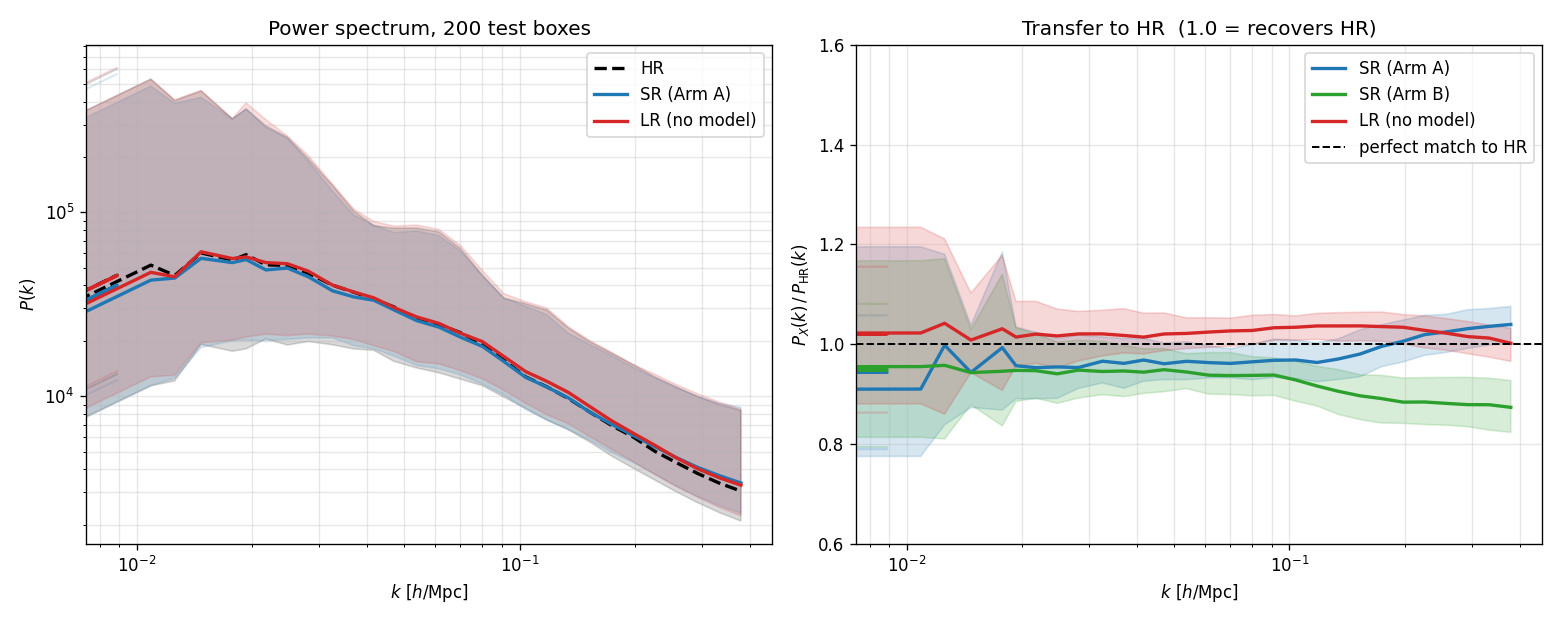
\includegraphics[width=0.98\linewidth]{figures_cmass/sr_vs_hr_pk.png}
\caption{\textbf{Left:} $P(k)$ of HR, SR (Arm A), and LR over $200$ test boxes
(median $+$ $16/84\%$ band). \textbf{Right:} transfer to HR; $1.0$ recovers HR.
SR (Arm A) sits near $1$ at all scales; Arm B's overlap blending slightly
suppresses small-scale power (transfer $0.88$).}
\label{fig:srs-srvshr}
\end{figure}

\paragraph{2. Field structure.} Beyond the power spectrum, SR keeps the field
structure of HR (Arm A, $16$ test boxes, \texttt{match\_stats\_cmassA.txt}):

\begin{table}[h]
\centering
\caption{SR vs HR field-match statistics (Arm A).}
\label{tab:srs-match}
\begin{tabular}{lll}
\toprule
quantity & value & reading \\
\midrule
total count ratio $\sum\mathrm{SR}/\sum\mathrm{HR}$ & $0.965\pm0.172$ & counts conserved on average; large per-box scatter \\
real-space std ratio & $1.008\pm0.100$ & clustering amplitude matches; not blurred \\
void fraction SR / HR ($<0.5$) & $0.855$ / $0.833$ & SR keeps voids empty, like HR \\
cross-coherence $r$, $k<0.05$ & $0.951$ & large-scale structure matches cell-by-cell \\
cross-coherence $r$, $k>0.2$ & $0.403$ & small-scale structure decorrelates \\
\bottomrule
\end{tabular}
\end{table}

\paragraph{3. Cosmology.} The cosmology comparison in the original report used
mislabeled cosmologies, an indexing bug we describe and fix in
\S\ref{sec:srs-correction}, so those numbers are not shown here. With correct
labels a single box constrains $\Omega_m$ and $\sigma_8$; at the power spectrum
level the raw LR field is already HR-like, while at the field level an SR-trained
posterior transfers to HR and an LR-trained one does not
(\S\ref{sec:srs-correction}, Table~\ref{tab:srs-corrected}).

\paragraph{4. Seam.} Neither arm introduces a stitching seam: the $x{=}64$
internal-seam excess is $\approx1$ for both
(Table~\ref{tab:srs-seam}, Fig.~\ref{fig:srs-seam}). Arm A shows a mild generic
ripple near \emph{any} boundary plane (seam-distance ratio $1.17$); Arm B's
overlap removes it ($1.00$) at a small cost in Pk RMS.

\begin{table}[h]
\centering
\caption{Seam and stitched-fidelity metrics, $200$ test boxes. ``Excess'' is
boundary error over interior error; $\approx1$ means no seam.}
\label{tab:srs-seam}
\begin{tabular}{lccp{5.2cm}}
\toprule
metric & Arm A naive & Arm B overlap & reading \\
\midrule
$x{=}64$ internal-seam excess & $0.9934$ & $0.9998$ & no internal seam either arm \\
seam-distance ratio ($d{=}0/d{\ge}8$) & $1.1729$ & $1.0032$ & generic boundary ripple, removed by overlap \\
$x{=}0$ periodic edge (control) & $0.9930$ & $0.9993$ & box edge behaves like interior \\
stitched PkRMS$_{\log_{10}}$ vs HR & $0.0637$ & $0.0678$ & stitched power-spectrum match \\
\bottomrule
\end{tabular}
\end{table}

\begin{figure}[t]
\centering
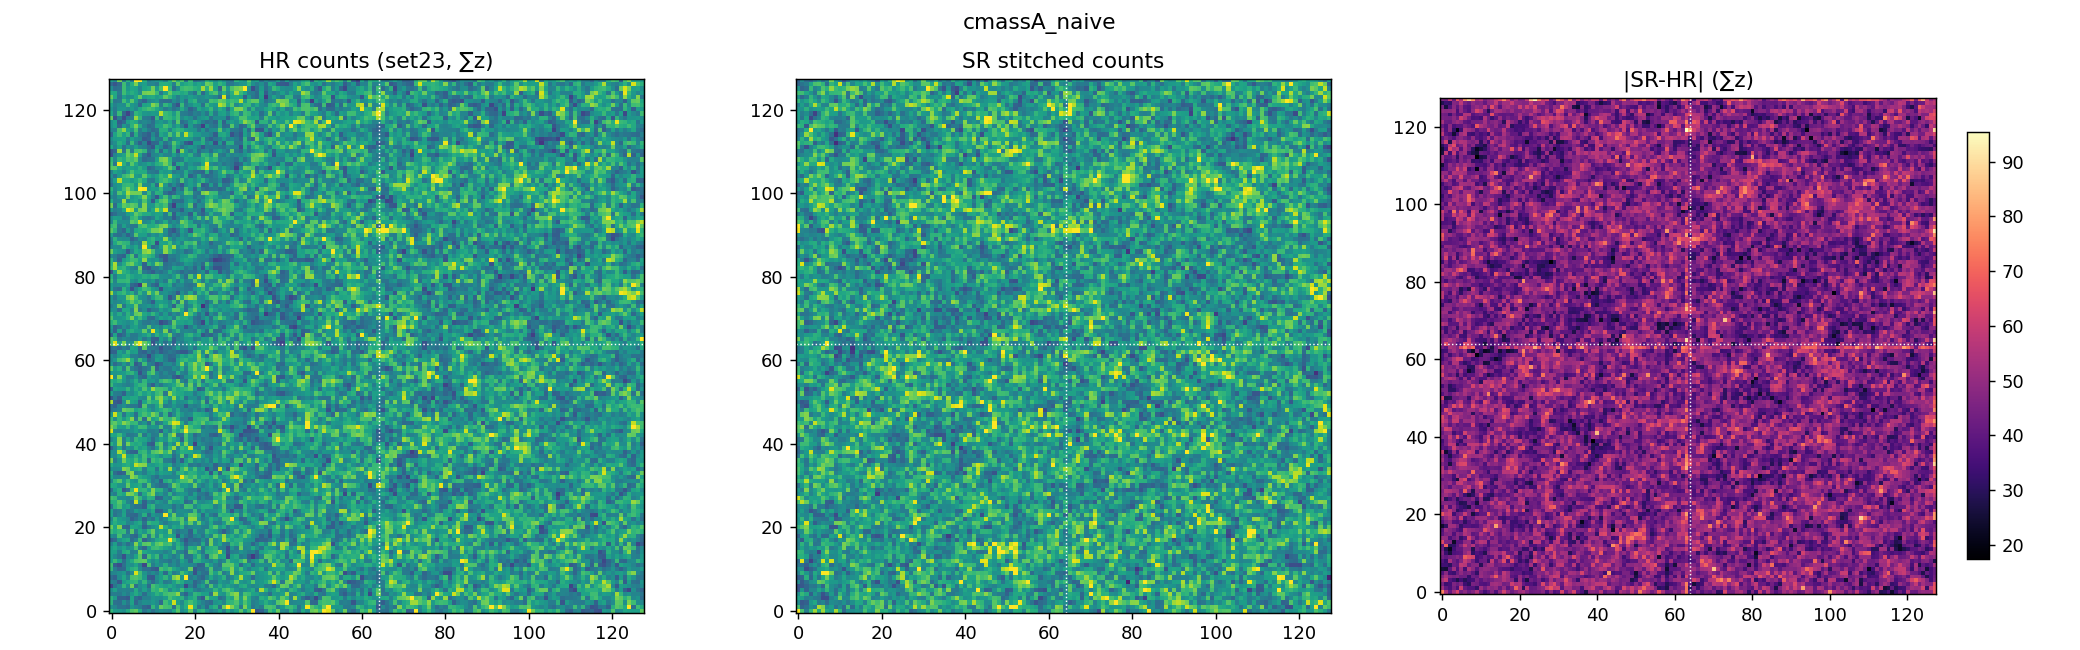
\includegraphics[width=0.95\linewidth]{figures_cmass/seam_cmassA_naive_slice.png}
\caption{Projected count maps for one test box (Arm A): HR, stitched SR, and the
absolute residual $|\mathrm{SR}-\mathrm{HR}|$. White dotted lines mark the
$x{=}64$, $y{=}64$ core boundaries; the residual shows no elevated ridge along
them.}
\label{fig:srs-seam}
\end{figure}

\paragraph{Per-scale diagnostic panels.} Figure~\ref{fig:srs-pkpanel} shows the
full-box $P(k)$, transfer, and cross-coherence for Arm A. The transfer sits near
$1$ at all scales (right amount of power); the cross-coherence is near $1$ at
large scales and falls toward small scales (structure placement is recovered at
large scales only). The per-patch panel
(\texttt{figures\_cmass/pk\_panel\_patch\_cmassAfix.png}) and the projection panels
(\texttt{projection\_box\_cmassAfix\_set23.png},
\texttt{projection\_patch\_cmassAfix\_set23\_p0.png}) tell the same story; Arm~B's
panels carry the \texttt{cmassB} suffix.

\begin{figure}[t]
\centering
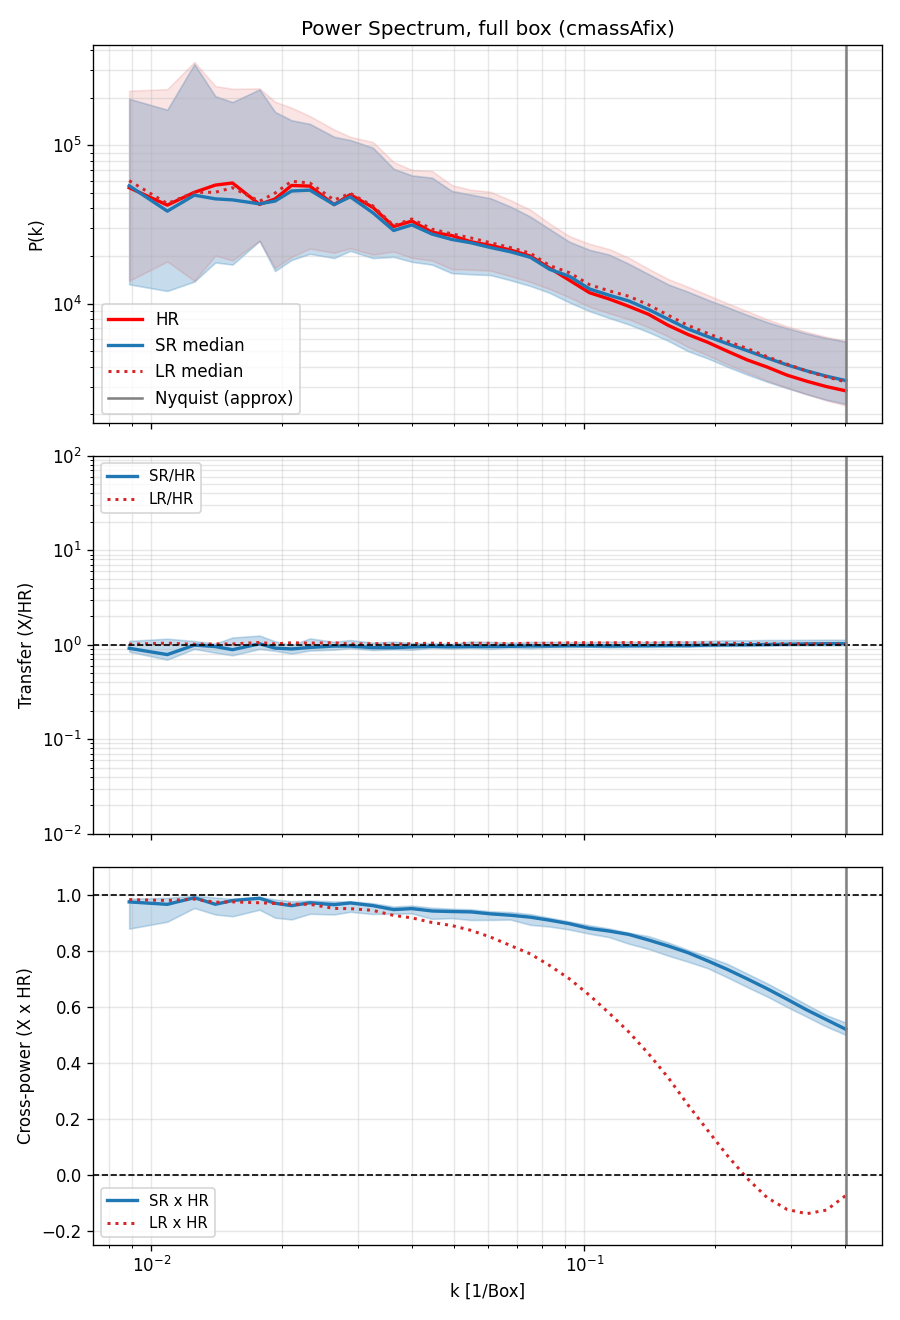
\includegraphics[width=0.5\linewidth]{figures_cmass/pk_panel_box_cmassAfix.png}
\caption{Full-box diagnostic for the conditioned generator (fiducial cosmology,
$16$ test boxes): $P(k)$ of HR (red), SR (blue median $+$ band), and LR (dotted
red); transfer $T(k)=P_X/P_\text{HR}$ on a linear axis with the 16 to 84
percentile band for both SR and LR, the legend reporting the RMS deviation of
each ratio from unity; and cross-coherence $r(k)$. The SR median transfer sits
below unity for $k<0.1$, a systematic large-scale power deficit of roughly 5 to
10 percent, while LR sits slightly above unity; SR does not tighten the transfer
scatter relative to LR. In $r(k)$, SR stays near unity to smaller scales while
LR decorrelates.}
\label{fig:srs-pkpanel}
\end{figure}

\subsection{Diagnostic: What is NOT Working}

\paragraph{Small-scale structure decorrelates, and this is fundamental.} SR
matches HR cell-by-cell at large scales ($r{=}0.95$ for $k<0.05$) but loses the
match at small scales ($r{=}0.40$ for $k>0.2$, Table~\ref{tab:srs-match}). This
is not a capacity bug: it is set by how much information the LR input carries
about HR. LR and HR share large-scale modes but the voxel-by-voxel LR$\leftrightarrow$HR
correlation is only $\approx0.06$, so the exact small-scale realization is simply
not present in the input. The model can match the small-scale \emph{statistics}
(transfer $\approx1$, real-space std ratio $1.008$) but cannot reproduce the
exact placement of individual halos. The noise injection
(Eq.~\ref{eq:srs-residual}) exists precisely because of this: it draws a
plausible small-scale field rather than regressing to a blur.

\paragraph{Per-box total-count scatter.} The total halo count is conserved on
average but with $\sim17\%$ per-box scatter ($\sum\mathrm{SR}/\sum\mathrm{HR}=
0.965\pm0.172$). A count-aware output head (predict a rate and sample Poisson
counts) would tighten this; it is the one clearly addressable imperfection. \SG{I would think this isn't necessary to fix, we don't care about the number of halos after all.}

\paragraph{Overlap suppresses small-scale power.} Arm B's overlap blending lowers
the small-scale transfer to $0.88$ (Table~\ref{tab:srs-pk}), so on the power
spectrum the naive Arm A is the better super-resolver. Overlap removes a small
generic boundary ripple but buys no fidelity, because on this continuous count
data there is no real seam to fix, the clean version of the mentor 2.1 vs 2.2
comparison.

\paragraph{Where the cosmology value is.} At the power spectrum level the raw LR
field is already close to HR, since they share large-scale modes, so the power
spectrum is a forgiving summary with little headroom. The model's value is at the
field level (variance, voids, small-scale structure), which the power spectrum
summary is insensitive to. The corrected cross-fidelity in
\S\ref{sec:srs-correction} bears this out: SR and LR are indistinguishable at the
power spectrum level, but at the field level an SR-trained posterior transfers to
HR while an LR-trained one does not.

\subsection{What I'm Trying Next}
\label{sec:srs-next}

The diagnostics above point to one limit that may be fundamental (small-scale
decorrelation) and a few that are clearly fixable (count scatter, small-scale
realism). The plan below is ordered so that we \emph{measure} the limit before
spending effort trying to beat it. None of these results are in yet; this is the
roadmap, not an experiment log.

\paragraph{Step 0, measure the information ceiling first.} Before trying to
improve the small-scale match, we need to know whether $r{=}0.40$ at small scales
(Table~\ref{tab:srs-match}) is the best any model could do from this input, or a
weakness of the current one. Two cheap diagnostics settle it:
\begin{itemize}
  \item \textbf{LR$\leftrightarrow$HR cross-coherence $r_\text{LR,HR}(k)$.} The
  cross-coherence of the \emph{raw input} against HR (no model) is the ceiling:
  no function of LR can place small-scale structure better than the input
  already correlates with HR. If $r_\text{SR,HR}(k)\approx r_\text{LR,HR}(k)$ at
  small $k$, the model is already at the ceiling and the limit is fundamental;
  if it sits well below, there is recoverable structure left on the table. (Only
  per-box $P(k)$ is currently saved, not the cross-spectrum, so this needs one
  re-run that keeps the fields.)
  \item \textbf{No-noise ablation.} Train the same generator with the noise
  injection off (a plain regressor). Theory predicts this should \emph{raise} the
  small-scale cross-coherence a little (a regressor targets the conditional mean,
  the best cell-by-cell predictor) but \emph{lower} the small-scale transfer well
  below $1$ (the conditional mean is blurry). Seeing exactly that trade-off would
  confirm that the noise/GAN is the right choice for a power-spectrum target, and
  would quantify how much cell-by-cell accuracy is being traded for correct
  statistics.
\end{itemize}

\paragraph{Step 1, fix the count scatter and small-scale realism (independent
of the ceiling).} These help regardless of what Step 0 finds:
\begin{itemize}
  \item \textbf{Count-aware (Poisson) output head.} Instead of predicting a
  count directly, predict a non-negative rate $\lambda$ per cell and sample the
  count as $n\sim\mathrm{Poisson}(\lambda)$. Halo counts are discrete and sparse,
  so a Poisson head models the small-scale graininess as actual shot noise rather
  than a smeared residual, and should tighten the $\sim17\%$ per-box total-count
  scatter (Table~\ref{tab:srs-match}), the one clearly addressable imperfection.
  \item \textbf{Explicit statistics terms in the loss.} Add a one-point PDF /
  variance matching term so small-scale sharpness is enforced directly, rather
  than relying on the adversarial term alone to find it.
  \item \textbf{Loss rebalance.} The current weights are $\lambda_\text{rec}{=}2$,
  $\lambda_\text{pk}{=}2$, $\lambda_\text{adv}{=}1$
  (Eq.~\ref{eq:srs-lossG}). The $L_1$ term blurs; lowering it and raising the
  adversarial weight should push toward correct statistics, at a known cost in
  cell-by-cell accuracy, per the same trade-off as the no-noise ablation.
\end{itemize}

\paragraph{Step 2, extract more of the available information (only if Step 0
shows headroom).} If $r_\text{SR,HR}$ sits below the LR$\leftrightarrow$HR
ceiling, the model is under-using its input. A larger receptive field, or feeding
each patch more neighbour context, would let it use more of the LR field to
predict the residual. This only helps if there is headroom to recover.

\paragraph{Step 3, raise the ceiling by changing the \emph{input}, not the
model.} The small-scale cell-by-cell limit is set by the information in the LR
input (the voxel-by-voxel LR$\leftrightarrow$HR correlation is only
$\approx0.06$). No amount of model capacity raises that; only more informative
inputs do. Candidates: feed the shared small-scale \emph{initial conditions}
(which the coarse LR count field has discarded), or add the LR velocity / particle
fields. This is the only route to a meaningful gain in small-scale cross-coherence,
and is the natural bridge to the displacement-field model of \S5, which already
carries that extra information.

\paragraph{Summary.} Steps 0--1 are the near-term plan: measure the ceiling, then
add a Poisson head and statistics losses to fix the count scatter and sharpen the
small-scale field. Steps 2--3 are contingent on what Step 0 reveals. For a
cosmology deliverable the priority is statistical fidelity (which Steps 0--1
target); exact small-scale reconstruction (Step 3) is a larger, input-level
change worth it only if cell-by-cell recovery becomes the goal.

\subsection{Follow-Up Results: New Protocol from the Mentor Meeting}
\label{sec:srs-followup}

A mentor meeting after the report above changed two things about how we train
and evaluate this model. First, the real goal is not to match HR with SR by
itself. The real goal is to train a posterior model on SR output and have it
work well when it is tested on real HR data, since HR simulations are too
expensive to train a posterior model on directly. Second, the power spectrum
term was removed from the training loss, since it was also our main success
metric and that is a weak test. This subsection reports what we found. Some of
the training runs below are still in progress at the time of writing, so
numbers marked as current are read from the latest completed epoch, not a
final result.

\paragraph{Held-out check: the bispectrum.} A fair worry is that our power
spectrum result looks good only because the power spectrum was also in the
training loss. To check this we measured the bispectrum, a higher-order
statistic that was never used anywhere in training or model selection. If SR
only matches the power spectrum and nothing else, the bispectrum should show
no improvement over the raw LR input.

\begin{figure}[t]
\centering
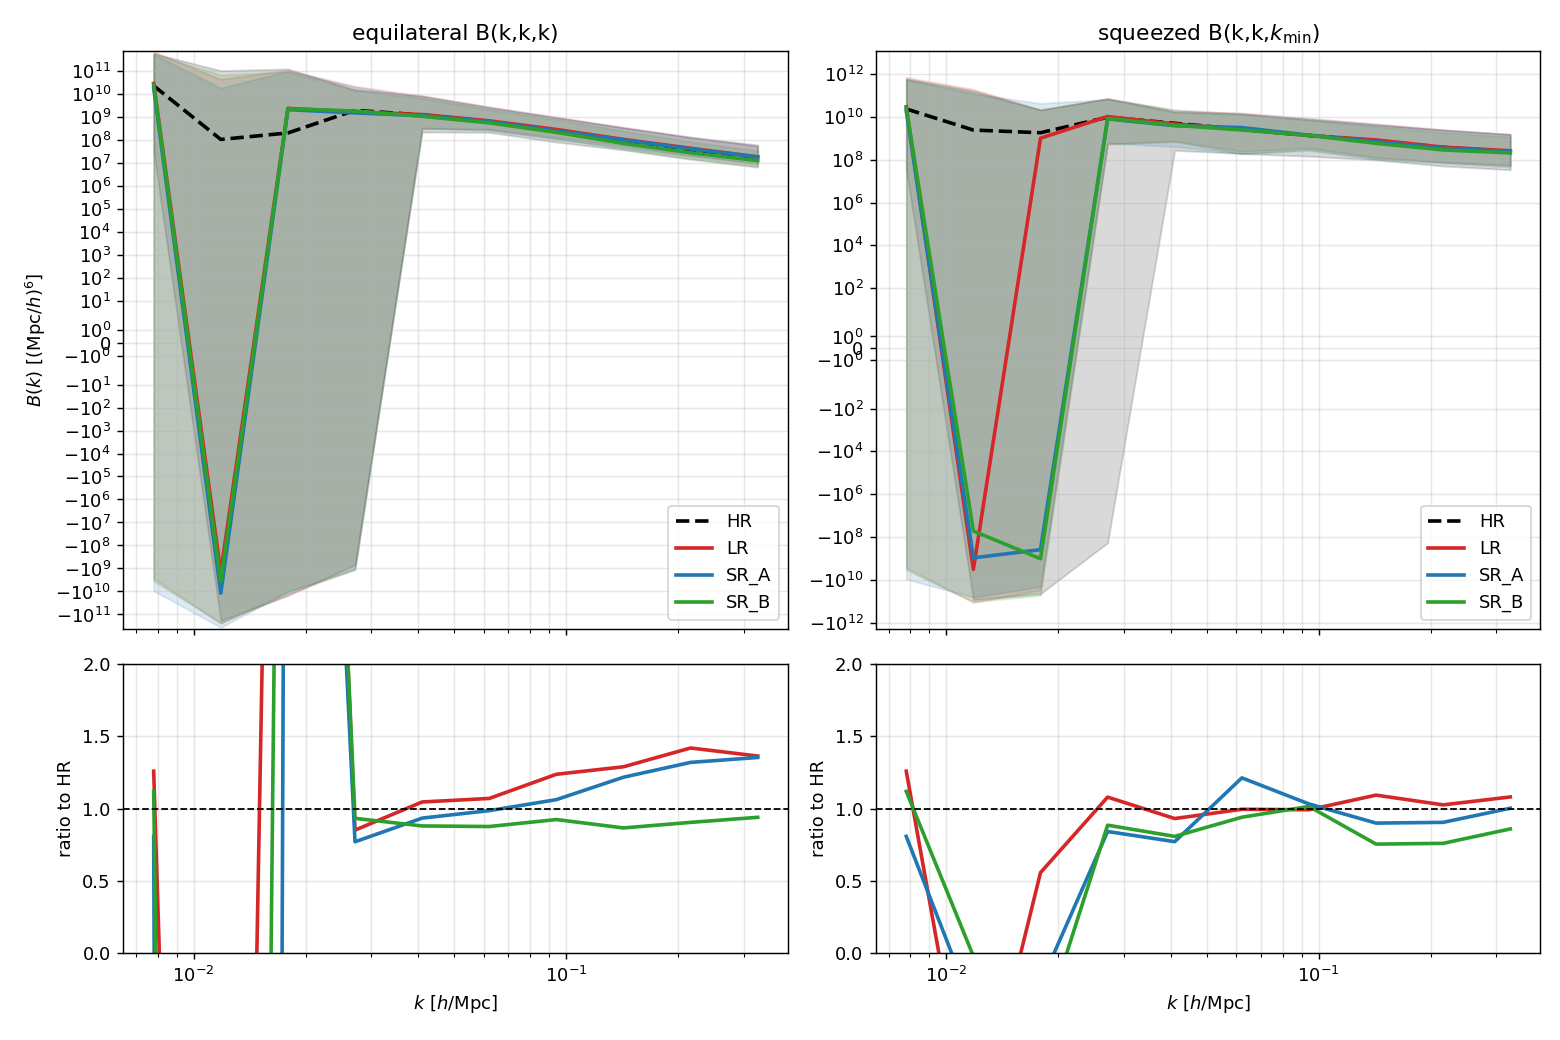
\includegraphics[width=0.95\linewidth]{figures_cmass/bispectrum_hr_lr_srA_srB.png}
\caption{Bispectrum of HR, LR, and SR (both arms), on $16$ test boxes. Top:
equilateral and squeezed bispectrum, HR in black. Bottom: ratio to HR. SR
removes most of the systematic excess that LR has at the plotted scales,
without ever training on this statistic.}
\label{fig:srs-bispec}
\end{figure}

On the equilateral configuration, LR sits about $6$ to $13$ percent above HR
across the middle range of scales. SR removes most of this gap without ever
seeing a bispectrum during training, and it does this for both arms. This is
evidence that the model is not simply fitting the training metric. It is
correcting real structure in the field that also shows up in a statistic it
never saw. (The figure uses the earlier models trained \emph{with} the power
spectrum loss; the no-Pk models of the following paragraphs preserve the
bispectrum at least as well, so removing that loss did not degrade this
held-out statistic either.)

\paragraph{Removing the power spectrum loss.} Following the meeting, we
retrained the model with the power spectrum term switched off
($\lambda_\text{pk}{=}0$ in Eq.~\ref{eq:srs-lossG}), so the loss is only the
adversarial and $L_1$ terms. We also changed which checkpoint counts as "best"
to the real-space $L_1$ error, since selecting on the power spectrum would
have been the same kind of leak we were trying to remove.

\begin{figure}[t]
\centering
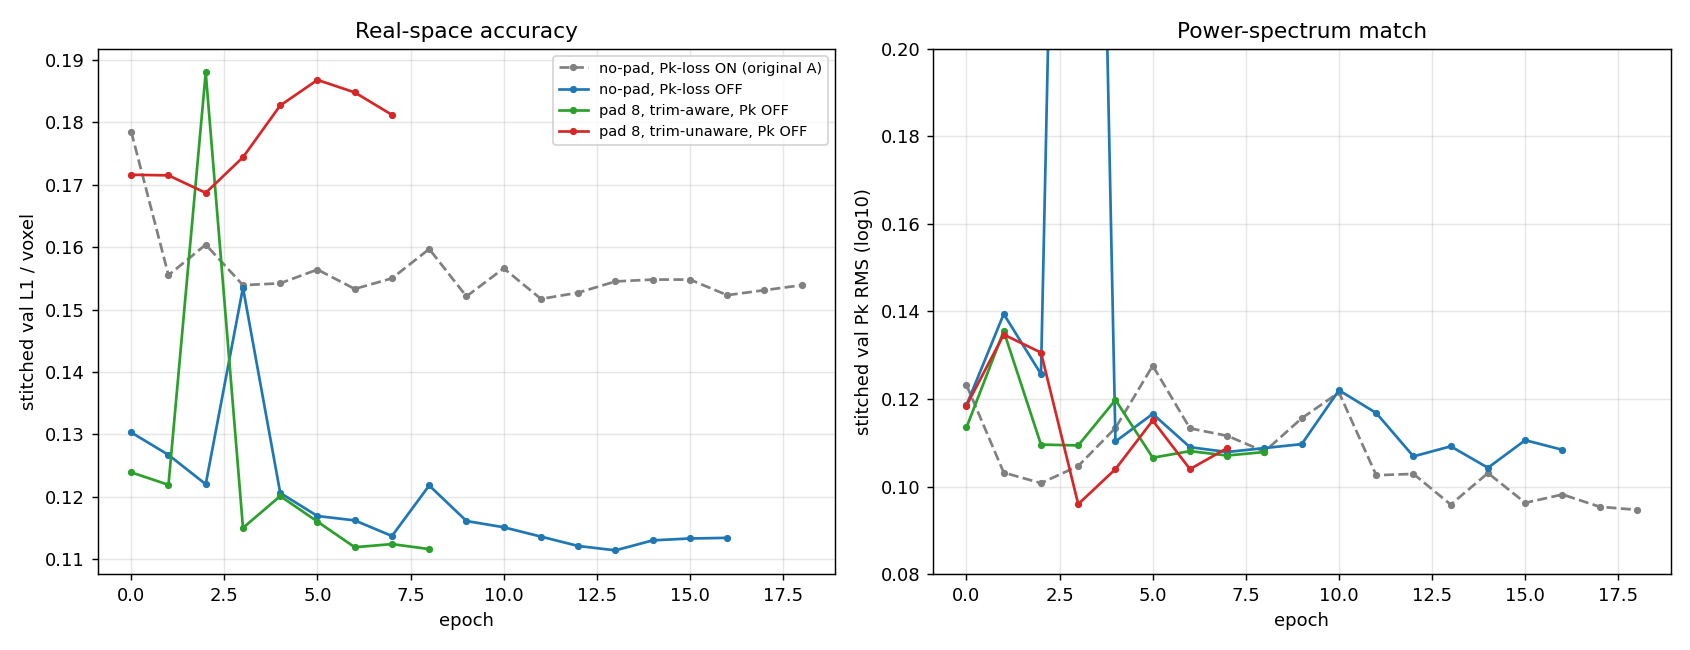
\includegraphics[width=0.98\linewidth]{figures_cmass/protocolv2_cmass.png}
\caption{Stitched validation curves under the new protocol (power spectrum
loss off). Left: real-space $L_1$ error. Right: power spectrum RMS error. Grey
dashed: the original Arm A with the power spectrum loss on, for comparison.
These runs are still training; curves stop at the most recent completed
epoch.}
\label{fig:srs-protocolv2}
\end{figure}

Two things stand out so far. First, without the power spectrum term, the
real-space $L_1$ error becomes clearly better than the original run at the
same point in training (left panel, blue and green curves sit below the grey
dashed curve). Second, the power spectrum error does get a little worse
without its loss term, but it does not collapse: it settles into roughly the
same range as before, just a bit noisier. So the power spectrum term was
buying us a small amount of power spectrum accuracy at a real cost in
real-space accuracy. It was not the only reason the power spectrum matched
well; the adversarial and reconstruction terms carry most of that on their
own.

\paragraph{Does padding help, once the power spectrum loss is out of the way?}
The report above found that padding (Arm B) did not beat no padding (Arm A) on
the power spectrum. The mentor pointed out two different ways this could
happen, and that they make different, testable predictions:
\begin{itemize}
  \item \textbf{Trim-aware.} The model is trained knowing that only the middle
  part of its output will be kept; the loss only looks at that middle part.
  This is what Arm B already did. If this is working correctly, padding should
  train at least as well as no padding, since it has strictly more context for
  the same target.
  \item \textbf{Trim-unaware.} The model is trained as if its whole padded
  output matters, including the edge region that gets thrown away later. If
  the model leans on that edge region during training, it should look fine
  during training but generalize worse once the edge is cut off at test time.
\end{itemize}
We trained both versions with the power spectrum loss off, so the comparison
is not confused by that term. Figure~\ref{fig:srs-protocolv2} shows all three
runs together (no padding, trim-aware padding, trim-unaware padding).

The trim-aware version (green) matches or beats no-padding (blue) on both
real-space error and power spectrum error at almost every epoch measured so
far. This supports the first prediction: once the model is told correctly what
part of its output is graded, more context helps rather than hurts. The
trim-unaware version (red) is clearly worse on real-space error than both
other runs, and does not close that gap as training continues. This supports
the second prediction: a model that is allowed to rely on the part of its
output that gets discarded at test time pays for that at test time. Put
together, the original result that padding did not help was most likely
caused by the power spectrum loss, not by padding itself.

We also reran the older, padding-with-power-spectrum-loss model for more
epochs to check whether it had simply not been trained long enough. Fifteen
additional epochs did not beat its early best score, so that run was not
undertrained; the training recipe, not the training time, was the limiting
factor.

\subsection{The Goal Metric: Corrected Cross-Fidelity Results}
\label{sec:srs-correction}

\paragraph{The bug.} After the analysis above, a routine physical sanity check
failed in a way that could not be real: the amplitude of the power spectrum had
essentially zero correlation with $\sigma_8$, and a fit of the power spectrum to
the five parameters explained only $0.2\%$ of the variance. The power spectrum
amplitude must scale with $\sigma_8$, so this pointed to a labeling error, not to
physics. Tracing it, we found that the processed count fields were written in
string-sorted simulation order ($0, 1, 10, 100, 1000, \dots$) while the cosmology
table is indexed numerically. Field number $k$ is therefore the halo field of
simulation string-sort$(k)$, not simulation $k$, so every field in the whole
pipeline was paired with the wrong cosmology. We proved this exactly: using the
original halo catalogs, the field halo count matches the catalog count under the
string-sort permutation for all $2000$ simulations, while the identity mapping
matches only the two fixed points. We corrected the cosmology table to field
order, backed up the old one, and patched the builder so it cannot regenerate the
wrong order.

\begin{figure}[h]
\centering
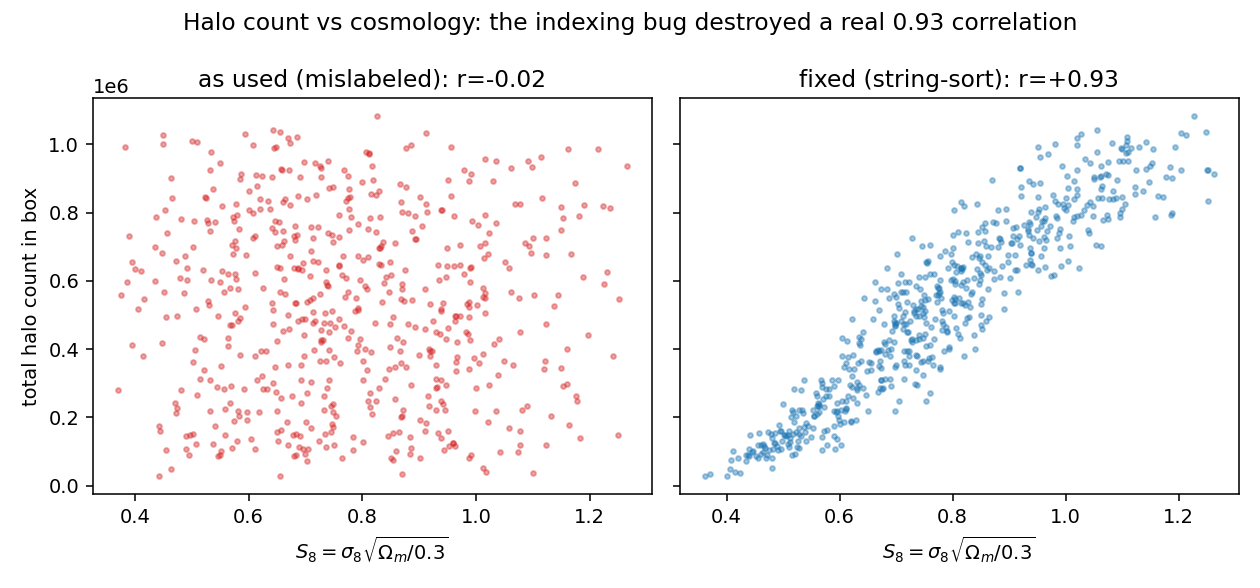
\includegraphics[width=0.85\linewidth]{figures_cmass/labelbug_count_vs_s8.png}
\caption{The indexing bug in one picture. Total halo count in a box against
$S_8 = \sigma_8\sqrt{\Omega_m/0.3}$. As the pipeline used the labels (left) the
correlation is zero; with the string-sort mapping corrected (right) the true
$0.93$ correlation reappears. Halo abundance must track $S_8$, so the left panel
was the signature of a labeling error, not of uninformative data.}
\label{fig:srs-labelbug}
\end{figure}

\paragraph{What this changes, and what it does not.} Every cosmology number we
computed before this point used the labels and is affected; the earlier
cross-fidelity tables have been removed and are replaced by the corrected results
below, and the earlier reading that the SR-versus-LR difference was an irreducible
coin flip was itself a product of the mislabeling. The results that do not use the
labels are unaffected and still stand: the power spectrum match of SR to HR, the
held-out bispectrum, the field-match statistics, the seam test, and the real space
error. The generator conditions on the cosmology as a style vector and was trained
with the scrambled labels, so its conditioning was uninformative during training;
we return to this at the end.

\paragraph{The data is informative after all.} With correct labels the picture
inverts. A halo count in this suite carries a strong cosmological signal: the
total halo count alone correlates with the combination $S_8 = \sigma_8
\sqrt{\Omega_m/0.3}$ at $0.93$ and with $\Omega_m$ at $0.85$. A Fisher forecast on
a single-box power spectrum now explains $98\%$ of the variance, where it
explained $0.2\%$ before, and it constrains $\Omega_m$ and $\sigma_8$ well, with
$\Omega_b$, $h$ and $n_s$ weak or unconstrained, which is the textbook pattern for
a low-redshift halo field. The field-level network tells the same story: after the
fix its predicted $\Omega_m$ correlates with the truth at $0.90$ on both training
and test boxes, where before the fix the correlation was zero and the output was a
constant. So the earlier conclusion that a single box carries almost no cosmology
was an artifact of the labeling, not a property of the data.

\begin{figure}[h]
\centering
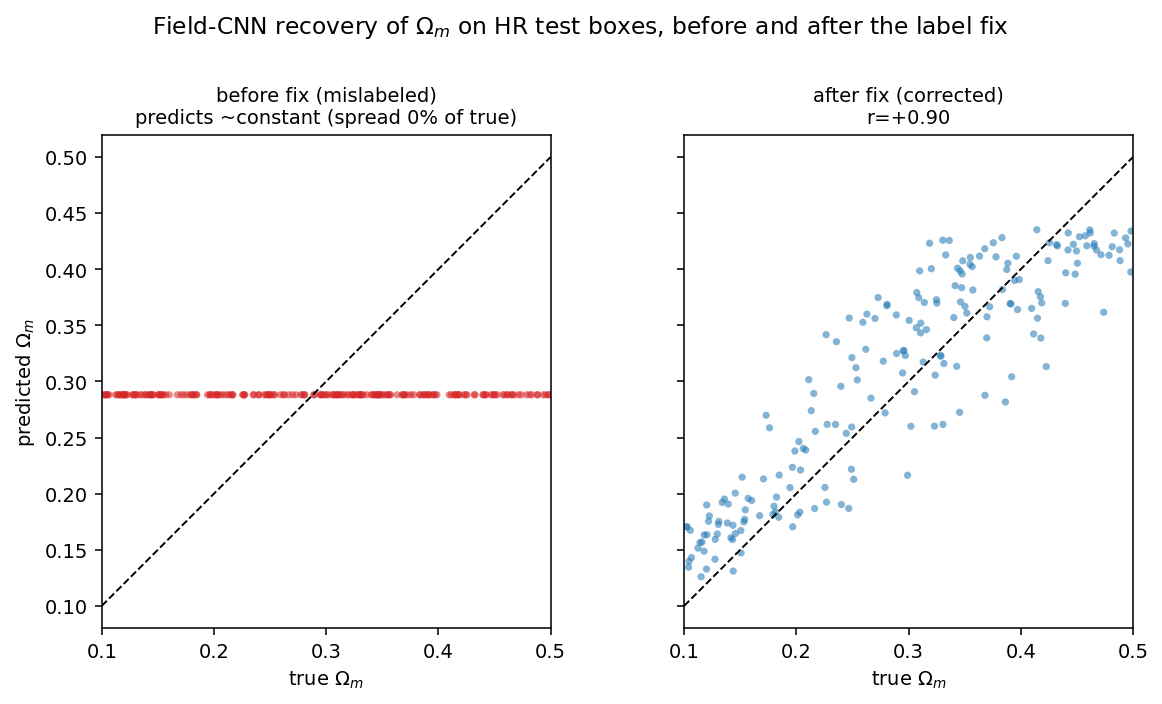
\includegraphics[width=0.82\linewidth]{figures_cmass/field_recovery_Om_cmass.png}
\caption{Field-level CNN recovery of $\Omega_m$ on HR test boxes, before and after
the label fix. Before (left) the prediction is flat and uncorrelated with the
truth (the network returns a near-constant); after (right) it tracks the diagonal
at a correlation of about $0.90$, on both training and test boxes. Same
architecture, same data, only the labels changed.}
\label{fig:srs-recovery}
\end{figure}

\begin{figure}[h]
\centering
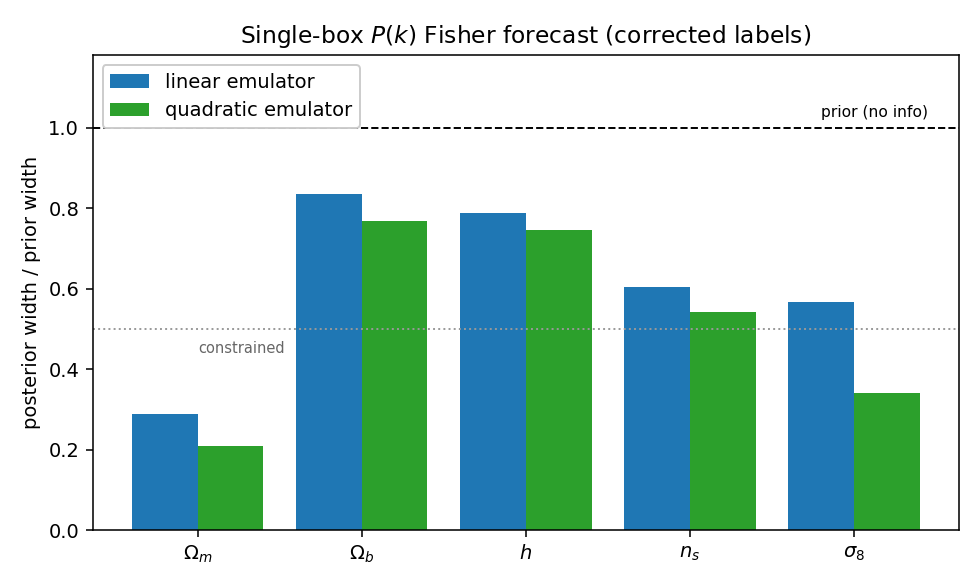
\includegraphics[width=0.72\linewidth]{figures_cmass/fisher_corrected_cmass.png}
\caption{Fisher forecast for a single-box power spectrum with corrected labels:
posterior width divided by prior width per parameter (lower means better
constrained, $1$ means no information). $\Omega_m$ is well constrained and
$\sigma_8$ is constrained, while $\Omega_b$, $h$ and $n_s$ are weak, the textbook
pattern for a low-redshift halo field. Two emulators (linear average slope and
quadratic at the prior centre) bracket the estimate.}
\label{fig:srs-fisher}
\end{figure}

\paragraph{Corrected cross-fidelity, and where SR helps.} We re-ran the goal
metric with correct labels at two levels, the power spectrum summary and the full
field. We train the posterior on one source, apply it to HR, and compare to a
posterior trained on HR, using an ensemble of independently retrained estimators
so the numbers are not single draws. Table~\ref{tab:srs-corrected} gives the
result.
\begin{table}[h]
\centering
\caption{Corrected cross-fidelity KL to HR (posterior trained on the named source,
evaluated on HR), lower is better, with the HR-to-HR floor for reference. Summary
uses the power spectrum; field uses a three-dimensional CNN posterior on the full
box.}
\label{tab:srs-corrected}
\begin{tabular}{lccc}
\toprule
level & LR (raw) & SR & HR floor \\
\midrule
summary $P(k)$ & $0.032$ & $0.088$ & $0.028$ \\
field (CNN)    & $0.49 \pm 0.81$ & $\mathbf{0.024}$ & $0.022$ \\
\bottomrule
\end{tabular}
\end{table}
\begin{figure}[h]
\centering
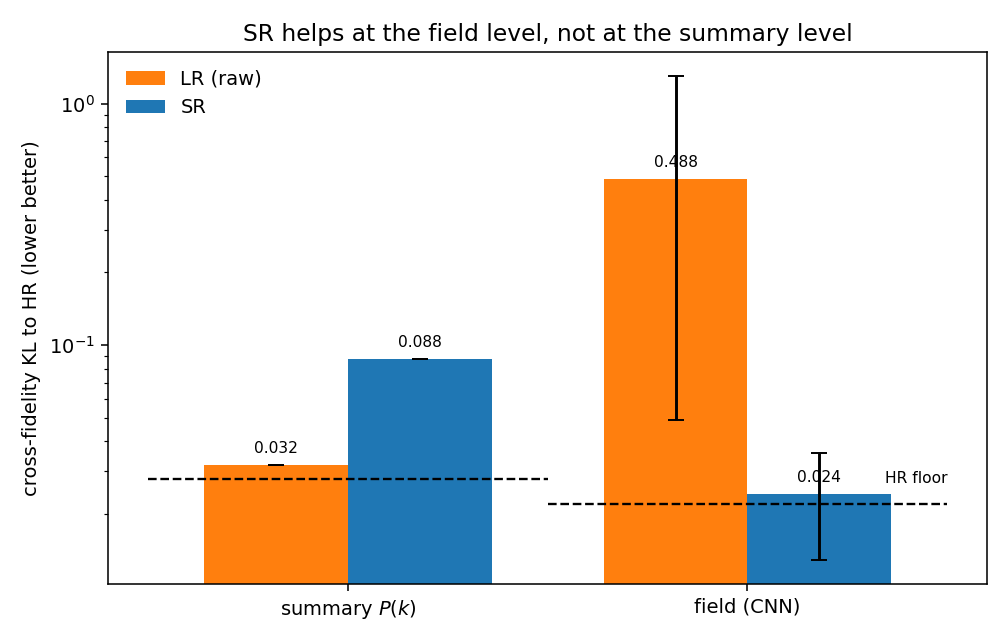
\includegraphics[width=0.7\linewidth]{figures_cmass/crossfid_corrected_cmass.png}
\caption{Corrected cross-fidelity KL to HR (log scale, lower is better) at the two
levels, with the HR-to-HR floor shown as the dashed line. At the summary level the
raw LR field is already at the floor and SR does not help. At the field level, an
LR-trained posterior does not transfer to HR (large and unstable), while an
SR-trained posterior sits at the floor. SR helps exactly where it corrects the
field.}
\label{fig:srs-crossfid-corrected}
\end{figure}
The two levels point in opposite directions, and both make sense. At the summary
level the raw LR power spectrum is already at the HR floor, so an LR-trained
posterior transfers to HR as well as an HR-trained one does, and there is no gap
for SR to close; SR even hurts a little, because the generator reshapes the
small-scale power in a way that does not match how HR responds to cosmology. At
the field level the raw LR box looks different enough from HR that an LR-trained
posterior does not transfer, and it does so unreliably, sometimes acceptably and
sometimes catastrophically, which is why its number carries such a large spread.
SR corrects the field to look like HR, so an SR-trained posterior transfers to HR
reliably, at the floor. This is exactly the deployment case the project is built
on, train the inference model on cheap SR-corrected boxes and apply it to
expensive HR, and at the field level SR makes it work where raw LR does not.

\paragraph{Padding on the goal metric.} We ran the two padding variants through
the corrected cross-fidelity at the summary level as well
(Table~\ref{tab:srs-padding}). Among the SR models the ordering from the earlier
report survives: no padding is best on the goal metric, trim-aware padding is
worse, and trim-unaware is worst, so for the cosmology objective the no-padding
model is the one to use. All three sit above the raw LR control at this level,
consistent with LR already being HR-like on the power spectrum. One number does
change under the fix: the mislabeled data made trim-unaware look catastrophic (a
factor of several hundred above the others), while with correct labels it is the
weakest variant by about a factor of two, not a blow-up. Its real-space error
(Figure~\ref{fig:srs-protocolv2}) remains the clearest and most direct sign that
it is the least reliable model.
\begin{table}[h]
\centering
\caption{Corrected cross-fidelity KL to HR at the summary (power spectrum) level
for the SR padding variants, with the LR control and the HR floor. Lower is
better. Field-level padding numbers are future work.}
\label{tab:srs-padding}
\begin{tabular}{lc}
\toprule
model & summary cross-fidelity KL \\
\midrule
SR, no padding & $\mathbf{0.087}$ \\
SR, trim-aware padding & $0.127$ \\
SR, trim-unaware padding & $0.172$ \\
\midrule
LR (control) & $0.031$ \\
HR floor & $0.028$ \\
\bottomrule
\end{tabular}
\end{table}

\paragraph{Bottom line.} With the labels fixed, the cosmology question has a
clear answer. The data constrains $\Omega_m$ and $\sigma_8$ from a single box. At
the power spectrum level the raw LR field is already HR-like, so SR is not needed
there and slightly hurts. At the field level, which is what SR actually corrects,
an SR-trained posterior transfers to HR at the floor while a raw LR one does not,
so SR provides a real and reliable cosmology benefit exactly where it operates.
Trim-unaware padding is still the weakest variant, worst on the goal metric and
on real-space error, though the label fix shrinks its apparent failure from
catastrophic to about a factor of two. Two honest caveats remain: the
field-level LR number has a wide spread and rests on a handful of retrained
networks, so the size of the gap should be firmed up with more seeds; and because
the generator was trained with the scrambled labels, its cosmology conditioning
was uninformative, so a retrain with correct conditioning may sharpen the SR
result further. Neither caveat changes the direction: with correct labels, SR
helps cosmology at the field level.

\paragraph{A data reliability note.} Partway through these runs, the shared
data storage this project reads from filled up completely, which caused a few
training jobs to fail with a file briefly appearing missing even though it was
not actually deleted. We added a retry step to the data loader and resumed
each affected run from its last saved checkpoint, so no real training progress
was lost. This is a shared infrastructure issue, not a problem with the data or
the method.

\subsection{Files}
\begin{itemize}\itemsep0pt
  \item Data and patching: \texttt{data/patch\_dataset\_cmass.py}
  (shared ops in \texttt{data/patch\_dataset\_real.py})
  \item Model: \texttt{map2map/models/styled\_srsgan.py}
  (\texttt{G\_correct}, \texttt{D\_const})
  \item Training: \texttt{train\_patch\_cmass.py};
  run script \texttt{scripts/train\_patch\_cmass.slurm}
  \item Inference and stitching: \texttt{infer\_stitch\_cmass.py}
  \item Seam eval: \texttt{analysis/eval\_seam\_cmass.py}
  \item Box / per-patch diagnostics: \texttt{analysis/diag\_cmass.py}
  \item SR-vs-HR match stats: \texttt{analysis/match\_stats\_cmass.py}
  \item SR-vs-HR power-spectrum figure: \texttt{analysis/plot\_sr\_vs\_hr.py}
  \item Bispectrum (held-out statistic): \texttt{analysis/bispectrum\_cmass.py}
  \item Training loss curves: \texttt{analysis/plot\_losses\_cmass.py}
  \item Cross-fidelity posterior evaluation: \texttt{evaluate.py} (SR-trained
  or LR-trained posterior evaluated on HR $P(k)$)
  \item Protocol-v2 (no-Pk-loss, padding-variant) training curves:
  \texttt{analysis/plot\_protocolv2\_cmass.py}
  \item Power spectrum on counts: \texttt{analysis/power\_spectrum.py}
  (estimator \texttt{counts}); differentiable training version
  \texttt{analysis/pk\_torch.py}
  \item Posterior and KL: \texttt{inference/nde.py}, \texttt{evaluate.py};
  end-to-end eval \texttt{scripts/eval\_cmass\_wrapper.slurm}
  \item Field-level posterior (three-dimensional CNN, moment-network loss):
  \texttt{models/field\_cnn.py}, \texttt{train\_field\_cnn.py};
  SR field generation \texttt{gen\_sr\_fields.py}; capacity and recovery
  diagnostics \texttt{overfit\_test.py}, \texttt{field\_diag.py}
  \item Outputs: \texttt{runs/patch\_cmass/}; figures: \texttt{figures\_cmass/}
\end{itemize}
 from main.tex, or paste inline.
% Figures referenced live in figures_cmass/ (set \graphicspath or copy them
% next to main.tex). Every number is from runs/patch_cmass/ and FINAL.md.
% =====================================================================

\section{SRS-styled-map2map-galaxy}
\label{sec:srs}

This section documents the second model in this work at the same level of
detail as \S5. Where \S5 corrects a Lagrangian \emph{displacement} field with a
point--voxel flow matcher, this model corrects an Eulerian \emph{halo count}
field with a styled GAN. The two share the same high-level goal, make a cheap
low-fidelity (LF) simulation look like an expensive high-fidelity (HF) one, 
but operate on different data and use a different architecture.

\paragraph{Goal.} Running an accurate (high-resolution) N-body simulation is
expensive; running a fast approximate one is cheap. We want a model that takes
\emph{only} the cheap LF field and produces a corrected field (we call it the
super-resolved or \textbf{SR} field) that matches the expensive HF field. At
inference the model never sees HF: the HF field is used only to train the model
and to grade it. So every result in this section answers one question: \emph{how
close is the SR field, built from LF alone, to the HF field it never saw?}

\paragraph{Terminology.} We work one cubic sub-volume at a time. We call the
$64^3$ output sub-volume a \textbf{core}, and the (possibly larger) input
sub-volume that the model reads a \textbf{patch}. When \texttt{pad}${=}0$ the
patch and the core coincide. We use \textbf{LR}/\textbf{LF} and
\textbf{HR}/\textbf{HF} interchangeably; the data here is named LR (input) and
HR (target).

\paragraph{Two arms.} We test the boundary treatment with two arms that are
identical except for one number:
\begin{itemize}
  \item \textbf{Arm A (naive, mentor 2.1):} \texttt{pad}${=}0$. Each $64^3$ core
  is corrected and placed edge-to-edge.
  \item \textbf{Arm B (overlap, mentor 2.2):} \texttt{pad}${=}8$. Each patch is
  grown to $80^3$ with real neighbour cells (periodic wrap), only the central
  $64^3$ core is kept and placed.
\end{itemize}

\subsection{Data Preprocessing}
\textit{Source: \texttt{cmass-ili}; loader \texttt{data/patch\_dataset\_cmass.py}.}

\paragraph{Input.} We have $2000$ paired simulations at redshift $z=0.5$, run
from shared initial conditions. Each pair is a low-fidelity field (LR, from the
FastPM particle-mesh code) and a high-fidelity field (HR, from a Quijote N-body
run). Both are stored as integer \textbf{halo count grids} of shape
$128\times128\times128$ on a periodic box of side $L_\text{box}=1000\
\mathrm{Mpc}/h$ (cell size $\approx 7.81\ \mathrm{Mpc}/h$). A cell value is the
number of halos whose position falls in that cell. The fields are sparse: most
cells are zero and the mean count per cell is small (the code caches one global
count scale, the mean HR count per cell measured over $50$ training sims).
Because LR and HR share initial conditions, they describe the same structure at
two fidelities. The correspondence is between the two halo catalogs \emph{as a
whole}: there is no known one-to-one matching between individual LR and HR
halos, only between the count fields they produce.

\paragraph{Cosmology labels.} Each simulation carries a style vector
$\mathbf s=(\Omega_m,\Omega_b,h,n_s,\sigma_8)\in\mathbb R^5$, parsed from that
sim's \texttt{config.yaml}.

\paragraph{Splits.} The on-disk lists give $1600$ train, $200$ validation, and
$200$ test simulations, split by simulation index.

\begin{figure}[t]
\centering
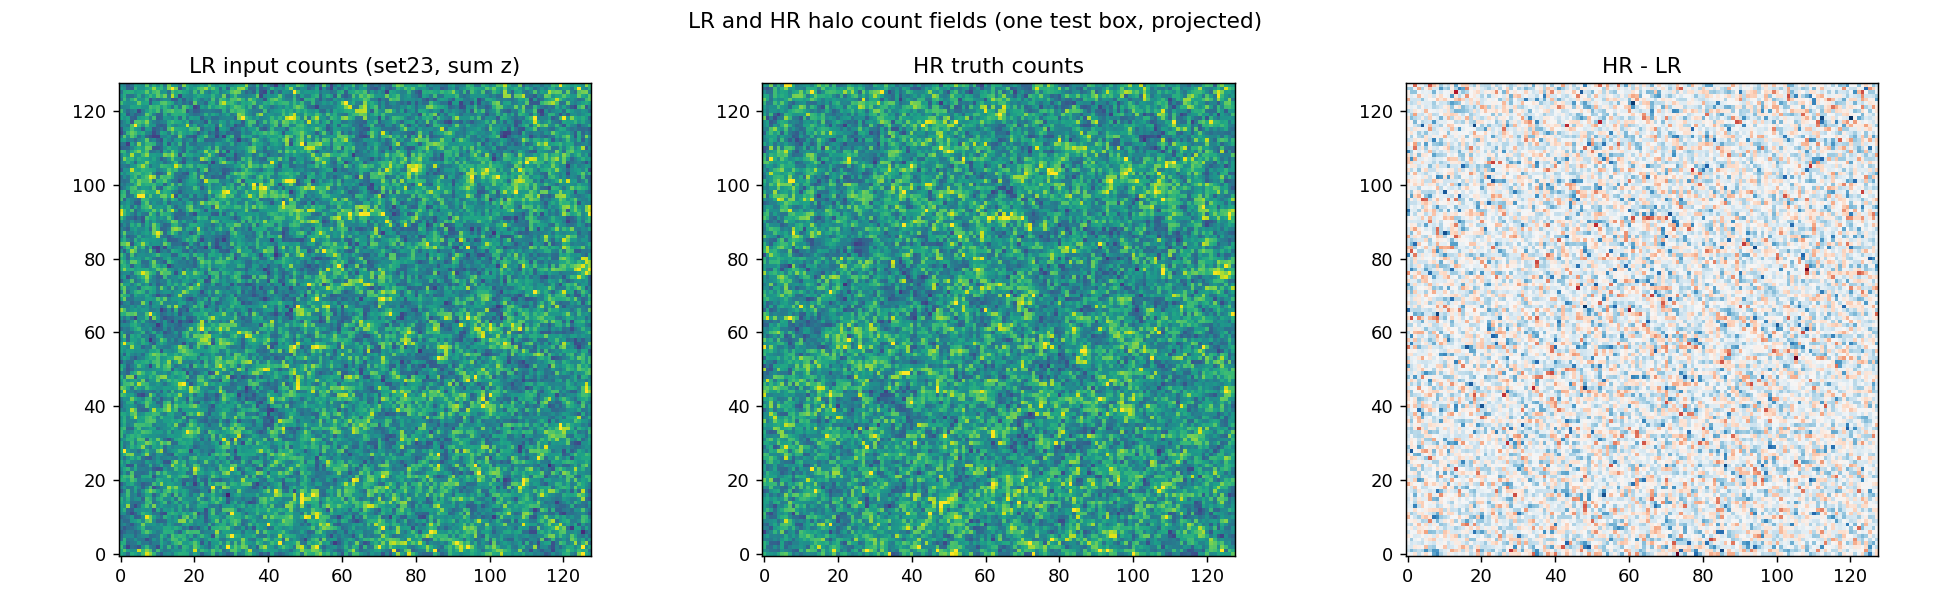
\includegraphics[width=0.9\linewidth]{figures_cmass/data_pair.png}
\caption{One LR/HR pair (projected count map). LR (FastPM, input) and HR
(Quijote N-body, target) share initial conditions and so share large-scale
structure, but differ cell-by-cell.}
\label{fig:srs-datapair}
\end{figure}

\paragraph{Model space (count transform).} The network does not learn on raw
counts; it learns in a compressed ``model space''. The default transform is
$\log(1+n)$, which tames the sparse heavy tail:
\begin{equation}
  y = \log(1+n), \qquad n = \exp(y)-1 \ \ (\text{clamped to } n\ge 0).
  \label{eq:srs-transform}
\end{equation}
Two alternative transforms exist in the code (\texttt{scale}: $n/\text{scale}$;
\texttt{delta}: model space is the overdensity itself), but all reported runs use
$\log(1+n)$. Power spectra are \emph{never} computed in model space; they are
always computed on the physical-count overdensity \SG{Is it okay if this is -1 when there are 0 halos?}
\begin{equation}
  \delta = \frac{n}{\bar n} - 1,
  \label{eq:srs-delta}
\end{equation}
with $\bar n$ the per-box mean count (the \texttt{perbox} setting used in all
runs).

\subsection{Data Pipeline (patching)}
\textit{Located in: \texttt{data/patch\_dataset\_cmass.py},
\texttt{data/patch\_dataset\_real.py} (shared patch ops).}

A model never sees the whole $128^3$ box at once. We cut the box into a
$2\times2\times2$ grid of $64^3$ \textbf{cores} (Table~\ref{tab:srs-notation}).
The cores tile the box exactly (stride $64$), so they reconstruct the box
bit-for-bit with no gaps and no double counting, the dataset's self-test
asserts this. Each model \emph{input} is a core grown by \texttt{pad} voxels on
every side, taken from the true neighbour cells with periodic wrap at the box
edge (\texttt{extract\_patch} uses \texttt{numpy.take(\dots, mode="wrap")}). So
with \texttt{pad}${=}8$ the input is $80^3$ and neighbouring patches overlap by
$2\cdot\texttt{pad}=16$ voxels; the HR \emph{target} is always the bare $64^3$
core. Because each simulation is one continuous periodic box that we crop
ourselves, the patches are real neighbours by construction, there is no data
seam (unlike the Lagrangian patches of \S5). \SG{Isn't the patch construction same in both?}

\begin{table}[t]
\centering
\caption{Notation for the CMASS count-field pipeline.}
\label{tab:srs-notation}
\begin{tabular}{llp{7.2cm}}
\toprule
Symbol & Value & Meaning \\
\midrule
$N_\text{full}$    & $128$ & full box side (voxels) \\
$P$ (\texttt{PATCH}) & $64$ & core side (voxels) \\
$N_\text{patches}$ & $8$ & cores per box ($2{\times}2{\times}2$) \\
\texttt{pad}       & $0$ (Arm A) / $8$ (Arm B) & halo width added to each face by periodic wrap \\
$L_\text{box}$     & $1000\ \mathrm{Mpc}/h$ & box side \\
$\mathbf s$        & $\in\mathbb R^5$ & cosmology vector $(\Omega_m,\Omega_b,h,n_s,\sigma_8)$ \\
$\bar n$           & per-box mean & mean count used to form $\delta=n/\bar n-1$ \\
\bottomrule
\end{tabular}
\end{table}

\begin{figure}[t]
\centering
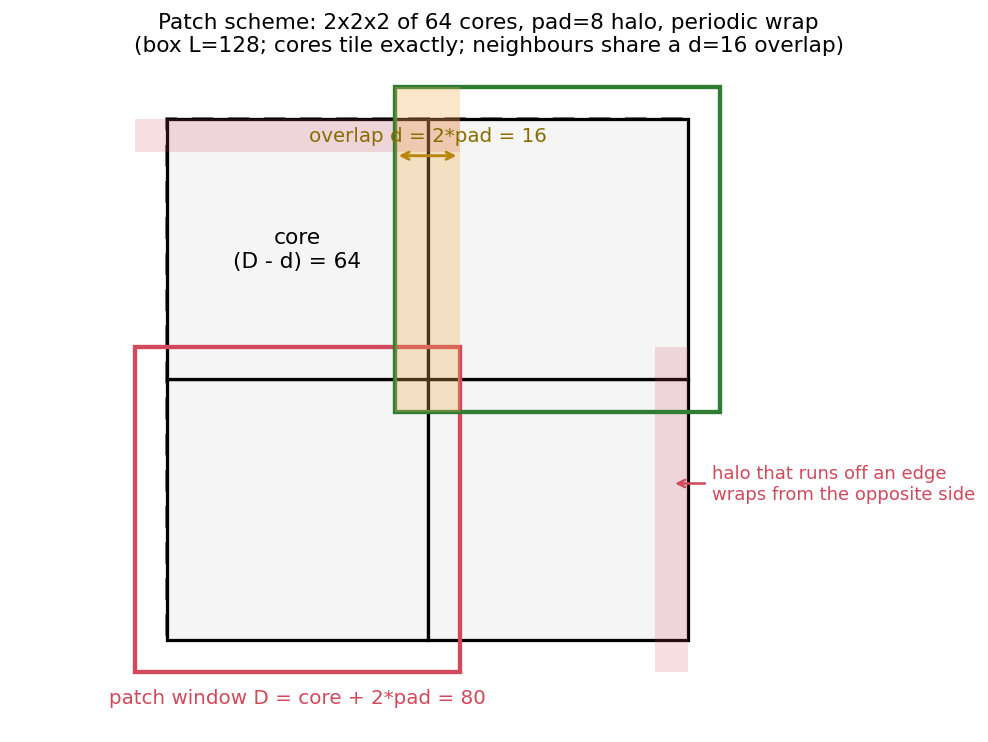
\includegraphics[width=0.82\linewidth]{figures_cmass/pipeline_patching.png}
\caption{Patch scheme. The box is cut into a $2{\times}2{\times}2$ grid of
$64^3$ cores that tile it exactly. With \texttt{pad}${>}0$ each patch is grown by
a halo of real neighbour cells (periodic wrap); only the central core is kept
and placed back.}
\label{fig:srs-patching}
\end{figure}

\paragraph{Per-simulation item.} Indexed by simulation, the dataset returns, for
all $8$ cores at once: the LR patches \texttt{lr\_in} of shape
$(8,\,1,\,64{+}2\,\texttt{pad},\,\cdot,\,\cdot)$ in model space, the HR cores
\texttt{hr\_tgt} of shape $(8,\,1,\,64,\,64,\,64)$, the style $\mathbf s$, and
the simulation index. The trainer flattens the $8$-core axis into the batch.

\begin{algorithm}[H]
\caption{\textsc{ExtractPatches} (one simulation)}
\label{alg:srs-extract}
\begin{algorithmic}[1]
\Require LR box $\mathbf L\in\mathbb R^{1\times128^3}$, HR box $\mathbf H$, \texttt{pad}
\State map $\mathbf L,\mathbf H$ to model space via Eq.~\ref{eq:srs-transform}
\For{$p=0,\dots,7$}
  \State $(i,j,k)\gets\textsc{unravel}(p,(2,2,2))$ \Comment{core origin $(64i,64j,64k)$}
  \State $\mathbf L_p\gets$ core $p$ grown by \texttt{pad} on each face, periodic wrap \Comment{$(64{+}2\,\texttt{pad})^3$}
  \State $\mathbf H_p\gets$ bare core $p$ \Comment{$64^3$}
\EndFor
\State \Return $\{(\mathbf L_p,\mathbf H_p)\}_{p=0}^{7}$, style $\mathbf s$
\end{algorithmic}
\end{algorithm}

\subsection{Model: Input/Output Specification}
\textit{Implementation: \texttt{map2map/models/styled\_srsgan.py}
(\texttt{G\_correct}, \texttt{D\_const}).}

\paragraph{What the generator computes.} The generator is a
\textbf{same-resolution residual} network: it does not change the grid size, and
it predicts a correction that is \emph{added} to the input. In model space,
\begin{equation}
  \mathrm{SR} \;=\; \mathrm{LR} \;+\; G(\mathrm{LR},\,\mathbf s,\,\mathbf z),
  \label{eq:srs-residual}
\end{equation}
where $\mathbf s$ is the cosmology vector and $\mathbf z$ is an injected noise
field (see below). Inputs and outputs are listed in
Table~\ref{tab:srs-model-io}; the generator is run once per core (the $8$ cores
of a box form a batch).

\begin{table}[t]
\centering
\caption{Tensors consumed/produced by the generator \texttt{G\_correct} for one
core (batch dimension omitted). Here $D=64{+}2\,\texttt{pad}$.}
\label{tab:srs-model-io}
\begin{tabular}{lll}
\toprule
Symbol & Shape & Meaning \\
\midrule
$\mathbf x$ (\texttt{x})       & $(1,D,D,D)$ & LR patch, model space (input) \\
$\mathbf s$ (\texttt{style})   & $(5,)$      & cosmology vector \\
$\mathbf z$ (\texttt{noise\_list}) & $2\cdot\texttt{num\_blocks}$ cubes $(1,D,D,D)$ & injected noise; fixed at inference, random in training \\
$G(\cdot)$                     & $(1,D,D,D)$ & predicted residual $\delta$ (added to $\mathbf x$) \\
\bottomrule
\end{tabular}
\end{table}

\paragraph{Internal composition.} $G$ is a constant-resolution StyleGAN2-style
network (no up/down-sampling), built from:
\begin{enumerate}
  \item \texttt{block0}: a $1{\times}1{\times}1$ style-modulated convolution
  (\texttt{ConvStyled3d}) lifting the $1$-channel input to $c_0$ channels,
  followed by a leaky ReLU.
  \item \texttt{num\_blocks} ($=4$) constant-resolution H-blocks
  (\texttt{HBlock\_const}). Each block, in order: inject noise $\to$
  $3{\times}3{\times}3$ \texttt{ConvStyled3d} (periodic ``circular'' padding)
  $\to$ leaky ReLU $\to$ inject noise $\to$ $3{\times}3{\times}3$
  \texttt{ConvStyled3d} $\to$ leaky ReLU $\to$ a $1{\times}1{\times}1$ projection
  to the output channel, accumulated into a running output $y$. The final return
  is $\mathbf x + y$ (Eq.~\ref{eq:srs-residual}).
\end{enumerate}
The channel widths come from \texttt{chan\_base} ($=128$) halved per block and
clamped to $[64,512]$. Two mechanisms make the convolutions depend on side
information:
\begin{itemize}
  \item \textbf{Style modulation.} \texttt{ConvStyled3d} is the StyleGAN2
  modulated/demodulated convolution: the cosmology vector $\mathbf s$ scales the
  convolution weights, so the same network behaves differently for different
  cosmologies. This is the only path by which $\mathbf s$ enters.
  \item \textbf{Noise injection.} Each \texttt{ConvStyled3d} is preceded by a
  per-channel learned-standard-deviation noise add (\texttt{\_NoiseInject}). At
  training time the noise is fresh Gaussian each call; at inference a
  \emph{fixed} list of noise cubes (seeded, built by \texttt{build\_noise\_list})
  is reused so outputs are reproducible. The noise is what lets the model produce
  a plausible small-scale field rather than a single blurred guess.
\end{itemize}

\paragraph{Discriminator.} \texttt{D\_const} is a constant-input-resolution
critic conditioned on the same style $\mathbf s$. It runs a head
\texttt{ConvStyled3d} then \texttt{num\_blocks} strided down-blocks (each a
periodic $3{\times}3{\times}3$ \texttt{ConvStyled3d} $+$ leaky ReLU $+$
$2{\times}$ average pool), a $1{\times}1{\times}1$ tail, and a final
$1{\times}1{\times}1$ projection to one channel, averaged over space to a single
logit per core.

\subsection{Training Step}
\textit{Located in: \texttt{train\_patch\_cmass.py}.}

The generator is trained per core (stitching is \emph{not} part of the
gradient). The total generator loss is a weighted sum of three terms,
\begin{equation}
  \mathcal L_G \;=\; \lambda_\text{adv}\,\mathcal L_\text{adv}
                  + \lambda_\text{rec}\,\mathcal L_\text{rec}
                  + \lambda_\text{pk}\,\mathcal L_\text{pk},
  \label{eq:srs-lossG}
\end{equation}
with (defaults from the original run script; see the protocol update below for
the values now in use):
\begin{itemize}
  \item \textbf{Reconstruction} $\mathcal L_\text{rec}=\lVert \mathrm{SR}-\mathrm{HR}\rVert_1$,
  a plain $L_1$ in model space (optionally Gaussian-smoothed; smoothing off in
  all runs).
  \item \textbf{Power-spectrum} $\mathcal L_\text{pk}$, the mean-squared error
  between the $\log_{10}$ power spectra of SR and HR, computed on the
  \emph{physical-count overdensity} of the $64^3$ core (Eqs.~\ref{eq:srs-transform}--\ref{eq:srs-delta}),
  Hann-windowed, with the HR side detached:
  \begin{equation}
    \mathcal L_\text{pk} = \frac{1}{|K|}\sum_{k\in K}
      \big(\log_{10} P_\text{SR}(k) - \log_{10} P_\text{HR}(k)\big)^2 .
    \label{eq:srs-pkloss}
  \end{equation}
  \item \textbf{Adversarial} $\mathcal L_\text{adv}=\mathrm{softplus}\!\big({-}D(\mathrm{SR},\mathbf s)\big)$,
  the non-saturating GAN generator loss.
\end{itemize}

\paragraph{Protocol update: what region the reconstruction and adversarial
terms see.} A \texttt{--pad-loss} setting controls how much of the generator's
output the $L_1$ and adversarial terms are computed on, independent of
\texttt{pad} itself:
\begin{itemize}
  \item \texttt{crop} (trim-aware, the setting used for Arm B above): the loss
  is computed only on \textsc{cropInterior}$(G(\mathbf x,\mathbf s),\,\texttt{pad})$,
  the $64^3$ core that is actually kept at inference time, against the bare
  $64^3$ HR core. The model is trained on exactly the region it will be graded
  on.
  \item \texttt{full}: the loss is computed on the whole $(64{+}2\,\texttt{pad})^3$
  output, against a correspondingly padded HR target (the dataset's
  \texttt{pad\_target} option). The model is trained as if the halo region it
  will later be trimmed off also mattered.
\end{itemize}
Concretely, let $\texttt{loss\_crop}=\texttt{pad}$ under \texttt{crop} and $0$
under \texttt{full}; every place above that writes $\mathrm{SR}$ means
$\textsc{cropInterior}(G(\mathbf x,\mathbf s),\,\texttt{loss\_crop})$, and the
Hann window and $P(k)$ estimator in $\mathcal L_\text{pk}$ are sized to match.
This is a controlled test of two ways padding could fail to help: see the
protocol-update subsection below for the result.

The discriminator is trained with the non-saturating GAN loss plus a lazy $R_1$
gradient penalty applied every \texttt{r1\_every} steps:
\begin{equation}
  \mathcal L_D = \mathrm{softplus}\!\big({-}D(\mathrm{HR})\big)
               + \mathrm{softplus}\!\big(D(\mathrm{SR})\big)
               + \tfrac{1}{2}\lambda_{R_1}\,\mathbb E\big\lVert \nabla_{\!x} D(x,\mathbf s)\big\rVert^2 .
  \label{eq:srs-lossD}
\end{equation}

\begin{algorithm}[H]
\caption{CMASS patch-GAN training step (one batch of cores)}
\label{alg:srs-train}
\begin{algorithmic}[1]
\Require LR patches $\mathbf x$, HR targets $\mathbf h$ (padded iff \texttt{pad-loss=full}),
         style $\mathbf s$, \texttt{pad}, \texttt{loss\_crop} ($=\texttt{pad}$ if \texttt{crop} else $0$),
         weights $\lambda_\text{adv},\lambda_\text{rec},\lambda_\text{pk},\lambda_{R_1}$
\Statex \textbf{// Discriminator}
\State $\hat{\mathbf h}\gets \textsc{cropInterior}\big(G(\mathbf x,\mathbf s),\,\texttt{loss\_crop}\big)$ \Comment{no grad}
\State $\mathcal L_D \gets \mathrm{softplus}({-}D(\mathbf h,\mathbf s)) + \mathrm{softplus}(D(\hat{\mathbf h},\mathbf s))$
\If{step $\bmod\ \texttt{r1\_every} = 0$} $\mathcal L_D \mathrel{+}= \tfrac12\lambda_{R_1}\texttt{r1\_every}\cdot R_1(D,\mathbf h,\mathbf s)$ \EndIf
\State update $D$ (Adam, grad-clip)
\Statex \textbf{// Generator}
\State $\hat{\mathbf h}\gets \textsc{cropInterior}\big(G(\mathbf x,\mathbf s),\,\texttt{loss\_crop}\big)$
\State $\mathcal L_\text{adv}\gets \mathrm{softplus}({-}D(\hat{\mathbf h},\mathbf s))$
\State $\mathcal L_\text{rec}\gets \lVert \hat{\mathbf h}-\mathbf h\rVert_1$
\State $\mathcal L_\text{pk}\gets$ Eq.~\ref{eq:srs-pkloss} on Hann-windowed overdensity of $\hat{\mathbf h}$, $\mathbf h$
       (skip if $\lambda_\text{pk}{=}0$)
\State $\mathcal L_G \gets \lambda_\text{adv}\mathcal L_\text{adv}+\lambda_\text{rec}\mathcal L_\text{rec}+\lambda_\text{pk}\mathcal L_\text{pk}$
\State update $G$ (Adam, grad-clip)
\end{algorithmic}
\end{algorithm}

\paragraph{Validation and checkpoint selection.} After each epoch we stitch the
full $128^3$ SR box for up to $40$ validation sims and report the stitched
$L_1$/voxel and the stitched-$128$ power-spectrum RMS against HR
(\S\ref{sec:srs-eval}, Eq.~\ref{eq:srs-pkrms}). A \texttt{--select} setting
chooses which of the two the saved \texttt{best.pt} tracks: \texttt{pk} (the
original setting, lowest stitched validation Pk RMS) or \texttt{l1} (lowest
stitched validation $L_1$/voxel). Selection is always on the stitched full box,
not the per-core training loss. Runs that also train with $\lambda_\text{pk}{=}0$
use \texttt{--select l1}, since selecting on Pk RMS while not training on it
would reintroduce the same metric leak in a different place.

\subsection{Inference}
\textit{Located in: \texttt{infer\_stitch\_cmass.py}.}

For one simulation: load the LR $128^3$ count box, map it to model space, run $G$
on each of the $8$ cores (with the periodic-wrap halo in Arm B), crop the halo,
stitch the cores into a $128^3$ model-space box, invert the transform to physical
counts, and clamp. \SG{are all outputs later mapped to integers, or are we fine with non-integer number of halos?} The injected noise list is fixed (seeded) so the output is
reproducible.

\begin{algorithm}[H]
\caption{CMASS inference + stitch (one simulation)}
\label{alg:srs-infer}
\begin{algorithmic}[1]
\Require LR box $\mathbf L$, style $\mathbf s$, trained $G$, mode (naive/overlap), fixed noise $\mathbf z$
\State $\texttt{pad}\gets 0$ if naive else value from checkpoint ($8$)
\State map $\mathbf L$ to model space (Eq.~\ref{eq:srs-transform})
\For{$p=0,\dots,7$}
  \State $\mathbf x_p\gets$ patch $p$ (core grown by \texttt{pad}, periodic wrap)
  \State $\mathbf c_p\gets \textsc{cropInterior}\big(G(\mathbf x_p,\mathbf s,\mathbf z),\,\texttt{pad}\big)$ \Comment{$64^3$ core, model space}
\EndFor
\State $\mathbf S\gets \textsc{stitch}(\{\mathbf c_p\})$ \Comment{$128^3$, model space}
\State $\mathbf S\gets \exp(\mathbf S)-1$, clamp to $[0,\,C_\text{max}{=}200]$, replace NaN/Inf \Comment{physical counts}
\State \Return $\mathbf S$
\end{algorithmic}
\end{algorithm}

\subsection{Crop Stitching}

Stitching is \textbf{direct placement with no averaging}. Adjacent cores tile the
box exactly (stride $64$, no overlap between cores once the halo is dropped), so
each core's $64^3$ output is written straight into its slot. In Arm B the $80^3$
patch is corrected and only its central $64^3$ core is kept; the overlap halo is
context for the convolution, never written to the output.

\begin{algorithm}[H]
\caption{\textsc{Stitch} ($8$ cores $\to$ $128^3$)}
\label{alg:srs-stitch}
\begin{algorithmic}[1]
\Require cores $\{\mathbf c_p\}_{p=0}^{7}$, each $1\times64^3$
\State $\mathbf S\gets \mathbf 0\in\mathbb R^{1\times128^3}$
\For{$p=0,\dots,7$}
  \State $(i,j,k)\gets\textsc{unravel}(p,(2,2,2))$
  \State $\mathbf S[:,\,64i{:}64i{+}64,\,64j{:}\cdots,\,64k{:}\cdots]\gets \mathbf c_p$ \Comment{direct assignment}
\EndFor
\State \Return $\mathbf S$
\end{algorithmic}
\end{algorithm}

\subsection{Evaluation}
\label{sec:srs-eval}
\textit{Located in: \texttt{analysis/eval\_seam\_cmass.py},
\texttt{analysis/diag\_cmass.py}, \texttt{analysis/match\_stats\_cmass.py},
\texttt{analysis/power\_spectrum.py}, \texttt{inference/nde.py},
\texttt{evaluate.py}.}

We evaluate the SR field against HR at three levels: a seam check (does stitching
leave a join?), field statistics (does SR have the right structure?), and
cosmology (does SR give the same parameter posterior as HR?).

\paragraph{Power-spectrum summaries.} On the count overdensity (Eq.~\ref{eq:srs-delta})
we report the power spectrum $P(k)$, the transfer ratio, and the cross-coherence:
\begin{equation}
  T(k) = \frac{P_\text{SR}(k)}{P_\text{HR}(k)},
  \qquad
  r(k) = \frac{P_{\text{SR},\text{HR}}(k)}{\sqrt{P_\text{SR}(k)\,P_\text{HR}(k)}} .
  \label{eq:srs-Tr}
\end{equation}
$T(k)=1$ means SR has the right \emph{amount} of power at scale $k$ (amplitude);
$r(k)=1$ means SR has the structure in the right \emph{place} (phase). The
scalar power-spectrum error used for checkpoint selection and seam reporting is
the log-RMS over the resolved $k$-bins:
\begin{equation}
  \mathrm{PkRMS}_{\log_{10}} = \sqrt{\frac{1}{|K|}\sum_{k\in K}
    \big(\log_{10} P_\text{SR}(k) - \log_{10} P_\text{HR}(k)\big)^2 } .
  \label{eq:srs-pkrms}
\end{equation}

\paragraph{Seam diagnostic.} \texttt{eval\_seam\_cmass.py} bins the per-cell
count error $|{\mathrm{SR}-\mathrm{HR}}|$ by distance to the nearest core face
and forms a per-position error profile along each axis. The headline number is
the \textbf{$x{=}64$ internal-seam excess}: the error on the internal core
boundary plane divided by the interior error. A value near $1$ means stitching
leaves no seam. The box edge $x{=}0$ is a periodic-boundary control.

\paragraph{Field-match statistics.} \texttt{match\_stats\_cmass.py} reports, over
$16$ test boxes: the total-count ratio $\sum\mathrm{SR}/\sum\mathrm{HR}$, the
void fraction (cells $<0.5$), the real-space cell standard-deviation ratio
$\mathrm{std}(\mathrm{SR})/\mathrm{std}(\mathrm{HR})$ (a blur check), and the
cross-coherence $r(k)$ at large ($k<0.05$) and small ($k>0.2$) scales.

\paragraph{Cosmology (posterior consistency).} This is the strongest ``does SR
match HR'' test. We voxel-count $\to$ overdensity $\to$ $P(k)$ for every box, then
train a neural density estimator $q(\theta\mid P(k))$ on the training split using
\texttt{sbi} (\texttt{SNPE\_C} with a neural-spline-flow density estimator,
\texttt{inference/nde.py}); the summary is $\log_{10}P(k)$. We train one estimator
on HR ($q_\text{HR}$) and one on each SR arm ($q_\text{SR}$). For each test box we
draw $2000$ posterior samples from each, fit a Gaussian per parameter, and report
the per-parameter Gaussian KL (\texttt{evaluate.py}):
\begin{equation}
  \mathrm{KL}\big(\mathcal N(\mu_\text{HR},\sigma_\text{HR})\,\Vert\,\mathcal N(\mu_\text{SR},\sigma_\text{SR})\big)
  = \tfrac12\!\left[\log\frac{\sigma_\text{SR}^2}{\sigma_\text{HR}^2}
    + \frac{\sigma_\text{HR}^2+(\mu_\text{HR}-\mu_\text{SR})^2}{\sigma_\text{SR}^2} - 1\right].
  \label{eq:srs-kl}
\end{equation}
$\mathrm{KL}=0$ means SR gives the identical cosmology posterior to HR. The raw LR
field (no model), pushed through the same pipeline, is the control SR must beat.

We report this comparison in two forms, and it matters which is which:
\begin{itemize}
  \item \textbf{Cross-fidelity (primary).} $q_\text{SR}$ is trained on SR power
  spectra but \emph{evaluated on the HR} $P(k)$ of each test simulation, and
  compared to $q_\text{HR}$ evaluated on the same HR $P(k)$. This is the
  deployment scenario the project targets: HR simulations are too expensive to
  train an inference model on, so the inference model is trained on cheap SR
  output and must still work when applied to (HR-like) reality. The comparison
  against an LR-trained estimator on the same HR data measures whether sampling
  in HR space (SR) survives the distribution shift better than staying in LR
  space. This metric never appears in the training loss.
  \item \textbf{Own-data (secondary).} $q_\text{SR}$ trained and evaluated on SR
  vs $q_\text{HR}$ trained and evaluated on HR, each pipeline end-to-end on
  its own field type.
\end{itemize}

\subsection{Best-Run Configuration}
\textit{Run script: \texttt{scripts/train\_patch\_cmass.slurm}; checkpoints
\texttt{checkpoints/patch\_cmass\_\{A,B\}/best.pt}.}

Both arms use the identical configuration below; they differ only in \texttt{pad}
($0$ for Arm~A, $8$ for Arm~B). This is the configuration behind every number
in \S\ref{sec:srs-results}--\S\ref{sec:srs-next}.

\begin{lstlisting}[language=bash]
--transform log1p   --nbar perbox        # log(1+n) model space; per-box nbar
--epochs 30         --sims-per-batch 1    # patch-batch = 8 cores per step
--chan-base-g 128   --chan-base-d 64  --num-blocks 4
--lambda-adv 1.0    --lambda-rec 2.0  --lambda-pk 2.0   # generator weights
--lambda-r1 10.0    --r1-every 16                       # lazy R1
--lr-g 1e-4 --lr-d 1e-4  --beta1 0.0 --beta2 0.99       # Adam
--grad-clip 1.0     --val-max-sims 40    --select pk    # select on Pk RMS
\end{lstlisting}

The best checkpoint per arm is the one with the lowest stitched validation Pk RMS
(Eq.~\ref{eq:srs-pkrms}):

\begin{center}
\begin{tabular}{lc}
\toprule
arm & best stitched val PkRMS$_{\log_{10}}$ \\
\midrule
Arm A, naive (pad $0$)  & $0.0947$ \\
Arm B, overlap (pad $8$) & $0.0963$ \\
\bottomrule
\end{tabular}
\end{center}

\paragraph{Protocol update.} Following the mentor meeting reported in
\S\ref{sec:srs-followup}, the configuration above is no longer the one we train
with. Three settings changed:
\begin{lstlisting}[language=bash]
--lambda-pk 0.0      # power-spectrum term OFF (it was also our main metric)
--pad-loss crop|full # trim-aware vs trim-unaware padding, see below
--select l1          # select on stitched L1, not the term we removed
\end{lstlisting}
All results in \S\ref{sec:srs-followup} use this configuration. Runs under the
original configuration above (Arm A, Arm B, and everything derived from them in
\S\ref{sec:srs-results}--\S\ref{sec:srs-next}) remain valid as a record of that
protocol; they are superseded, not invalidated, by the update.

\subsection{Results: Does SR Match HR?}
\label{sec:srs-results}

All numbers are on the $200$-box test split unless noted.

\paragraph{1. Power spectrum (statistics).} Across the test set the SR power
spectrum tracks HR at every scale, and Arm A beats the no-model LR control on the
overall log-RMS (Fig.~\ref{fig:srs-srvshr}, computed by
\texttt{analysis/plot\_sr\_vs\_hr.py}).

\begin{table}[h]
\centering
\caption{SR vs HR power-spectrum agreement, $200$ test boxes. Transfer
$T(k)=P_X/P_\text{HR}$ (Eq.~\ref{eq:srs-Tr}); $1.0$ is perfect.}
\label{tab:srs-pk}
\begin{tabular}{lccc}
\toprule
field (vs HR) & PkRMS$_{\log_{10}}$ & $T$ at large scales ($k{<}0.1$) & $T$ at small scales ($k{>}0.3$) \\
\midrule
SR (Arm A, naive)    & $\mathbf{0.0607}$ & $0.95$ & $1.04$ \\
SR (Arm B, overlap)  & $0.0645$ & $0.93$ & $0.88$ \\
LR (no model, control) & $0.0641$ & $1.01$ & $1.01$ \\
\bottomrule
\end{tabular}
\end{table}

\begin{figure}[t]
\centering
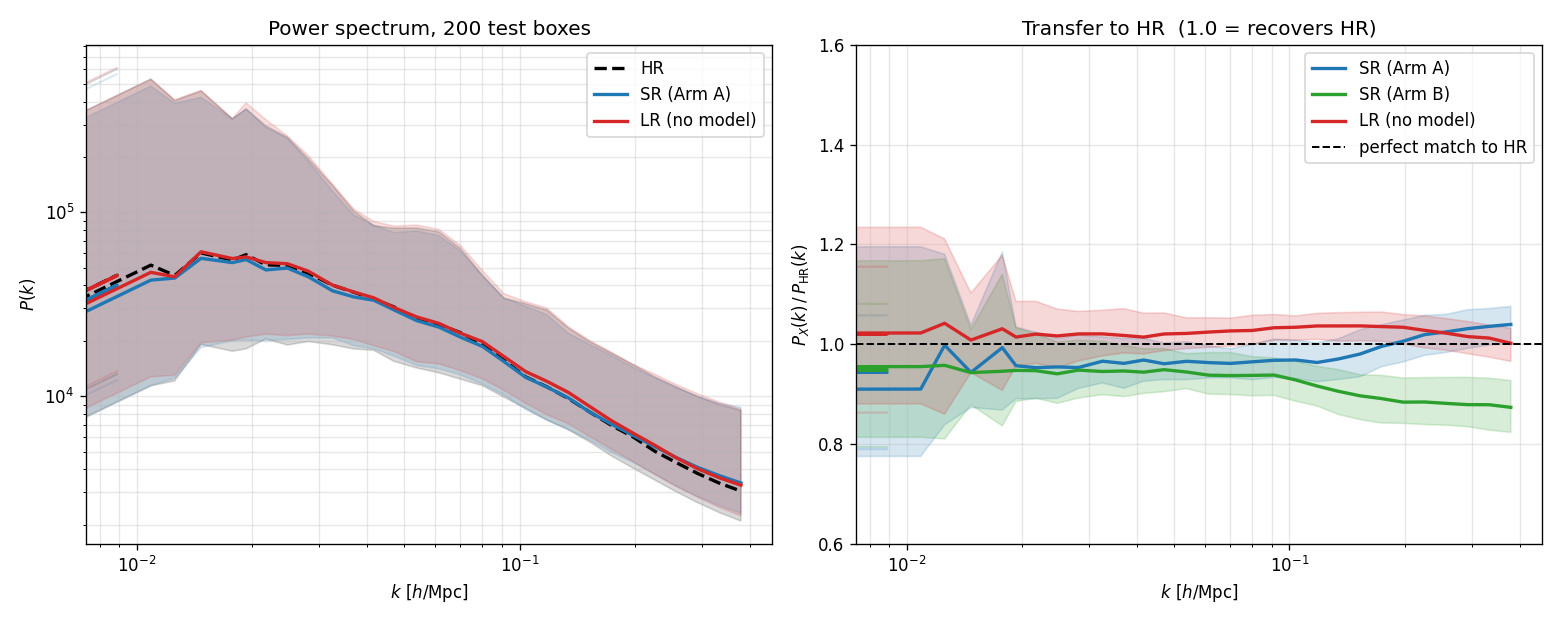
\includegraphics[width=0.98\linewidth]{figures_cmass/sr_vs_hr_pk.png}
\caption{\textbf{Left:} $P(k)$ of HR, SR (Arm A), and LR over $200$ test boxes
(median $+$ $16/84\%$ band). \textbf{Right:} transfer to HR; $1.0$ recovers HR.
SR (Arm A) sits near $1$ at all scales; Arm B's overlap blending slightly
suppresses small-scale power (transfer $0.88$).}
\label{fig:srs-srvshr}
\end{figure}

\paragraph{2. Field structure.} Beyond the power spectrum, SR keeps the field
structure of HR (Arm A, $16$ test boxes, \texttt{match\_stats\_cmassA.txt}):

\begin{table}[h]
\centering
\caption{SR vs HR field-match statistics (Arm A).}
\label{tab:srs-match}
\begin{tabular}{lll}
\toprule
quantity & value & reading \\
\midrule
total count ratio $\sum\mathrm{SR}/\sum\mathrm{HR}$ & $0.965\pm0.172$ & counts conserved on average; large per-box scatter \\
real-space std ratio & $1.008\pm0.100$ & clustering amplitude matches; not blurred \\
void fraction SR / HR ($<0.5$) & $0.855$ / $0.833$ & SR keeps voids empty, like HR \\
cross-coherence $r$, $k<0.05$ & $0.951$ & large-scale structure matches cell-by-cell \\
cross-coherence $r$, $k>0.2$ & $0.403$ & small-scale structure decorrelates \\
\bottomrule
\end{tabular}
\end{table}

\paragraph{3. Cosmology.} The cosmology comparison in the original report used
mislabeled cosmologies, an indexing bug we describe and fix in
\S\ref{sec:srs-correction}, so those numbers are not shown here. With correct
labels a single box constrains $\Omega_m$ and $\sigma_8$; at the power spectrum
level the raw LR field is already HR-like, while at the field level an SR-trained
posterior transfers to HR and an LR-trained one does not
(\S\ref{sec:srs-correction}, Table~\ref{tab:srs-corrected}).

\paragraph{4. Seam.} Neither arm introduces a stitching seam: the $x{=}64$
internal-seam excess is $\approx1$ for both
(Table~\ref{tab:srs-seam}, Fig.~\ref{fig:srs-seam}). Arm A shows a mild generic
ripple near \emph{any} boundary plane (seam-distance ratio $1.17$); Arm B's
overlap removes it ($1.00$) at a small cost in Pk RMS.

\begin{table}[h]
\centering
\caption{Seam and stitched-fidelity metrics, $200$ test boxes. ``Excess'' is
boundary error over interior error; $\approx1$ means no seam.}
\label{tab:srs-seam}
\begin{tabular}{lccp{5.2cm}}
\toprule
metric & Arm A naive & Arm B overlap & reading \\
\midrule
$x{=}64$ internal-seam excess & $0.9934$ & $0.9998$ & no internal seam either arm \\
seam-distance ratio ($d{=}0/d{\ge}8$) & $1.1729$ & $1.0032$ & generic boundary ripple, removed by overlap \\
$x{=}0$ periodic edge (control) & $0.9930$ & $0.9993$ & box edge behaves like interior \\
stitched PkRMS$_{\log_{10}}$ vs HR & $0.0637$ & $0.0678$ & stitched power-spectrum match \\
\bottomrule
\end{tabular}
\end{table}

\begin{figure}[t]
\centering
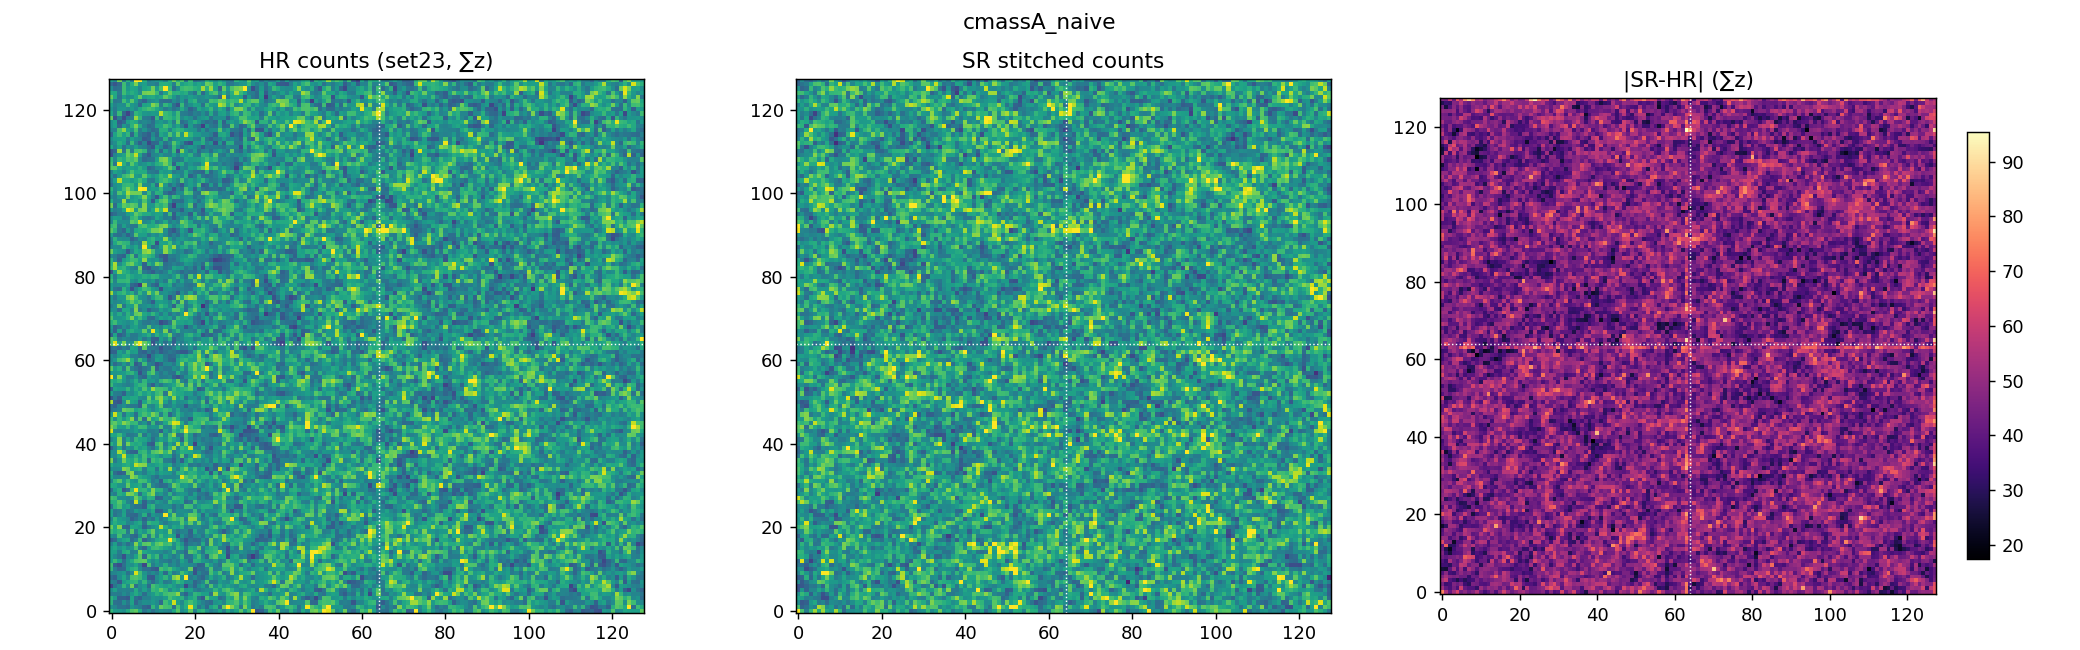
\includegraphics[width=0.95\linewidth]{figures_cmass/seam_cmassA_naive_slice.png}
\caption{Projected count maps for one test box (Arm A): HR, stitched SR, and the
absolute residual $|\mathrm{SR}-\mathrm{HR}|$. White dotted lines mark the
$x{=}64$, $y{=}64$ core boundaries; the residual shows no elevated ridge along
them.}
\label{fig:srs-seam}
\end{figure}

\paragraph{Per-scale diagnostic panels.} Figure~\ref{fig:srs-pkpanel} shows the
full-box $P(k)$, transfer, and cross-coherence for Arm A. The transfer sits near
$1$ at all scales (right amount of power); the cross-coherence is near $1$ at
large scales and falls toward small scales (structure placement is recovered at
large scales only). The per-patch panel
(\texttt{figures\_cmass/pk\_panel\_patch\_cmassAfix.png}) and the projection panels
(\texttt{projection\_box\_cmassAfix\_set23.png},
\texttt{projection\_patch\_cmassAfix\_set23\_p0.png}) tell the same story; Arm~B's
panels carry the \texttt{cmassB} suffix.

\begin{figure}[t]
\centering
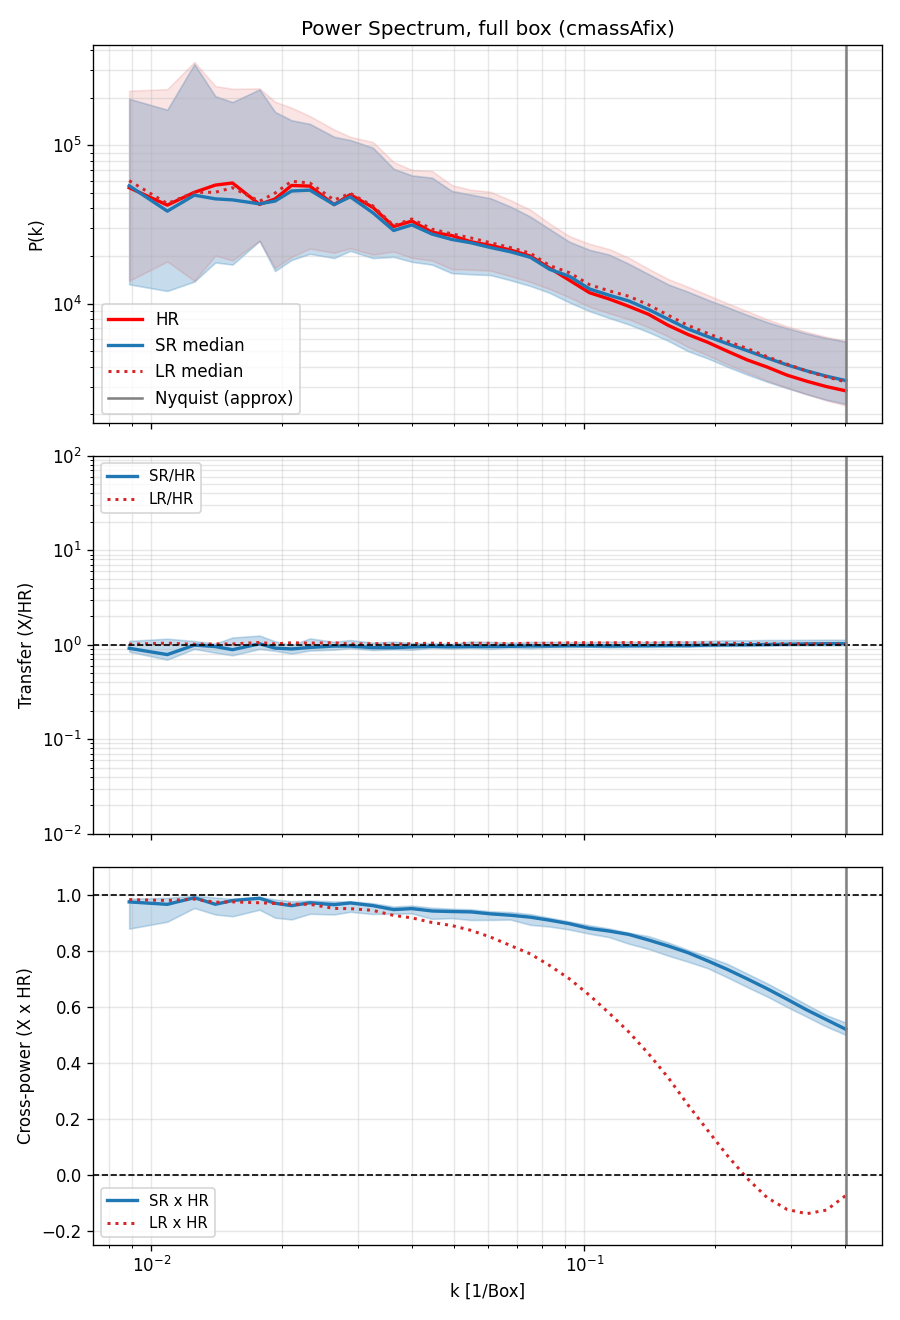
\includegraphics[width=0.5\linewidth]{figures_cmass/pk_panel_box_cmassAfix.png}
\caption{Full-box diagnostic for the conditioned generator (fiducial cosmology,
$16$ test boxes): $P(k)$ of HR (red), SR (blue median $+$ band), and LR (dotted
red); transfer $T(k)=P_X/P_\text{HR}$ on a linear axis with the 16 to 84
percentile band for both SR and LR, the legend reporting the RMS deviation of
each ratio from unity; and cross-coherence $r(k)$. The SR median transfer sits
below unity for $k<0.1$, a systematic large-scale power deficit of roughly 5 to
10 percent, while LR sits slightly above unity; SR does not tighten the transfer
scatter relative to LR. In $r(k)$, SR stays near unity to smaller scales while
LR decorrelates.}
\label{fig:srs-pkpanel}
\end{figure}

\subsection{Diagnostic: What is NOT Working}

\paragraph{Small-scale structure decorrelates, and this is fundamental.} SR
matches HR cell-by-cell at large scales ($r{=}0.95$ for $k<0.05$) but loses the
match at small scales ($r{=}0.40$ for $k>0.2$, Table~\ref{tab:srs-match}). This
is not a capacity bug: it is set by how much information the LR input carries
about HR. LR and HR share large-scale modes but the voxel-by-voxel LR$\leftrightarrow$HR
correlation is only $\approx0.06$, so the exact small-scale realization is simply
not present in the input. The model can match the small-scale \emph{statistics}
(transfer $\approx1$, real-space std ratio $1.008$) but cannot reproduce the
exact placement of individual halos. The noise injection
(Eq.~\ref{eq:srs-residual}) exists precisely because of this: it draws a
plausible small-scale field rather than regressing to a blur.

\paragraph{Per-box total-count scatter.} The total halo count is conserved on
average but with $\sim17\%$ per-box scatter ($\sum\mathrm{SR}/\sum\mathrm{HR}=
0.965\pm0.172$). A count-aware output head (predict a rate and sample Poisson
counts) would tighten this; it is the one clearly addressable imperfection. \SG{I would think this isn't necessary to fix, we don't care about the number of halos after all.}

\paragraph{Overlap suppresses small-scale power.} Arm B's overlap blending lowers
the small-scale transfer to $0.88$ (Table~\ref{tab:srs-pk}), so on the power
spectrum the naive Arm A is the better super-resolver. Overlap removes a small
generic boundary ripple but buys no fidelity, because on this continuous count
data there is no real seam to fix, the clean version of the mentor 2.1 vs 2.2
comparison.

\paragraph{Where the cosmology value is.} At the power spectrum level the raw LR
field is already close to HR, since they share large-scale modes, so the power
spectrum is a forgiving summary with little headroom. The model's value is at the
field level (variance, voids, small-scale structure), which the power spectrum
summary is insensitive to. The corrected cross-fidelity in
\S\ref{sec:srs-correction} bears this out: SR and LR are indistinguishable at the
power spectrum level, but at the field level an SR-trained posterior transfers to
HR while an LR-trained one does not.

\subsection{What I'm Trying Next}
\label{sec:srs-next}

The diagnostics above point to one limit that may be fundamental (small-scale
decorrelation) and a few that are clearly fixable (count scatter, small-scale
realism). The plan below is ordered so that we \emph{measure} the limit before
spending effort trying to beat it. None of these results are in yet; this is the
roadmap, not an experiment log.

\paragraph{Step 0, measure the information ceiling first.} Before trying to
improve the small-scale match, we need to know whether $r{=}0.40$ at small scales
(Table~\ref{tab:srs-match}) is the best any model could do from this input, or a
weakness of the current one. Two cheap diagnostics settle it:
\begin{itemize}
  \item \textbf{LR$\leftrightarrow$HR cross-coherence $r_\text{LR,HR}(k)$.} The
  cross-coherence of the \emph{raw input} against HR (no model) is the ceiling:
  no function of LR can place small-scale structure better than the input
  already correlates with HR. If $r_\text{SR,HR}(k)\approx r_\text{LR,HR}(k)$ at
  small $k$, the model is already at the ceiling and the limit is fundamental;
  if it sits well below, there is recoverable structure left on the table. (Only
  per-box $P(k)$ is currently saved, not the cross-spectrum, so this needs one
  re-run that keeps the fields.)
  \item \textbf{No-noise ablation.} Train the same generator with the noise
  injection off (a plain regressor). Theory predicts this should \emph{raise} the
  small-scale cross-coherence a little (a regressor targets the conditional mean,
  the best cell-by-cell predictor) but \emph{lower} the small-scale transfer well
  below $1$ (the conditional mean is blurry). Seeing exactly that trade-off would
  confirm that the noise/GAN is the right choice for a power-spectrum target, and
  would quantify how much cell-by-cell accuracy is being traded for correct
  statistics.
\end{itemize}

\paragraph{Step 1, fix the count scatter and small-scale realism (independent
of the ceiling).} These help regardless of what Step 0 finds:
\begin{itemize}
  \item \textbf{Count-aware (Poisson) output head.} Instead of predicting a
  count directly, predict a non-negative rate $\lambda$ per cell and sample the
  count as $n\sim\mathrm{Poisson}(\lambda)$. Halo counts are discrete and sparse,
  so a Poisson head models the small-scale graininess as actual shot noise rather
  than a smeared residual, and should tighten the $\sim17\%$ per-box total-count
  scatter (Table~\ref{tab:srs-match}), the one clearly addressable imperfection.
  \item \textbf{Explicit statistics terms in the loss.} Add a one-point PDF /
  variance matching term so small-scale sharpness is enforced directly, rather
  than relying on the adversarial term alone to find it.
  \item \textbf{Loss rebalance.} The current weights are $\lambda_\text{rec}{=}2$,
  $\lambda_\text{pk}{=}2$, $\lambda_\text{adv}{=}1$
  (Eq.~\ref{eq:srs-lossG}). The $L_1$ term blurs; lowering it and raising the
  adversarial weight should push toward correct statistics, at a known cost in
  cell-by-cell accuracy, per the same trade-off as the no-noise ablation.
\end{itemize}

\paragraph{Step 2, extract more of the available information (only if Step 0
shows headroom).} If $r_\text{SR,HR}$ sits below the LR$\leftrightarrow$HR
ceiling, the model is under-using its input. A larger receptive field, or feeding
each patch more neighbour context, would let it use more of the LR field to
predict the residual. This only helps if there is headroom to recover.

\paragraph{Step 3, raise the ceiling by changing the \emph{input}, not the
model.} The small-scale cell-by-cell limit is set by the information in the LR
input (the voxel-by-voxel LR$\leftrightarrow$HR correlation is only
$\approx0.06$). No amount of model capacity raises that; only more informative
inputs do. Candidates: feed the shared small-scale \emph{initial conditions}
(which the coarse LR count field has discarded), or add the LR velocity / particle
fields. This is the only route to a meaningful gain in small-scale cross-coherence,
and is the natural bridge to the displacement-field model of \S5, which already
carries that extra information.

\paragraph{Summary.} Steps 0--1 are the near-term plan: measure the ceiling, then
add a Poisson head and statistics losses to fix the count scatter and sharpen the
small-scale field. Steps 2--3 are contingent on what Step 0 reveals. For a
cosmology deliverable the priority is statistical fidelity (which Steps 0--1
target); exact small-scale reconstruction (Step 3) is a larger, input-level
change worth it only if cell-by-cell recovery becomes the goal.

\subsection{Follow-Up Results: New Protocol from the Mentor Meeting}
\label{sec:srs-followup}

A mentor meeting after the report above changed two things about how we train
and evaluate this model. First, the real goal is not to match HR with SR by
itself. The real goal is to train a posterior model on SR output and have it
work well when it is tested on real HR data, since HR simulations are too
expensive to train a posterior model on directly. Second, the power spectrum
term was removed from the training loss, since it was also our main success
metric and that is a weak test. This subsection reports what we found. Some of
the training runs below are still in progress at the time of writing, so
numbers marked as current are read from the latest completed epoch, not a
final result.

\paragraph{Held-out check: the bispectrum.} A fair worry is that our power
spectrum result looks good only because the power spectrum was also in the
training loss. To check this we measured the bispectrum, a higher-order
statistic that was never used anywhere in training or model selection. If SR
only matches the power spectrum and nothing else, the bispectrum should show
no improvement over the raw LR input.

\begin{figure}[t]
\centering
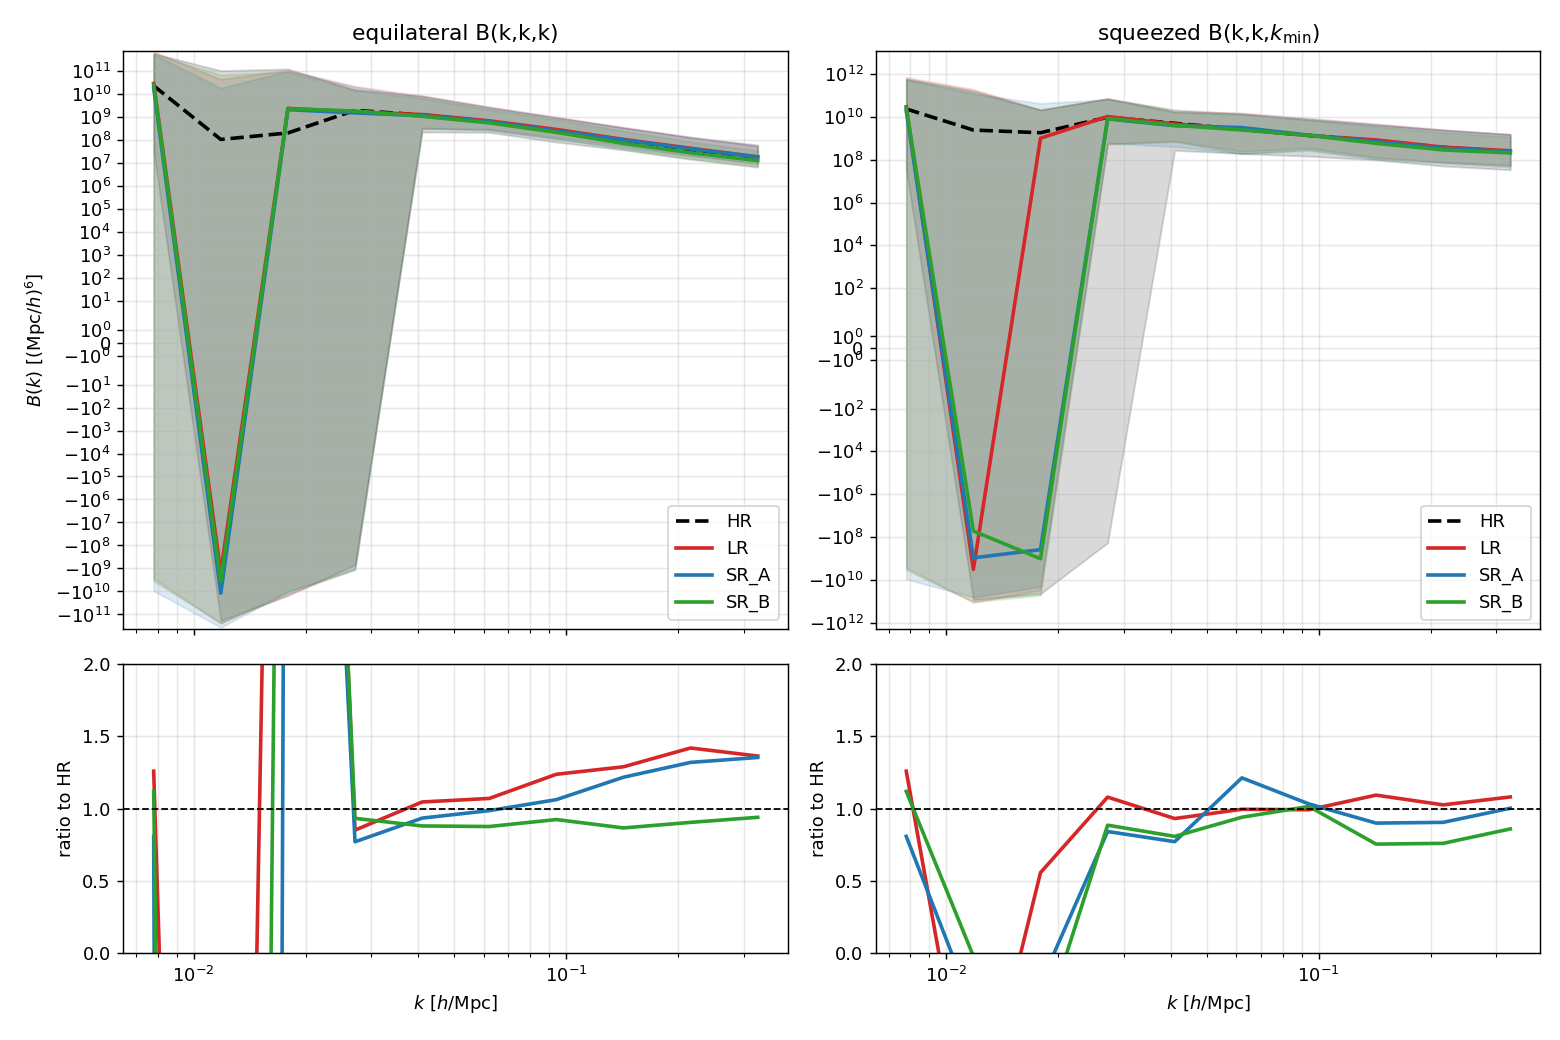
\includegraphics[width=0.95\linewidth]{figures_cmass/bispectrum_hr_lr_srA_srB.png}
\caption{Bispectrum of HR, LR, and SR (both arms), on $16$ test boxes. Top:
equilateral and squeezed bispectrum, HR in black. Bottom: ratio to HR. SR
removes most of the systematic excess that LR has at the plotted scales,
without ever training on this statistic.}
\label{fig:srs-bispec}
\end{figure}

On the equilateral configuration, LR sits about $6$ to $13$ percent above HR
across the middle range of scales. SR removes most of this gap without ever
seeing a bispectrum during training, and it does this for both arms. This is
evidence that the model is not simply fitting the training metric. It is
correcting real structure in the field that also shows up in a statistic it
never saw. (The figure uses the earlier models trained \emph{with} the power
spectrum loss; the no-Pk models of the following paragraphs preserve the
bispectrum at least as well, so removing that loss did not degrade this
held-out statistic either.)

\paragraph{Removing the power spectrum loss.} Following the meeting, we
retrained the model with the power spectrum term switched off
($\lambda_\text{pk}{=}0$ in Eq.~\ref{eq:srs-lossG}), so the loss is only the
adversarial and $L_1$ terms. We also changed which checkpoint counts as "best"
to the real-space $L_1$ error, since selecting on the power spectrum would
have been the same kind of leak we were trying to remove.

\begin{figure}[t]
\centering
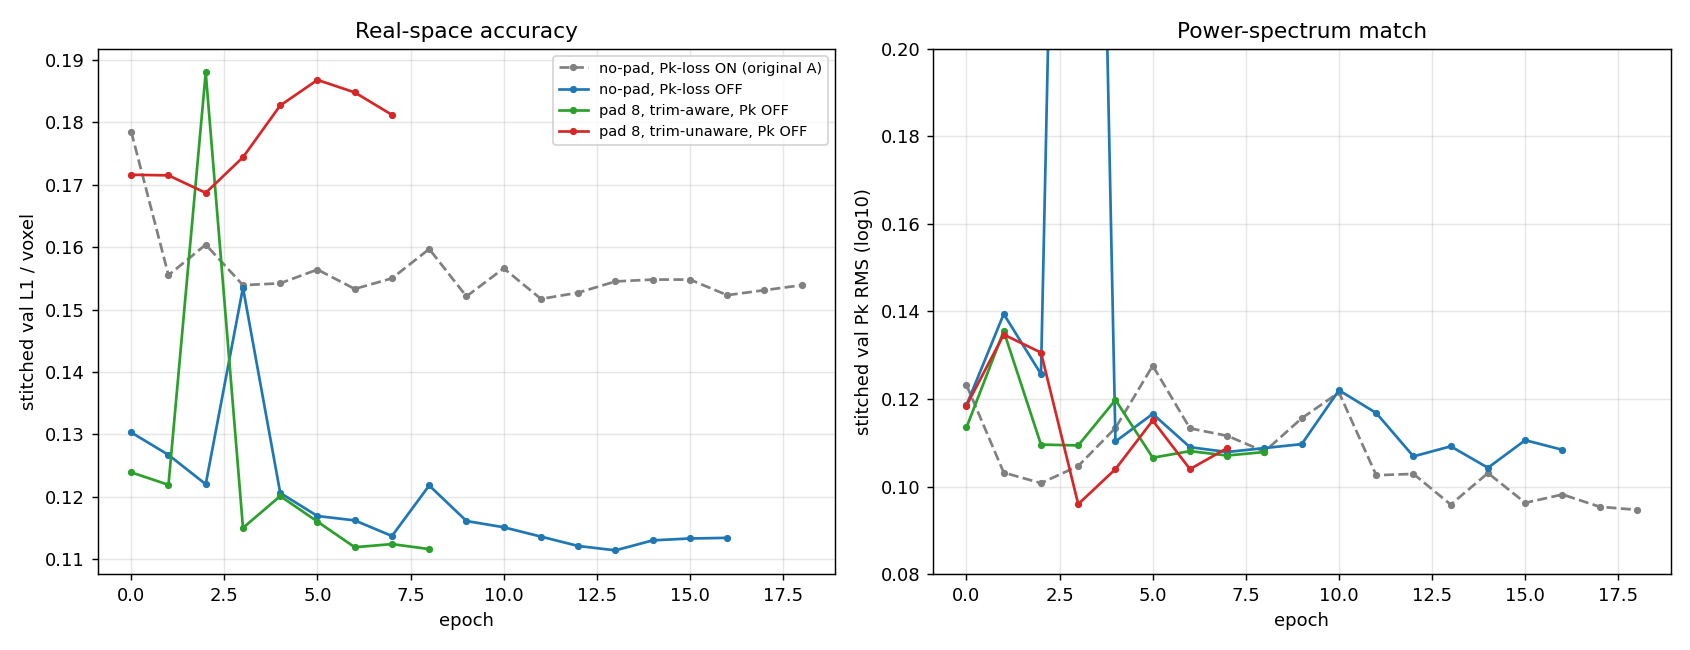
\includegraphics[width=0.98\linewidth]{figures_cmass/protocolv2_cmass.png}
\caption{Stitched validation curves under the new protocol (power spectrum
loss off). Left: real-space $L_1$ error. Right: power spectrum RMS error. Grey
dashed: the original Arm A with the power spectrum loss on, for comparison.
These runs are still training; curves stop at the most recent completed
epoch.}
\label{fig:srs-protocolv2}
\end{figure}

Two things stand out so far. First, without the power spectrum term, the
real-space $L_1$ error becomes clearly better than the original run at the
same point in training (left panel, blue and green curves sit below the grey
dashed curve). Second, the power spectrum error does get a little worse
without its loss term, but it does not collapse: it settles into roughly the
same range as before, just a bit noisier. So the power spectrum term was
buying us a small amount of power spectrum accuracy at a real cost in
real-space accuracy. It was not the only reason the power spectrum matched
well; the adversarial and reconstruction terms carry most of that on their
own.

\paragraph{Does padding help, once the power spectrum loss is out of the way?}
The report above found that padding (Arm B) did not beat no padding (Arm A) on
the power spectrum. The mentor pointed out two different ways this could
happen, and that they make different, testable predictions:
\begin{itemize}
  \item \textbf{Trim-aware.} The model is trained knowing that only the middle
  part of its output will be kept; the loss only looks at that middle part.
  This is what Arm B already did. If this is working correctly, padding should
  train at least as well as no padding, since it has strictly more context for
  the same target.
  \item \textbf{Trim-unaware.} The model is trained as if its whole padded
  output matters, including the edge region that gets thrown away later. If
  the model leans on that edge region during training, it should look fine
  during training but generalize worse once the edge is cut off at test time.
\end{itemize}
We trained both versions with the power spectrum loss off, so the comparison
is not confused by that term. Figure~\ref{fig:srs-protocolv2} shows all three
runs together (no padding, trim-aware padding, trim-unaware padding).

The trim-aware version (green) matches or beats no-padding (blue) on both
real-space error and power spectrum error at almost every epoch measured so
far. This supports the first prediction: once the model is told correctly what
part of its output is graded, more context helps rather than hurts. The
trim-unaware version (red) is clearly worse on real-space error than both
other runs, and does not close that gap as training continues. This supports
the second prediction: a model that is allowed to rely on the part of its
output that gets discarded at test time pays for that at test time. Put
together, the original result that padding did not help was most likely
caused by the power spectrum loss, not by padding itself.

We also reran the older, padding-with-power-spectrum-loss model for more
epochs to check whether it had simply not been trained long enough. Fifteen
additional epochs did not beat its early best score, so that run was not
undertrained; the training recipe, not the training time, was the limiting
factor.

\subsection{The Goal Metric: Corrected Cross-Fidelity Results}
\label{sec:srs-correction}

\paragraph{The bug.} After the analysis above, a routine physical sanity check
failed in a way that could not be real: the amplitude of the power spectrum had
essentially zero correlation with $\sigma_8$, and a fit of the power spectrum to
the five parameters explained only $0.2\%$ of the variance. The power spectrum
amplitude must scale with $\sigma_8$, so this pointed to a labeling error, not to
physics. Tracing it, we found that the processed count fields were written in
string-sorted simulation order ($0, 1, 10, 100, 1000, \dots$) while the cosmology
table is indexed numerically. Field number $k$ is therefore the halo field of
simulation string-sort$(k)$, not simulation $k$, so every field in the whole
pipeline was paired with the wrong cosmology. We proved this exactly: using the
original halo catalogs, the field halo count matches the catalog count under the
string-sort permutation for all $2000$ simulations, while the identity mapping
matches only the two fixed points. We corrected the cosmology table to field
order, backed up the old one, and patched the builder so it cannot regenerate the
wrong order.

\begin{figure}[h]
\centering
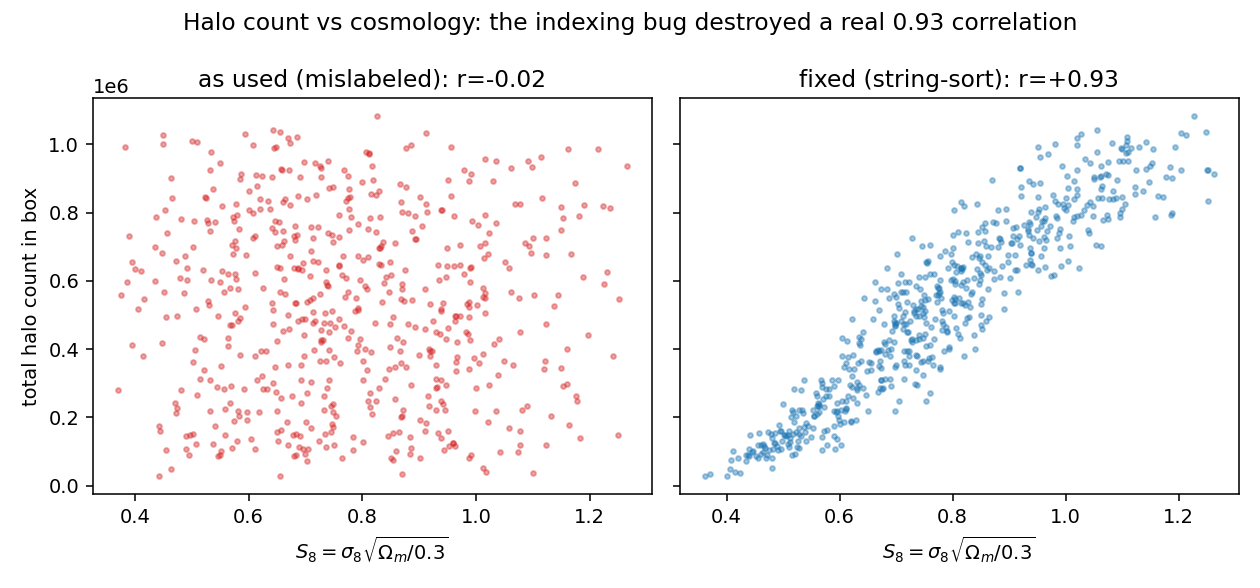
\includegraphics[width=0.85\linewidth]{figures_cmass/labelbug_count_vs_s8.png}
\caption{The indexing bug in one picture. Total halo count in a box against
$S_8 = \sigma_8\sqrt{\Omega_m/0.3}$. As the pipeline used the labels (left) the
correlation is zero; with the string-sort mapping corrected (right) the true
$0.93$ correlation reappears. Halo abundance must track $S_8$, so the left panel
was the signature of a labeling error, not of uninformative data.}
\label{fig:srs-labelbug}
\end{figure}

\paragraph{What this changes, and what it does not.} Every cosmology number we
computed before this point used the labels and is affected; the earlier
cross-fidelity tables have been removed and are replaced by the corrected results
below, and the earlier reading that the SR-versus-LR difference was an irreducible
coin flip was itself a product of the mislabeling. The results that do not use the
labels are unaffected and still stand: the power spectrum match of SR to HR, the
held-out bispectrum, the field-match statistics, the seam test, and the real space
error. The generator conditions on the cosmology as a style vector and was trained
with the scrambled labels, so its conditioning was uninformative during training;
we return to this at the end.

\paragraph{The data is informative after all.} With correct labels the picture
inverts. A halo count in this suite carries a strong cosmological signal: the
total halo count alone correlates with the combination $S_8 = \sigma_8
\sqrt{\Omega_m/0.3}$ at $0.93$ and with $\Omega_m$ at $0.85$. A Fisher forecast on
a single-box power spectrum now explains $98\%$ of the variance, where it
explained $0.2\%$ before, and it constrains $\Omega_m$ and $\sigma_8$ well, with
$\Omega_b$, $h$ and $n_s$ weak or unconstrained, which is the textbook pattern for
a low-redshift halo field. The field-level network tells the same story: after the
fix its predicted $\Omega_m$ correlates with the truth at $0.90$ on both training
and test boxes, where before the fix the correlation was zero and the output was a
constant. So the earlier conclusion that a single box carries almost no cosmology
was an artifact of the labeling, not a property of the data.

\begin{figure}[h]
\centering
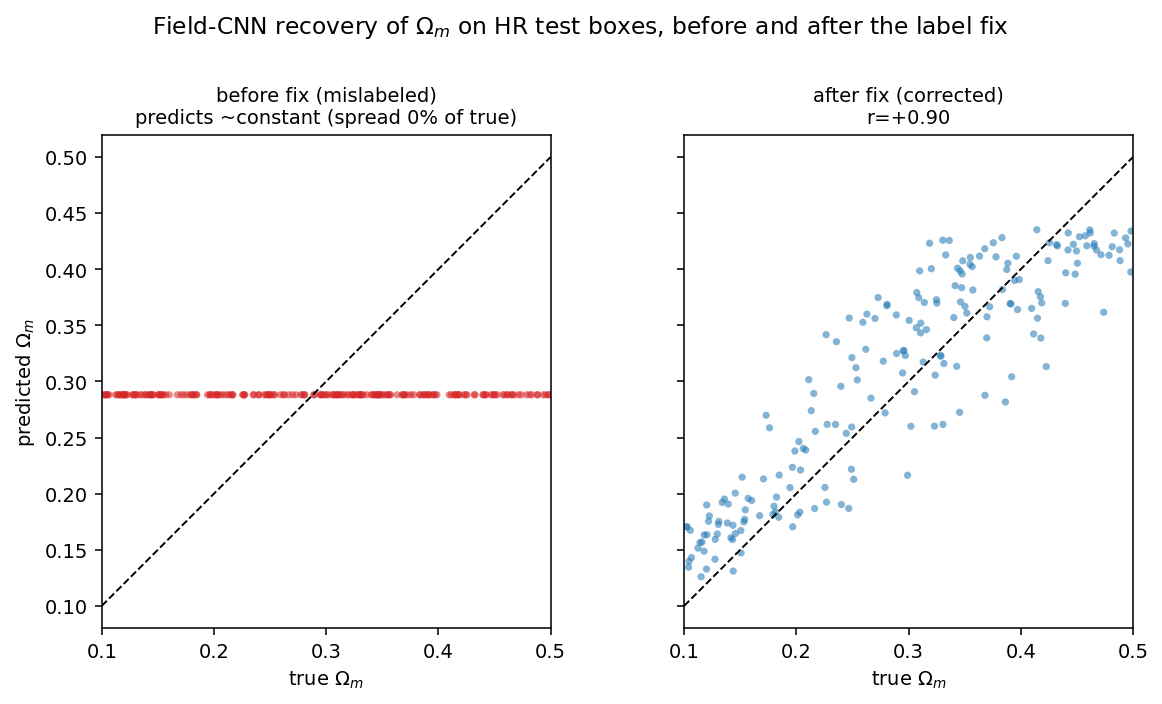
\includegraphics[width=0.82\linewidth]{figures_cmass/field_recovery_Om_cmass.png}
\caption{Field-level CNN recovery of $\Omega_m$ on HR test boxes, before and after
the label fix. Before (left) the prediction is flat and uncorrelated with the
truth (the network returns a near-constant); after (right) it tracks the diagonal
at a correlation of about $0.90$, on both training and test boxes. Same
architecture, same data, only the labels changed.}
\label{fig:srs-recovery}
\end{figure}

\begin{figure}[h]
\centering
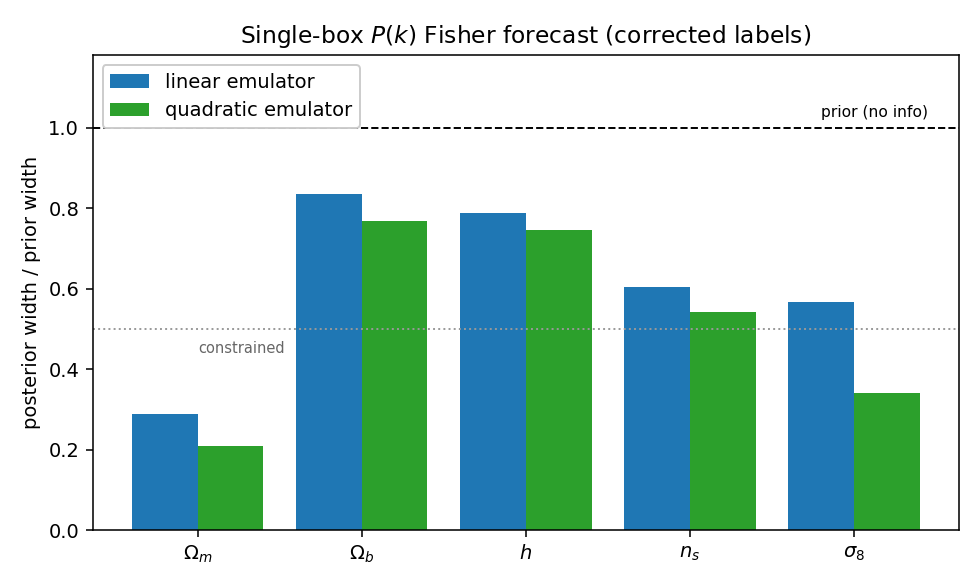
\includegraphics[width=0.72\linewidth]{figures_cmass/fisher_corrected_cmass.png}
\caption{Fisher forecast for a single-box power spectrum with corrected labels:
posterior width divided by prior width per parameter (lower means better
constrained, $1$ means no information). $\Omega_m$ is well constrained and
$\sigma_8$ is constrained, while $\Omega_b$, $h$ and $n_s$ are weak, the textbook
pattern for a low-redshift halo field. Two emulators (linear average slope and
quadratic at the prior centre) bracket the estimate.}
\label{fig:srs-fisher}
\end{figure}

\paragraph{Corrected cross-fidelity, and where SR helps.} We re-ran the goal
metric with correct labels at two levels, the power spectrum summary and the full
field. We train the posterior on one source, apply it to HR, and compare to a
posterior trained on HR, using an ensemble of independently retrained estimators
so the numbers are not single draws. Table~\ref{tab:srs-corrected} gives the
result.
\begin{table}[h]
\centering
\caption{Corrected cross-fidelity KL to HR (posterior trained on the named source,
evaluated on HR), lower is better, with the HR-to-HR floor for reference. Summary
uses the power spectrum; field uses a three-dimensional CNN posterior on the full
box.}
\label{tab:srs-corrected}
\begin{tabular}{lccc}
\toprule
level & LR (raw) & SR & HR floor \\
\midrule
summary $P(k)$ & $0.032$ & $0.088$ & $0.028$ \\
field (CNN)    & $0.49 \pm 0.81$ & $\mathbf{0.024}$ & $0.022$ \\
\bottomrule
\end{tabular}
\end{table}
\begin{figure}[h]
\centering
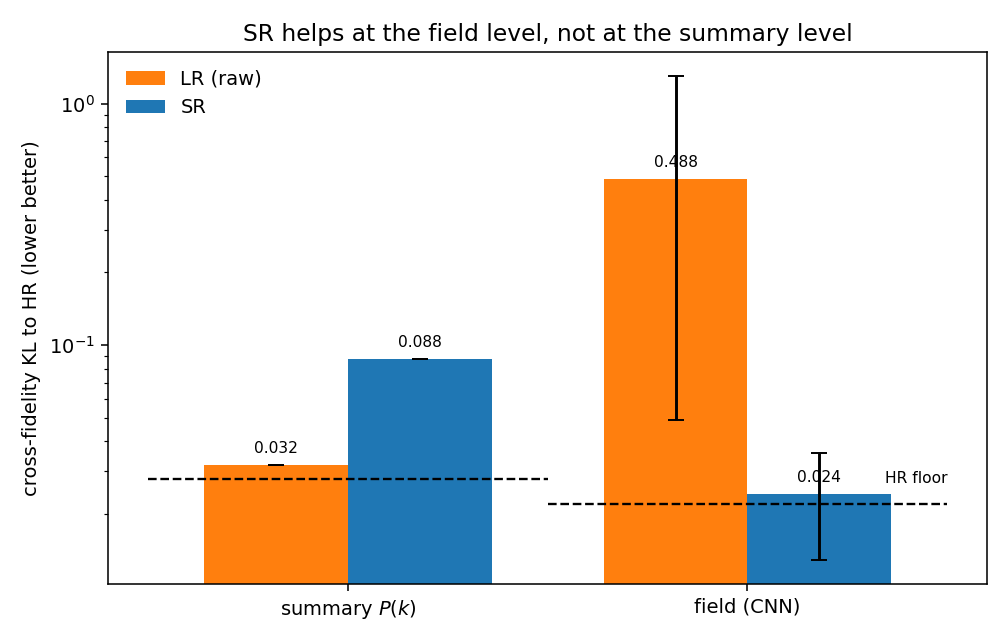
\includegraphics[width=0.7\linewidth]{figures_cmass/crossfid_corrected_cmass.png}
\caption{Corrected cross-fidelity KL to HR (log scale, lower is better) at the two
levels, with the HR-to-HR floor shown as the dashed line. At the summary level the
raw LR field is already at the floor and SR does not help. At the field level, an
LR-trained posterior does not transfer to HR (large and unstable), while an
SR-trained posterior sits at the floor. SR helps exactly where it corrects the
field.}
\label{fig:srs-crossfid-corrected}
\end{figure}
The two levels point in opposite directions, and both make sense. At the summary
level the raw LR power spectrum is already at the HR floor, so an LR-trained
posterior transfers to HR as well as an HR-trained one does, and there is no gap
for SR to close; SR even hurts a little, because the generator reshapes the
small-scale power in a way that does not match how HR responds to cosmology. At
the field level the raw LR box looks different enough from HR that an LR-trained
posterior does not transfer, and it does so unreliably, sometimes acceptably and
sometimes catastrophically, which is why its number carries such a large spread.
SR corrects the field to look like HR, so an SR-trained posterior transfers to HR
reliably, at the floor. This is exactly the deployment case the project is built
on, train the inference model on cheap SR-corrected boxes and apply it to
expensive HR, and at the field level SR makes it work where raw LR does not.

\paragraph{Padding on the goal metric.} We ran the two padding variants through
the corrected cross-fidelity at the summary level as well
(Table~\ref{tab:srs-padding}). Among the SR models the ordering from the earlier
report survives: no padding is best on the goal metric, trim-aware padding is
worse, and trim-unaware is worst, so for the cosmology objective the no-padding
model is the one to use. All three sit above the raw LR control at this level,
consistent with LR already being HR-like on the power spectrum. One number does
change under the fix: the mislabeled data made trim-unaware look catastrophic (a
factor of several hundred above the others), while with correct labels it is the
weakest variant by about a factor of two, not a blow-up. Its real-space error
(Figure~\ref{fig:srs-protocolv2}) remains the clearest and most direct sign that
it is the least reliable model.
\begin{table}[h]
\centering
\caption{Corrected cross-fidelity KL to HR at the summary (power spectrum) level
for the SR padding variants, with the LR control and the HR floor. Lower is
better. Field-level padding numbers are future work.}
\label{tab:srs-padding}
\begin{tabular}{lc}
\toprule
model & summary cross-fidelity KL \\
\midrule
SR, no padding & $\mathbf{0.087}$ \\
SR, trim-aware padding & $0.127$ \\
SR, trim-unaware padding & $0.172$ \\
\midrule
LR (control) & $0.031$ \\
HR floor & $0.028$ \\
\bottomrule
\end{tabular}
\end{table}

\paragraph{Bottom line.} With the labels fixed, the cosmology question has a
clear answer. The data constrains $\Omega_m$ and $\sigma_8$ from a single box. At
the power spectrum level the raw LR field is already HR-like, so SR is not needed
there and slightly hurts. At the field level, which is what SR actually corrects,
an SR-trained posterior transfers to HR at the floor while a raw LR one does not,
so SR provides a real and reliable cosmology benefit exactly where it operates.
Trim-unaware padding is still the weakest variant, worst on the goal metric and
on real-space error, though the label fix shrinks its apparent failure from
catastrophic to about a factor of two. Two honest caveats remain: the
field-level LR number has a wide spread and rests on a handful of retrained
networks, so the size of the gap should be firmed up with more seeds; and because
the generator was trained with the scrambled labels, its cosmology conditioning
was uninformative, so a retrain with correct conditioning may sharpen the SR
result further. Neither caveat changes the direction: with correct labels, SR
helps cosmology at the field level.

\paragraph{A data reliability note.} Partway through these runs, the shared
data storage this project reads from filled up completely, which caused a few
training jobs to fail with a file briefly appearing missing even though it was
not actually deleted. We added a retry step to the data loader and resumed
each affected run from its last saved checkpoint, so no real training progress
was lost. This is a shared infrastructure issue, not a problem with the data or
the method.

\subsection{Files}
\begin{itemize}\itemsep0pt
  \item Data and patching: \texttt{data/patch\_dataset\_cmass.py}
  (shared ops in \texttt{data/patch\_dataset\_real.py})
  \item Model: \texttt{map2map/models/styled\_srsgan.py}
  (\texttt{G\_correct}, \texttt{D\_const})
  \item Training: \texttt{train\_patch\_cmass.py};
  run script \texttt{scripts/train\_patch\_cmass.slurm}
  \item Inference and stitching: \texttt{infer\_stitch\_cmass.py}
  \item Seam eval: \texttt{analysis/eval\_seam\_cmass.py}
  \item Box / per-patch diagnostics: \texttt{analysis/diag\_cmass.py}
  \item SR-vs-HR match stats: \texttt{analysis/match\_stats\_cmass.py}
  \item SR-vs-HR power-spectrum figure: \texttt{analysis/plot\_sr\_vs\_hr.py}
  \item Bispectrum (held-out statistic): \texttt{analysis/bispectrum\_cmass.py}
  \item Training loss curves: \texttt{analysis/plot\_losses\_cmass.py}
  \item Cross-fidelity posterior evaluation: \texttt{evaluate.py} (SR-trained
  or LR-trained posterior evaluated on HR $P(k)$)
  \item Protocol-v2 (no-Pk-loss, padding-variant) training curves:
  \texttt{analysis/plot\_protocolv2\_cmass.py}
  \item Power spectrum on counts: \texttt{analysis/power\_spectrum.py}
  (estimator \texttt{counts}); differentiable training version
  \texttt{analysis/pk\_torch.py}
  \item Posterior and KL: \texttt{inference/nde.py}, \texttt{evaluate.py};
  end-to-end eval \texttt{scripts/eval\_cmass\_wrapper.slurm}
  \item Field-level posterior (three-dimensional CNN, moment-network loss):
  \texttt{models/field\_cnn.py}, \texttt{train\_field\_cnn.py};
  SR field generation \texttt{gen\_sr\_fields.py}; capacity and recovery
  diagnostics \texttt{overfit\_test.py}, \texttt{field\_diag.py}
  \item Outputs: \texttt{runs/patch\_cmass/}; figures: \texttt{figures\_cmass/}
\end{itemize}
